\documentclass[9pt,xcolor={dvipsnames},fleqn]{beamer}
%\documentclass[handout,9pt,xcolor={dvipsnames},fleqn]{beamer}
\usepackage{isse}


\usepackage{apalike}
\usepackage[utf8]{inputenc}
\usepackage{pdfpages}
%\usepackage{ngerman}
\usepackage{stmaryrd,amsmath,amssymb}
\usepackage{color}
\usepackage{enumerate}
\usepackage[makeroom]{cancel}
\usepackage{mdframed}
\usepackage{xskak}
\usepackage{fancyvrb}
\usepackage{marvosym}
\setchessboard{
showmover=false}
\usepackage[noend]{algpseudocode}   % package for algorithms
\usepackage{algorithm}
\usepackage{tikz}

\usepackage[absolute,overlay]{textpos}

\usetikzlibrary{trees,calc,shapes,arrows,matrix,shadows,decorations.markings}
\usetikzlibrary{decorations.pathreplacing}
\usetikzlibrary{calc,shapes.callouts,shapes.arrows}
\usetikzlibrary{decorations.text}

\newcommand{\CustomCite}[1]{\color{issegrey} \textbf{#1}}
\tikzset{
   hierNode/.style={main node,text width=1.1em,text centered,inner sep=1pt},
   bStyle/.style={fill=forestgreen!35},
   cStyle/.style={fill=black!35},
   dStyle/.style={fill=thermicred!25},
   optboundaries/.style={
           state,
           rectangle,
           rounded corners,
           draw=black, thick,
           minimum height=4em,
           minimum width=7em,
           inner sep=2pt,
           text centered,
           dashed
           },
  trajectory/.style={issegrey,-},
  emph/.style={isseorange},
  trajectorynode/.style={fill=issegrey},
  hystate/.style={
           state,
           rectangle,
           rounded corners,
           draw=black, very thick,
           minimum height=1em,
           minimum width=2em,
           inner sep=1pt,
           text centered,
           },
 hystatel/.style={
 		   hystate, 
 		   inner sep=3pt
 }
}


\mdfdefinestyle{theoremstyle}{
linecolor=red,linewidth=2pt,
frametitlerule=true,
frametitlebackgroundcolor=gray!20,
innertopmargin=\topskip,
}
\definecolor{LRed}{rgb}{1,.8,.8}
\definecolor{MRed}{rgb}{1,.6,.6}
\definecolor{HRed}{rgb}{1,.2,.2}

\usepackage{listings}
\lstdefinelanguage{mzn}
{
		morekeywords={var,morph,let,in,pareto,lex,par,offers,int,solve,output,not,search,satisfy,new,endif,maximize,params,instantiates,with,bool,in,type,PVS,PVSType,minimize,float,constraint,soft,sum,forall,exists,array,of,include,predicate,then,commit,post,set,function,if,else,repeat,next,ann,break},
	sensitive=false,
	morecomment=[l]{\%},
	morecomment=[s]{/*}{*/},
	morestring=[b]",
}


\definecolor{lightlightgray}{gray}{0.95}
\definecolor{forestgreen}{HTML}{009B55}
\definecolor{thermicred}{rgb}{0.82, 0.1, 0.26}
\lstset
{
	basicstyle=\ttfamily\small,
	commentstyle=\ttfamily\color{thermicred},
	stringstyle=\ttfamily\color{isseorange},
	keywordstyle=\ttfamily\color{blue},
	tabsize=2,
	showstringspaces=false,
	flexiblecolumns=true,
	captionpos=b,	
	backgroundcolor=\color{lightlightgray},
	frame=single,
	 xleftmargin=\parindent,
}

\lstset{language=mzn}
\interfootnotelinepenalty=10000

% ====== custom commands

\newcommand{\prosumer}[1]{\ensuremath{\mathtt{#1}}}
% Soft Constraint Example
\newcommand{\constraintName}[1]{\ensuremath{\mathtt{#1}}}
% Biogas Constraints
\newcommand{\biogas}{biogas}
\newcommand{\biogasShort}{bio}
\newcommand{\gasFull}{\ensuremath{\constraintName{gasNotFull}_\mathtt{\biogasShort}}}
\newcommand{\ecoSweet}{\ensuremath{\constraintName{ecoSweet}_\mathtt{\biogasShort}}}
\newcommand{\onOff}{\ensuremath{\constraintName{onOff}_\mathtt{\biogasShort}}}
% Thermal Plant Constraints
\newcommand{\thermal}{thermal}
\newcommand{\thermalShort}{therm}
\newcommand{\ecoOpt}{\ensuremath{\constraintName{ecoOpt}_\mathtt{\thermalShort}}}
\newcommand{\inertia}{\ensuremath{\constraintName{inertia}_\mathtt{\thermalShort}}}
\newcommand{\ecoGood}{\ensuremath{\constraintName{ecoGood}_\mathtt{\thermalShort}}}
\newcommand{\hLevelThermal}[1]{$H_#1^\mathtt{\thermalShort}$}
% Electric Vehicle
\newcommand{\ev}{EV}
\newcommand{\limitBatteryUsage}{\ensuremath{\constraintName{limitBU}_\mathtt{\ev}}}
\newcommand{\prefBatteryLevel}{\ensuremath{\constraintName{prefBL}_\mathtt{\ev}}}
\newcommand{\earlyBird}{\ensuremath{\constraintName{BLmorning}_\mathtt{\ev}}}
% Organization
\newcommand{\org}{org}
\newcommand{\minMaxViolation}{\ensuremath{\constraintName{violation}_\mathtt{\org}}}
\newcommand{\hLevelOrg}[1]{$H_#1^\mathtt{\org}$}

\newcommand{\Variable}{X}
\newcommand{\LocalVariable}{\widehat{\Variable}}
\newcommand{\Domain}{D}
\newcommand{\Constraint}{C}
\newcommand{\ConstraintRelationship}{\mathcal{R}}

\newcommand{\valuation}{v}
\newcommand{\constraint}[1]{\mathrm{#1}}

\newcommand{\plantconstraint}[3]{  
\ifx#1b \constraint{best}[#3]
\else \ifx#1g \constraint{good}[#3]
\else \ifx#1a \constraint{acc}[#3]
\else \ifx#1d \constraint{diff}
\else \ifx#1l \constraint{low}[#3]
\else \ifx#1h \constraint{high}[#3]
\else \ifx#1o \constraint{org}[#3]
   \else
   \constraint{#1}_{#2}^{#3} 
   
   
\fi \fi \fi \fi \fi \fi \fi}
\usepackage{stmaryrd}

\providecommand{\smyth}[1]{\prec^{#1}}
\providecommand{\smytheq}[1]{\preceq^{#1}}

\providecommand{\checkfull}{\color{ForestGreen} \checkmark}
\providecommand{\checkhalf}{\color{BurntOrange} (\checkmark)}
\providecommand{\checknot}{\color{BrickRed} $x$}
% booktabs, tables 
\usepackage{booktabs}
\usepackage{tabularx}
\usepackage{longtable}
\usepackage{dcolumn}
\newcolumntype{R}{>{\raggedleft\arraybackslash}X}
\newcolumntype{d}[1]{D{.}{.}{#1} }
\newcolumntype{L}[1]{>{\raggedright\let\newline\\\arraybackslash\hspace{0pt}}m{#1}}


\newcommand{\RN}[1]{%
  \textup{\uppercase\expandafter{\romannumeral#1}}%
}

\newcommand{\code}[1]{\normalfont\texttt{\spaceskip=3pt\frenchspacing\def\{{\char123}\def\}{\char125}\def\^{\char94}\def\_{\char95}#1}}
\newcommand{\varit}[1]{{\frenchspacing\ensuremath{\normalfont\textsl{#1}}}}
\newcommand{\macit}[1]{{\frenchspacing\ensuremath{\normalfont\textsf{#1}}}}
\newcommand{\Eta}{\mathrm{H}}
\newcommand{\Mu}{\mathrm{M}}
\newcommand{\Nu}{\mathrm{N}}

\newcommand{\NZ}{\mathbb{N}}
\newcommand{\RZ}{\mathbb{R}}
\newcommand{\RZp}{\RZ_{\geq 0}}
\newcommand{\powerset}{\mathcal{P}}
\newcommand{\limp}{\mathrel{\Rightarrow}}
\newcommand{\compfun}{\mathbin{\circ}}
\newcommand{\isorel}{\mathrel{\cong}}
\newcommand{\restrict}[2]{{#1}\mathnormal{\upharpoonright}{#2}}
\newcommand{\natto}{\mathrel{\dot{\mathnormal{\to}}}}
\let\lbagold\lbag
\let\rbagold\rbag
\def\lbag{\mathopen{\lbagold}}
\def\rbag{\mathclose{\rbagold}}

\DeclareMathOperator{\Minop}{\mathrm{Min}}
\newcommand{\Min}[1]{\Minop^{#1}}
\DeclareMathOperator{\Maxop}{\mathrm{Max}}
\newcommand{\Max}[1]{\Maxop^{#1}}
\DeclareMathOperator{\finsets}{\mathcal{P}_{\mathrm{fin}}}
\DeclareMathOperator{\nefinsets}{\mathcal{P}_{\mathrm{fin}^+}}
%\DeclareMathOperator{\incfinsets}{\mathcal{I}_{\mathrm{fin}}}
\newcommand{\incfinsets}[1]{\mathcal{I}_{\mathrm{fin}}^{#1}}
\newcommand{\lowersubseteq}[1]{\mathrel{\subseteq_{#1}}}
\newcommand{\lowersupseteq}[1]{\mathrel{\supseteq_{#1}}}
\newcommand{\lowersubset}[1]{\mathrel{\subset_{#1}}}
\newcommand{\lowersupset}[1]{\mathrel{\supset_{#1}}}
\newcommand{\uppersubseteq}[1]{\mathrel{\subseteq^{#1}}}
\newcommand{\uppersupseteq}[1]{\mathrel{\supseteq^{#1}}}
\newcommand{\uppersubset}[1]{\mathrel{\subset^{#1}}}
\newcommand{\uppersupset}[1]{\mathrel{\supset^{#1}}}
\newcommand{\lowercup}[1]{\mathbin{\cup_{#1}}}
\newcommand{\uppercup}[1]{\mathbin{\cup^{#1}}}

\DeclareMathOperator{\finmsets}{\mathcal{M}_{\mathrm{fin}}}
\DeclareMathOperator{\nefinmsets}{\mathcal{M}_{\mathrm{fin}^+}}
\newcommand{\mcup}{\mathbin{\mathnormal{\cup}\llap{\text{\fontsize{8pt}{8pt}\selectfont$-$}}}}
\newcommand{\submseteq}{%
\mathrel{\mathchoice%
{\mathnormal{\subseteq}\llap{\text{\raisebox{0.3pt}{\fontsize{8pt}{8pt}\selectfont\rotatebox{90}{$-$}\hspace{1.8pt}}}}}%
{\mathnormal{\subseteq}\llap{\text{\raisebox{0.3pt}{\fontsize{8pt}{8pt}\selectfont\rotatebox{90}{$-$}\hspace{1.8pt}}}}}%
{\mathnormal{\subseteq}\llap{\text{\raisebox{-0.3pt}{\fontsize{5pt}{5pt}\selectfont\rotatebox{90}{$-$}\hspace{1.4pt}}}}}%
{\mathnormal{\subseteq}\llap{\text{\raisebox{-0.3pt}{\fontsize{5pt}{5pt}\selectfont\rotatebox{90}{$-$}\hspace{1.4pt}}}}}%
}}
\newcommand{\supmseteq}{\mathrel{\reflectbox{$\submseteq$}}}
\newcommand{\lowersubmseteq}[1]{\mathrel{\submseteq_{#1}}}
\newcommand{\uppersubmseteq}[1]{\mathrel{\submseteq^{#1}}}
\newcommand{\submset}{%
\mathrel{\mathchoice%
{\mathnormal{\subset}\llap{\text{\raisebox{-0.8pt}{\fontsize{8pt}{8pt}\selectfont\rotatebox{90}{$-$}\hspace{1.8pt}}}}}%
{\mathnormal{\subset}\llap{\text{\raisebox{-0.8pt}{\fontsize{8pt}{8pt}\selectfont\rotatebox{90}{$-$}\hspace{1.8pt}}}}}%
{\mathnormal{\subset}\llap{\text{\raisebox{-0.3pt}{\fontsize{7pt}{7pt}\selectfont\rotatebox{90}{$-$}\hspace{1pt}}}}}%
{\mathnormal{\subset}\llap{\text{\raisebox{-0.3pt}{\fontsize{7pt}{7pt}\selectfont\rotatebox{90}{$-$}\hspace{1pt}}}}}%
}}
\newcommand{\supmset}{\mathrel{\reflectbox{$\submset$}}}
\newcommand{\lowersubmset}[1]{\mathrel{\submset_{#1}}}
\newcommand{\uppersubmset}[1]{\mathrel{\submset^{#1}}}

\DeclareMathOperator{\collapseset}{\mathcal{C}}

\newcommand{\category}[1]{\mathrm{#1}}
\newcommand{\POcat}{\category{PO}}
\newcommand{\uSLcat}{\category{uSL}}
\newcommand{\poMoncat}{\category{poMon}}
\newcommand{\jMoncat}{\category{jMon}}
\newcommand{\mMoncat}{\category{mMon}}
\newcommand{\xMoncat}{{x}\category{Mon}}
\newcommand{\PVScat}{\category{PVS}}
\newcommand{\cSRngcat}{\category{cSRng}}
\newcommand{\DAGcat}{\category{DAG}}

\newcommand{\idfun}[1]{1_{#1}}
\newcommand{\functor}[1]{\mathit{#1}}
\DeclareMathOperator{\POfun}{\functor{PO}}
\DeclareMathOperator{\uSLfun}{\functor{uSL}}
\DeclareMathOperator{\poMonfun}{\functor{poMon}}
\DeclareMathOperator{\jMonfun}{\functor{jMon}}
\DeclareMathOperator{\mMonfun}{\functor{mMon}}
\DeclareMathOperator{\xMonfun}{\text{$x$}\functor{Mon}}
\DeclareMathOperator{\PVSfun}{\functor{PVS}}
\DeclareMathOperator{\cSRngfun}{\functor{cSRng}}
\DeclareMathOperator{\DAGfun}{\functor{DAG}}

\newcommand{\uSLfree}[1]{\uSLfun\langle#1\rangle}
\newcommand{\uSLeta}{\eta^{\uSLcat}}
\newcommand{\uSLetaat}[1]{\uSLeta_{#1}}
\newcommand{\uSLlift}[1]{{#1}^{\sharp_{\uSLcat}}}

\newcommand{\poMonfree}[1]{\poMonfun\langle#1\rangle}
\newcommand{\poMoneta}{\eta^{\poMoncat}}
\newcommand{\poMonetaat}[1]{\poMoneta_{#1}}
\newcommand{\poMonlift}[1]{{#1}^{\sharp_{\poMoncat}}}

\newcommand{\jMonfree}[1]{\jMonfun\langle#1\rangle}
\newcommand{\jMoneta}{\eta^{\jMoncat}}
\newcommand{\jMonetaat}[1]{\jMoneta_{#1}}
\newcommand{\jMonlift}[1]{{#1}^{\sharp_{\jMoncat}}}

\newcommand{\mMonfree}[1]{\mMonfun\langle#1\rangle}
\newcommand{\mMoneta}{\eta^{\mMoncat}}
\newcommand{\mMonetaat}[1]{\mMoneta_{#1}}
\newcommand{\mMonlift}[1]{{#1}^{\sharp_{\mMoncat}}}

\newcommand{\PVSfree}[1]{\PVSfun\langle#1\rangle}
\newcommand{\PVSeta}{\eta^{\PVScat}}
\newcommand{\PVSetaat}[1]{\PVSeta_{#1}}
\newcommand{\PVSlift}[1]{{#1}^{\sharp_{\PVScat}}}

\newcommand{\xMonfree}[1]{\xMonfun\langle#1\rangle}
\newcommand{\xMoneta}{\eta^{\xMoncat}}
\newcommand{\xMonetaat}[1]{\xMoneta_{#1}}
\newcommand{\xMonlift}[1]{{#1}^{\sharp_{\xMoncat}}}

\newcommand{\cSRngfree}[1]{\cSRngfun\langle#1\rangle}
\newcommand{\cSRngeta}{\eta^{\cSRngcat}}
\newcommand{\cSRngetaat}[1]{\cSRngeta_{#1}}
\newcommand{\cSRnglift}[1]{{#1}^{\sharp_{\cSRngcat}}}

\newcommand{\POfree}[1]{\POfun\langle#1\rangle}
\newcommand{\POeta}{\eta^{\POcat}}
\newcommand{\POetaat}[1]{\POeta_{#1}}
\newcommand{\POlift}[1]{{#1}^{\sharp_{\POcat}}}

\newcommand{\mtimes}[1]{\mathbin{\tilde{\cdot}_{#1}}}
\newcommand{\mplus}[1]{\mathbin{\tilde{\cup}_{#1}}}
\newcommand{\ftimes}[1]{\mathbin{\tilde{\mcup}^{#1}}}
\newcommand{\fplus}[1]{\mathbin{\tilde{\cup}_{#1}}}

\DeclareMathOperator{\scope}{\mathrm{sc}}
\DeclareMathOperator{\defdom}{\mathrm{def}}

\newcommand{\reflclos}[1]{\mathrel{(#1)^=}}
\newcommand{\transclos}[2][+]{\mathrel{(#2)^{#1}}}
\newcommand{\refltransclos}[1]{\mathrel{(#1)^*}}

\newcommand{\XPDrel}[2][\pi]{\rightsquigarrow^{#1}_{#2}}
\newcommand{\XPDreleq}[2][\pi]{\rightsquigarrow^{#1, =}_{#2}}
\newcommand{\XPDord}[2][\pi]{<^{#1}_{#2}}
\newcommand{\XPDordeq}[2][\pi]{\geq^{#1}_{#2}}
\newcommand{\XPDleq}[2][\pi]{\leq^{#1}_{#2}}
\newcommand{\XPDgeq}[2][\pi]{\geq^{#1}_{#2}}
\newcommand{\XPDw}[2][\pi]{w^{#1}_{#2}}
\newcommand{\XPDW}[2][\pi]{W^{#1}_{#2}}
\newcommand{\XPDk}[2][\pi]{k^{#1}_{#2}}

\newcommand{\SPDrel}{\XPDrel[\mathrm{SPD}]}
\newcommand{\SPDreleq}{\XPDreleq[\mathrm{SPD}]}
\newcommand{\SPDleq}{\XPDleq[\mathrm{SPD}]}
\newcommand{\SPDgeq}{\XPDgeq[\mathrm{SPD}]}
\newcommand{\SPDord}{\XPDord[\mathrm{SPD}]}
\newcommand{\SPDw}{\XPDw[\mathrm{SPD}]}
\newcommand{\SPDW}{\XPDW[\mathrm{SPD}]}
\newcommand{\DPDrel}{\XPDrel[\mathrm{DPD}]}
\newcommand{\DPDreleq}{\XPDreleq[\mathrm{DPD}]}
\newcommand{\DPDord}{\XPDord[\mathrm{DPD}]}
\newcommand{\DPDw}{\XPDw[\mathrm{DPD}]}
\newcommand{\DPDW}{\XPDW[\mathrm{DPD}]}
\newcommand{\TPDrel}{\XPDrel[\mathrm{TPD}]}
\newcommand{\TPDreleq}{\XPDreleq[\mathrm{TPD}]}
\newcommand{\TPDleq}{\XPDleq[\mathrm{TPD}]}
\newcommand{\TPDgeq}{\XPDgeq[\mathrm{TPD}]}
\newcommand{\TPDord}{\XPDord[\mathrm{TPD}]}
\newcommand{\TPDw}{\XPDw[\mathrm{TPD}]}
\newcommand{\TPDW}{\XPDW[\mathrm{TPD}]}

\DeclareMathSymbol{\UPi}{\mathalpha}{operators}{"05}



\renewcommand{\submseteq}{%
\mathrel{\mathchoice%
{\mathnormal{\subseteq}\llap{\text{\raisebox{0.0pt}{\fontsize{7.5pt}{7.5pt}\selectfont\rotatebox{90}{$-$}\hspace{1.6pt}}}}}%
{\mathnormal{\subseteq}\llap{\text{\raisebox{0.0pt}{\fontsize{7.5pt}{7.5pt}\selectfont\rotatebox{90}{$-$}\hspace{1.6pt}}}}}%
{\mathnormal{\subseteq}\llap{\text{\raisebox{-0.3pt}{\fontsize{7pt}{7pt}\selectfont\rotatebox{90}{$-$}\hspace{1pt}}}}}%
{\mathnormal{\subseteq}\llap{\text{\raisebox{-0.3pt}{\fontsize{7pt}{7pt}\selectfont\rotatebox{90}{$-$}\hspace{1pt}}}}}%
}}


\tikzset{
   main node/.style={circle,fill=black!15,draw,font=\sffamily},
   constraint node/.style={main node, circle, inner sep=2pt,font=\sffamily\small},   
   treestyle/.style={rectangle,fill=black!15,draw,font=\sffamily}
}


\mdtheorem[style=theoremstyle]{definition}{Definition}
\usepackage{subcaption}
\renewcommand{\vec}[1]{\mathbf{#1}}
\newcommand{\tupleOf}[1]{\langle #1 \rangle}
\newcommand{\cemph}[1]{\alert{#1}}
%% Alex: booktabs packages
\usepackage{longtable}
\usepackage{dcolumn}
\usepackage{tabularx}% http://ctan.org/pkg/tabularx
\usepackage{booktabs}% http://ctan.org/pkg/booktabs
% tabularx already includes the array package
%\usepackage{array}% http://ctan.org/pkg/array
\newcolumntype{R}{>{\raggedleft\arraybackslash}X}

\usepackage{framed}
\usepackage{ifthen}

\usetikzlibrary{decorations.pathmorphing,calc,shadows.blur,shadings}
\usetikzlibrary{mindmap,trees,automata,arrows}
\usepackage{extrabeamercmds}

\newcommand{\hFirst}[1]{{\color{isseorange} #1}}
\newcommand{\hSecond}[1]{{\color{CornflowerBlue} #1}}

\newcounter{mathseed}
\setcounter{mathseed}{3}
\pgfmathsetseed{\arabic{mathseed}} % To have predictable results
% Define a background layer, in which the parchment shape is drawn
\pgfdeclarelayer{background}
\pgfsetlayers{background,main}


% This is the base for the fractal decoration. It takes a random point between the start and end, and
% raises it a random amount, thus transforming a segment into two, connected at that raised point
% This decoration can be applied again to each one of the resulting segments and so on, in a similar
% way of a Koch snowflake.
\pgfdeclaredecoration{irregular fractal line}{init}
{
  \state{init}[width=\pgfdecoratedinputsegmentremainingdistance]
  {
    \pgfpathlineto{\pgfpoint{random*\pgfdecoratedinputsegmentremainingdistance}{(random*\pgfdecorationsegmentamplitude-0.02)*\pgfdecoratedinputsegmentremainingdistance}}
    \pgfpathlineto{\pgfpoint{\pgfdecoratedinputsegmentremainingdistance}{0pt}}
  }
}


% define some styles
\tikzset{
   paper/.style={draw=black!10, blur shadow, every shadow/.style={opacity=1, black}, 
                 lower left=black!10, upper left=black!5, upper right=white, lower right=black!5, fill=none},
   irregular cloudy border/.style={decoration={irregular fractal line, amplitude=0.2},
           decorate,
     },
   irregular spiky border/.style={decoration={irregular fractal line, amplitude=-0.2},
           decorate,
     },
   ragged border/.style={ decoration={random steps, segment length=7mm, amplitude=2mm},
           decorate,
   }
}

\tikzset{
  normal border/.style={orange!30!black!10, decorate, 
     decoration={random steps, segment length=2.5cm, amplitude=.7mm}},
  torn border/.style={orange!30!black!5, decorate, 
     decoration={random steps, segment length=.5cm, amplitude=1.7mm}}}


\def\tornpaper#1{%
\ifthenelse{\isodd{\value{mathseed}}}{%
\tikz{
  \node[inner sep=1em] (A) {#1};  % Draw the text of the node
  \begin{pgfonlayer}{background}  % Draw the shape behind
  \fill[paper] % recursively decorate the bottom border
     \pgfextra{\pgfmathsetseed{\arabic{mathseed}}\addtocounter{mathseed}{1}}%
      {decorate[irregular cloudy border]{decorate{decorate{decorate{decorate[ragged border]{
        (A.north west) -- (A.north east)
      }}}}}}
      -- (A.south east)
     \pgfextra{\pgfmathsetseed{\arabic{mathseed}}}%
      {decorate[irregular spiky border]{decorate{decorate{decorate{decorate[ragged border]{
      -- (A.south west)
      }}}}}}
      -- (A.north west);
  \end{pgfonlayer}}
}{%
\tikz{
  \node[inner sep=1em] (A) {#1};  % Draw the text of the node
  \begin{pgfonlayer}{background}  % Draw the shape behind
  \fill[paper] % recursively decorate the bottom border
     \pgfextra{\pgfmathsetseed{\arabic{mathseed}}\addtocounter{mathseed}{1}}%
      {decorate[irregular spiky border]{decorate{decorate{decorate{decorate[ragged border]{
        (A.north east) -- (A.north west)
      }}}}}}
      -- (A.south west)
     \pgfextra{\pgfmathsetseed{\arabic{mathseed}}}%
      {decorate[irregular cloudy border]{decorate{decorate{decorate{decorate[ragged border]{
      -- (A.south east)
      }}}}}}
      -- (A.north east);
  \end{pgfonlayer}}
}}


% Macro to draw the shape behind the text, when it fits completly in the
% page
\def\parchmentframe#1{
\tikz{
  \node[inner sep=2em] (A) {#1};  % Draw the text of the node
  \begin{pgfonlayer}{background}  % Draw the shape behind
  \fill[normal border] 
        (A.south east) -- (A.south west) -- 
        (A.north west) -- (A.north east) -- cycle;
  \end{pgfonlayer}}}

% Macro to draw the shape, when the text will continue in next page
\def\parchmentframetop#1{
\tikz{
  \node[inner sep=2em] (A) {#1};    % Draw the text of the node
  \begin{pgfonlayer}{background}    
  \fill[normal border]              % Draw the ``complete shape'' behind
        (A.south east) -- (A.south west) -- 
        (A.north west) -- (A.north east) -- cycle;
  \fill[torn border]                % Add the torn lower border
        ($(A.south east)-(0,.2)$) -- ($(A.south west)-(0,.2)$) -- 
        ($(A.south west)+(0,.2)$) -- ($(A.south east)+(0,.2)$) -- cycle;
  \end{pgfonlayer}}}

% Macro to draw the shape, when the text continues from previous page
\def\parchmentframebottom#1{
\tikz{
  \node[inner sep=2em] (A) {#1};   % Draw the text of the node
  \begin{pgfonlayer}{background}   
  \fill[normal border]             % Draw the ``complete shape'' behind
        (A.south east) -- (A.south west) -- 
        (A.north west) -- (A.north east) -- cycle;
  \fill[torn border]               % Add the torn upper border
        ($(A.north east)-(0,.2)$) -- ($(A.north west)-(0,.2)$) -- 
        ($(A.north west)+(0,.2)$) -- ($(A.north east)+(0,.2)$) -- cycle;
  \end{pgfonlayer}}}

% Macro to draw the shape, when both the text continues from previous page
% and it will continue in next page
\def\parchmentframemiddle#1{
\tikz{
  \node[inner sep=2em] (A) {#1};   % Draw the text of the node
  \begin{pgfonlayer}{background}   
  \fill[normal border]             % Draw the ``complete shape'' behind
        (A.south east) -- (A.south west) -- 
        (A.north west) -- (A.north east) -- cycle;
  \fill[torn border]               % Add the torn lower border
        ($(A.south east)-(0,.2)$) -- ($(A.south west)-(0,.2)$) -- 
        ($(A.south west)+(0,.2)$) -- ($(A.south east)+(0,.2)$) -- cycle;
  \fill[torn border]               % Add the torn upper border
        ($(A.north east)-(0,.2)$) -- ($(A.north west)-(0,.2)$) -- 
        ($(A.north west)+(0,.2)$) -- ($(A.north east)+(0,.2)$) -- cycle;
  \end{pgfonlayer}}}

% Define the environment which puts the frame
% In this case, the environment also accepts an argument with an optional
% title (which defaults to ``Example'', which is typeset in a box overlaid
% on the top border
\newenvironment{parchment}[1][Example]{%
  \def\FrameCommand{\parchmentframe}%
  \def\FirstFrameCommand{\parchmentframetop}%
  \def\LastFrameCommand{\parchmentframebottom}%
  \def\MidFrameCommand{\parchmentframemiddle}%
  \vskip\baselineskip
  \MakeFramed {\FrameRestore}
  \noindent\tikz\node[inner sep=1ex, draw=black!20,fill=white, 
          anchor=west, overlay] at (0em, 2em) {\sffamily#1};\par}%
{\endMakeFramed}


\title{Soft and Hard Constraints in Large Self-Organizing Systems}
\author{Alexander Schiendorfer et al.}

\date{\today}

\begin{document}
\titleframe



{

\addtobeamertemplate{background canvas}{\transfade[duration=0.001]}{}
%gets rid of bottom navigation bars
\setbeamertemplate{footline}[frame number]{}

%gets rid of bottom navigation symbols
\setbeamertemplate{navigation symbols}{}

%gets rid of footer
%will override 'frame number' instruction above
%comment out to revert to previous/default definitions
\setbeamertemplate{footline}{}

\begin{frame}{Fahrplanerstellung in Energiesystemen}
\textbf{Ziel}: Stelle sicher, dass \alert{Erzeugung} (Supply) und \alert{Verbrauch} (Demand) in Balance sind.
\tikzset{
    trajectory/.style={issegrey},
    emph/.style={isseorange},
    trajectorynode/.style={issegrey},
    demand/.style={MidnightBlue, thick},
    firstTraj/.style={ForestGreen},
    secTraj/.style={BrickRed}
} 
\begin{figure}
\begin{tikzpicture}[scale=0.85,transform shape]
    % Draw axes
    \draw [<->,thick] (0,5) node (yaxis) [above] {$P(t)$}
        |- (8.5,0) node (xaxis) [right] {$t$};
        
    \node[overlay,text width=1.9cm, text centered, anchor=south, right] at (7.7,4.5)
    { \small 
    \begin{itemize} 
    \item[] { \color{MidnightBlue} \onslide<2->{\textbf{Demand}} } 
    \item[] { \color{ForestGreen} \onslide<3->{Biogas $a$} } 
    \item[] { \color{BrickRed} \onslide<4->{Biogas $b$} }  
    \item[] { \color{isseorange} \onslide<5->{\textbf{Supply}} }    
    \end{itemize}
    };        
       
	
%	\node[text width = 1.5cm ,text centered, anchor=west, right] at (2.5, 1)
%	{
%		$\mathbf{+}$
%	};
	
    %\node[text width=2.5cm, text centered, anchor=west, right] at (4,-.5)
    %{
    %		Kraftwerk $\mathsf{b}$
	%}; 
	
	%\node[text width = 1.5cm ,text centered, anchor=west, right] at (6.5, 1)
	%{
	%	$\mathbf{=}$
%	};
	%\node[text width=2.5cm, text centered, anchor=west, right] at (8,-.5)
    %{
    %		Demand
	%};      
    
     % draw second trajectory first graph 
     \onslide<2->{
    \draw[trajectory,demand] (0,3.9) coordinate (d20) -- (1,4.6) coordinate (d21);
    \draw[trajectory,demand] (d21) -- (2,4.4) coordinate (d22);
    \draw[trajectory,demand] (d22) -- (3,4.7) coordinate (d23);
    \draw[trajectory,demand] (d23) -- (4,3.5) coordinate (d24);
    \draw[trajectory,demand] (d24) -- (5,3.5) coordinate (d25);
    \draw[trajectory,demand] (d25) -- (6,3.5) coordinate (d26);
    \draw[trajectory,demand] (d26) -- (7,4.0) coordinate (d27);
    \draw[trajectory,demand] (d27) -- (8,4.5) coordinate (d28);
    
    % now for the circles
    \fill[trajectorynode,demand] (d21) circle (1pt);
    \fill[trajectorynode,demand] (d22) circle (1pt);
    \fill[trajectorynode,demand] (d23) circle (1pt);
    \fill[trajectorynode,demand] (d24) circle (1pt);    
    \fill[trajectorynode,demand] (d25) circle (1pt);
    \fill[trajectorynode,demand] (d26) circle (1pt);
    \fill[trajectorynode,demand] (d27) circle (1pt);
    \fill[trajectorynode,demand] (d28) circle (1pt);
    }
        
    \onslide<3->{
    % now for the first plant   
    \draw[trajectory,firstTraj] (0,1.9) coordinate (p10) -- (1,2.0) coordinate (p11);
    \draw[trajectory,firstTraj] (p11) -- (2,2.4) coordinate (p12);
    \draw[trajectory,firstTraj] (p12) -- (3,2.4) coordinate (p13);
    \draw[trajectory,firstTraj] (p13) -- (4,2.2) coordinate (p14);
    \draw[trajectory,firstTraj] (p14) -- (5,2.4) coordinate (p15);
    \draw[trajectory,firstTraj] (p15) -- (6,2.4) coordinate (p16);
    \draw[trajectory,firstTraj] (p16) -- (7,2.4) coordinate (p17);                   
    \draw[trajectory,firstTraj] (p17) -- (8,2.6) coordinate (p18);
    
    	\onslide<6>{
       \draw[trajectory,firstTraj,very thick] (p11) -- (p12);	
       \node[overlay,align=left,rectangle callout,%
             callout absolute pointer=(p11.west),xshift=-.5cm,yshift=-1.5cm,fill=isseorange!50] at (p12) {
            \scriptsize \textbf{Must} ramp up \\ \scriptsize due to inertia};
       
	}    
    
 	\onslide<8>{
       \draw[trajectory,firstTraj,very thick] (p15) -- (p16);	
       \draw[trajectory,firstTraj,very thick] (p16) -- (p17);
       
          \node[overlay,align=left,rectangle callout,%
             callout absolute pointer=(p16.north),xshift=-.5cm,yshift=0.55cm,fill=isseorange!50] at (p15) {
           \scriptsize  Wait 2 steps for \\ \scriptsize further ramp-up};
	} 
	
    % now for the circles of the first graph
    \fill[trajectorynode,firstTraj] (p11) circle (1pt);
    \fill[trajectorynode,firstTraj] (p12) circle (1pt);
    \fill[trajectorynode,firstTraj] (p13) circle (1pt);
    \fill[trajectorynode,firstTraj] (p14) circle (1pt);    
    \fill[trajectorynode,firstTraj] (p15) circle (1pt);
    \fill[trajectorynode,firstTraj] (p16) circle (1pt);
    \fill[trajectorynode,firstTraj] (p17) circle (1pt);
    \fill[trajectorynode,firstTraj] (p18) circle (1pt);        
    }
    
    \onslide<4->{
    % now for the second plant   
    \draw[trajectory,secTraj] (0,2.0) coordinate (p20) -- (1,2.6) coordinate (p21);
    \draw[trajectory,secTraj] (p21) -- (2,2.0) coordinate (p22);
    \draw[trajectory,secTraj] (p22) -- (3,2.2) coordinate (p23);
    \draw[trajectory,secTraj] (p23) -- (4,1.5) coordinate (p24);
    \draw[trajectory,secTraj] (p24) -- (5,1.4) coordinate (p25);
    \draw[trajectory,secTraj] (p25) -- (6,1.2) coordinate (p26);
    \draw[trajectory,secTraj] (p26) -- (7,1.6) coordinate (p27);                   
    \draw[trajectory,secTraj] (p27) -- (8,1.9) coordinate (p28);
	\onslide<6>{
       \draw[trajectory,secTraj,very thick] (p21) -- (p22);	
       \node[overlay,align=left,rectangle callout,%
             callout absolute pointer=(p21.north),xshift=+1cm,yshift=.5cm,fill=isseorange!50] at (p21) {
            \scriptsize Has to compensate};
	}    
	
	\onslide<7>{
       \draw[trajectory,secTraj,very thick] (p23) -- (p24);	
       \node[overlay,align=left,rectangle callout,%
             callout absolute pointer=(p24.south),xshift=+1cm,yshift=-.8cm,fill=isseorange!50] at (p24) {
             \scriptsize Cannot ramp down further \\ \scriptsize due to inertia};
	}    
    
     % now for the circles of the second graph
    \fill[trajectorynode,secTraj] (p21) circle (1pt);
    \fill[trajectorynode,secTraj] (p22) circle (1pt);
    \fill[trajectorynode,secTraj] (p23) circle (1pt);
    \fill[trajectorynode,secTraj] (p24) circle (1pt);    
    \fill[trajectorynode,secTraj] (p25) circle (1pt);
    \fill[trajectorynode,secTraj] (p26) circle (1pt);
    \fill[trajectorynode,secTraj] (p27) circle (1pt);
    \fill[trajectorynode,secTraj] (p28) circle (1pt);
    }
    
    \onslide<5->{
    % draw joint production first graph 
    \draw[trajectory,emph] (0,3.9) coordinate (s20) -- (1,4.6) coordinate (s21);
    \draw[trajectory,emph] (s21) -- (2,4.4) coordinate (s22);
    \draw[trajectory,emph] (s22) -- (3,4.6) coordinate (s23);
    \draw[trajectory,emph] (s23) -- (4,3.7) coordinate (s24);
    \draw[trajectory,emph] (s24) -- (5,3.8) coordinate (s25);
    \draw[trajectory,emph] (s25) -- (6,3.6) coordinate (s26);
    \draw[trajectory,emph] (s26) -- (7,4.0) coordinate (s27);
    \draw[trajectory,emph] (s27) -- (8,4.5) coordinate (s28);
    
	% now for the circles of the sum
    \fill[trajectorynode,emph] (s21) circle (1pt);
    \fill[trajectorynode,emph] (s22) circle (1pt);
    \fill[trajectorynode,emph] (s23) circle (1pt);
    \fill[trajectorynode,emph] (s24) circle (1pt);    
    \fill[trajectorynode,emph] (s25) circle (1pt);
    \fill[trajectorynode,emph] (s26) circle (1pt);
    \fill[trajectorynode,emph] (s27) circle (1pt);
    \fill[trajectorynode,emph] (s28) circle (1pt);
    }
    
	\node[text centered, anchor=north] at (1,0) { 1 }; \draw[thick] (1,0.05) -- (1,-.05);
	\node[text centered, anchor=north] at (2,0) { 2 }; \draw[thick] (2,0.05) -- (2,-.05);
	\node[text centered, anchor=north] at (3,0) { 3 }; \draw[thick] (3,0.05) -- (3,-.05);	
	\node[text centered, anchor=north] at (4,0) { 4 }; \draw[thick] (4,0.05) -- (4,-.05);
	\node[text centered, anchor=north] at (5,0) { 5 }; \draw[thick] (5,0.05) -- (5,-.05);
	\node[text centered, anchor=north] at (6,0) { 6 }; \draw[thick] (6,0.05) -- (6,-.05);
	\node[text centered, anchor=north] at (7,0) { 7 }; \draw[thick] (7,0.05) -- (7,-.05);	
	\node[text centered, anchor=north] at (8,0) { 8 }; \draw[thick] (8,0.05) -- (8,-.05);
	    

\end{tikzpicture}
\end{figure}  
\end{frame}
}



\begin{frame}{Hierarchisches Energiemanagement} \large

\begin{figure}
\centering
\begin{tikzpicture}[->,>=stealth',shorten >=1pt,auto,node distance=1.3cm,
  thick,main node/.style={circle,fill=black!15,draw,font=\sffamily}]

 \node[hierNode, double, label=north:\only<1->{500}] (tl) {a};
 \node[hierNode, double,label=west:\only<4->{\alert<4>{300}}] (i) [xshift=-.2cm, yshift=-.3cm,below left of=tl] {\alert<3-4>{i}}; 
 \node[hierNode, double,label=east:\only<4->{\alert<4>{200}}] (j) [below right of=tl,yshift=-.3cm,xshift=.9cm] {\alert<3-4>{j}};


 \node[hierNode, cStyle, label=south:\only<8->{60}] (c) [below of=i] {\alert<5-7>{c}}; 
 
 \node[hierNode,bStyle, label=south:\only<8->{140}] (b) [left of=c] {\alert<5-7>{b}}; 
 \node[hierNode, dStyle, label=south:\only<8->{100}] (d) [right of=c] {\alert<5-7>{d}}; 
 \node[hierNode, bStyle, label=south:\only<8->{160}] (e) [right of=d] {\alert<5-7>{e}}; 
 \node[hierNode, dStyle, label=south:\only<8->{40}] (f) [right of=e] {\alert<5-7>{f}}; 
  
 
  \path[every node/.style={font=\sffamily\tiny}]
    (tl) edge node [right] {} (i)
   	     edge node [right] {} (j) 
   	(i) edge node [right] {} (b)
   	     edge node [right] {} (c)
   	     edge node [right] {} (d) 
   	(j) edge node [right] {} (e)
   	     edge node [right] {} (f)      ;   	     
  
\onslide<2-4>{ \node[optboundaries, text width=13.5em, text height = 6.4em] (tlOpt) at (.4,-.4) { };}  
 
\onslide<5->{\node[optboundaries, text width=8.7em, text height = 6.8em] (iOpt) at (-1.2,-2.0) {}; }
 
\onslide<5->{\node[optboundaries, text width=6.3em, text height = 6.8em] (jOpt) at (2.2,-2.0) {};}  
 

\onslide<3-4,9->{  
\node[overlay,align=left,rectangle callout,%
      callout absolute pointer=(tl.west),fill=isseorange!50] at (-3.8,-0.3) {Was sollen $i$ und $j$\\ beisteuern?};} 
     
\onslide<4,9->{     
\node[overlay,rectangle callout,%
      callout absolute pointer=(j.north),fill=isseorange!50] at (3.0,1.4) {Wie kann ich $e$ und $f$ repräsentieren?}; } 

\onslide<6->{
\node[overlay,align=left,rectangle callout,%
      callout absolute pointer=(b.west),fill=CornflowerBlue!50] at (-3.8,-4.3) {Wie vermeide ich \\ meinen Speicher \\über 90\% zu füllen?}; } 
      
\onslide<7-> { \node[overlay,align=left,rectangle callout,%
      callout absolute pointer=(f.east),fill=CornflowerBlue!50] at (4.3,-4.4) {Wie beschreibe ich \\ bevorzugte Abläufe?}; }
      
\onslide<10-> { \node[overlay,align=left, fill=issegrey!20] at (0.3,-4.4) {\footnotesize Constraint Relationships / PVS \\
\footnotesize \CustomCite{SGAI'13}, \CustomCite{ICTAI'14} \\
\footnotesize \CustomCite{Wirsing'15}, \alert{\CustomCite{Constraints'17}}
}; }      

\onslide<11-> { \node[overlay,align=left, fill=issegrey!20] at (-3.2,1.4) {\footnotesize Regio-zentrale Fahrpläne\\
\footnotesize \CustomCite{ICAART'14}, \CustomCite{SAOS'14} \\
\footnotesize Marktbasiert \\
\footnotesize \CustomCite{TAAS'15}
}; }      

\onslide<12-> { \node[overlay,align=left, fill=issegrey!20] at (4.7,0.2) {\footnotesize Abstraktion\\
\footnotesize \CustomCite{ICAART'14}, \CustomCite{TCCI'15} \\
\footnotesize \CustomCite{SASO'15}
}; }  

\onslide<13-> { \node[overlay,align=left, fill=issegrey!20] at (5.3,-2.0) {\footnotesize Supply Automata \\
\footnotesize \CustomCite{SEN-MAS'14} \\
\footnotesize \CustomCite{TCCI'15}
}; }  
\end{tikzpicture}

\label{fig:hierarchical-decomposition}
\end{figure}
\end{frame}

\begin{frame}{Selbstorganisierende Ressourcenflusssysteme}
\textbf{Ziel}: Weise Tasks an Roboter zu, sodass ein korrekter \alert{Ressourcenfluss} entsteht
\begin{center}
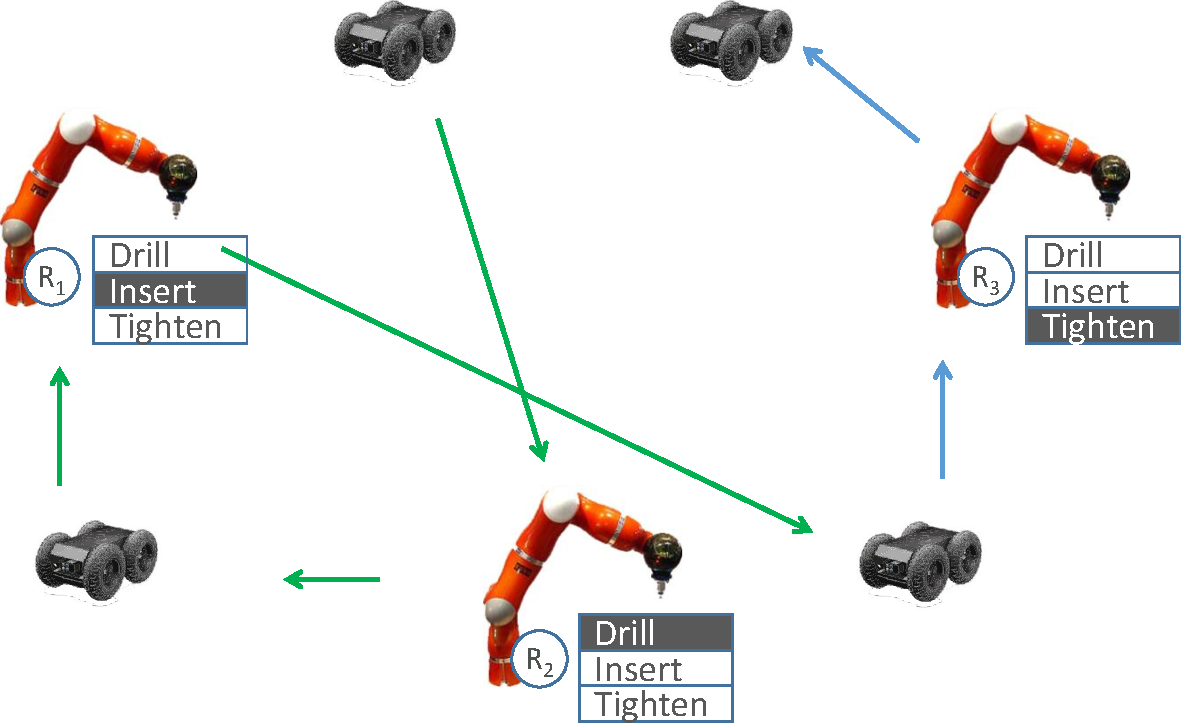
\includegraphics[width=.7\textwidth]{img/produktionszelle.pdf}
\end{center}

\hfill \cite{seebach2010software}

\end{frame}



\begin{frame}[fragile]
\frametitle{Constraint Satisfaction Probleme}

\vspace*{5ex}

\alert{Ziel:} Belege (endlich viele) Variablen aus $X$ mit einem aus (endlich vielen) Werten aus $D$ sodass alle Constraints $C$ erfüllt werden.

\vspace*{1ex}

\textbf{Beispiel}
\begin{itemize}
\item [-] $n$ Roboter, $m$ Tasks
\item [-] Gebe jedem Roboter einen \emph{unterschiedlichen} Task, stelle sicher, dass jeder Task belegt ist 
\end{itemize}

\begin{lstlisting}
% problem data 
int: n; set of int: ROBOTS = 1..n;
int: m; set of int: TASKS = 1..m;

% decisions
array[ROBOTS] of var TASKS: allocation;

% goal
solve satisfy;

% have robots work on different tasks
constraint alldifferent(allocation);
constraint forall(t in TASKS) (exists(r in ROBOTS) (allocation[r] = t));
\end{lstlisting}
\end{frame}

\begin{frame}[fragile]
\frametitle{Constraint Optimization Probleme}

\vspace*{4ex}

\alert{Ziel:} Suche die beste Belegung, sodass eine \textbf{skalare} Zielfunktion $f : [X \to D] \to \mathbb{Z}$ minimiert (oder maximiert) wird.

\vspace*{1ex}

\textbf{Beispiel}
\begin{itemize}
\item [-] $n$ (steuerbare) Supplier, $m$ (steuerbare) Consumer decken Residuallast
\end{itemize}

\begin{lstlisting}
% problem data 
int: n; set of int: SUPPLIERS = 1..n;
array[SUPPLIERS] of int: costs;
int: m; set of int: CONSUMERS = 1..m;
int: residualLoad;

% decisions
array[SUPPLIERS] of var 0..100: supply;
array[CONSUMERS] of var 0..100: demand;

% goal
solve minimize sum(s in SUPPLIERS)(costs[s]*supply[s]);

% have robots work on different tasks
constraint sum(supply) - sum(demand) - residualLoad = 0; 
\end{lstlisting}
\end{frame}

\begin{frame}{Energie: Nicht nur Hard Constraints}

\alert{Harte} Constraints aus Supply Automata:
\begin{equation}
\mathsf{hardBounds}: \forall t \in T, a \in A : m[a][t] = \mathsf{on} \rightarrow P_{\mathrm{min}} \leq S[a][t] \leq P_{\mathrm{max}} \nonumber
\end{equation}

\pause
\vspace*{2ex}
\alert{Weiche} Constraints anlagenspezifisch (z.B. Präferenz für 350 bis 390 KW):
\begin{equation}
\mathsf{ecoSweet}_{\mathsf{bio}}: \forall t \in T : m[\mathsf{biogas}][t] = \mathsf{on} \rightarrow 350 \leq S[\mathsf{biogas}][t] \leq 390 \nonumber
\end{equation}

\pause
\vspace*{2ex}
oder Änderungsgeschwindigkeit
\begin{equation}
\mathsf{inertia}_{\mathsf{therm}}: \forall t \in T : |S[\mathsf{biogas}][t] - S[\mathsf{biogas}][t+1] | \leq 10 \nonumber
\end{equation}
\end{frame}

\begin{frame}
    \frametitle{Soft Constraint Programming in MiniBrass}
 \alert{Constraint Programming}
    \begin{itemize}
    \item Deklarative Programmierung (ähnlich SQL, Prolog)
    \item Trennung von \textbf{Modell} und \emph{Algorithmus}
    \item Geeignet für kombinatorische Probleme unter harten Bedingungen (Physik!)
    \item Modellierungssprache \hFirst{MiniZinc}
    \end{itemize}

    \vspace*{3ex}
    
\alert{Soft Constraint Programming}
    \begin{itemize} 
    \item Modellierung von \textbf{Präferenzen}
    \item Finde Lösungen, die \emph{so gut wie möglich} sind
    \item Was bedeutet ``gut``?
    \item Modellierungssprache \hFirst{MiniBrass}
     \end{itemize}
\end{frame}


\begin{frame}{Warum MiniZinc?}
\begin{parchment}[Rationale]
\centering 
\alert{Eine Sprache -- viele Solver} 
\end{parchment}
\begin{textblock*}{2.cm}[1,1](\textwidth-.5cm,\textheight-1.03cm)


\includegraphics[width=\textwidth]{img/MiniZn_logo.jpg} 

\end{textblock*}
Unterstützte Solver
\begin{itemize}
\item Gecode (CP)
\item JaCoP (CP)
\item Google Optimization Tools (CP)
\item Choco (CP)
\item G12 (CP/LP/MIP)
\end{itemize}

\end{frame}

\tikzset{
   pvsNode/.style={rectangle, 
                   rounded corners,
                   minimum width=8cm,
                   minimum height=5cm,
                   draw,
                   dashed},
   sigNode/.style={rectangle, draw, solid},
   cpLogo/.style={fill=black,circle,minimum width=.5em},
   main node/.style={rectangle,
                     rounded corners,
   					 fill=black!15,
   					 draw,
   					 minimum width=3.5em,
   					 text centered,
                     inner sep=2.5pt,	 
   					 font=\sffamily\footnotesize
   					},
   weightNode/.style={rectangle,
                     rounded corners,
   					 fill=black,
   					 draw,
   					 minimum width=3.5em,
                     inner sep=2.5pt,	 
   					 font=\sffamily\footnotesize
   					}  					
}

\begin{frame}{Welche Arten von Soft Constraints?}

Was machen wir nun mit \alert{$\mathsf{inertia}_{\mathsf{therm}}$} und 
\alert{$\mathsf{ecoSweet}_{\mathsf{bio}}$}?
\begin{description}

\item[\textbf{Max-CSP}] Erfülle so viele Constraints wie möglich \hfill \hSecond{\cite{FreuderW92}} \pause 
\item[\textbf{Weighted CSP}] Minimiere die Summe der verletzten Constraints nach Gewicht \pause \hfill \hSecond{\cite{shapiro1981structural}}
\item[\textbf{Fuzzy CSP}] Erfülle den (minimalen) Erfüllungsgrad (zwischen 0 und 1) über alle Soft Constraints \hfill \hSecond{\cite{ruttkay1994fuzzy}} \pause 
\end{description} \pause 

\vspace*{1ex}

\ldots und natürlich 

\vspace*{1ex}

\begin{description}
\item[\textbf{Constraint Preferences}] (früher \emph{Constraint Relationships}): Definiere partielle Wichtigkeitsordnung über Constraints; erhebe diese zu Mengen von verletzten oder erfüllten Constraints \hfill \hFirst{\cite{Schiendorfer13}}
\end{description}

\vspace*{1ex}
\begin{parchment}[Zentrale Frage]
$\rightarrow$ Was sind die Gemeinsamkeiten? Was müssen wir ``minimal'' tun?
\end{parchment}
\end{frame}

\begin{frame}{Beispiel: Max-CSP}

\begin{figure}[t]
\centering
\begin{tikzpicture}[>=stealth',shorten >=1pt,anchor=north west] 


\begin{scope}
\node[pvsNode,minimum width=4cm,minimum height=3cm] (outer) at (0,0) {};

% the logo

\begin{scope}[node distance=.6cm]

\draw [shading=axis,bottom color=black!10,top color=white,rounded corners] (0,0) -- (0,-1) -- (1.3,-1) -- (1.7,0) -- (0,0);
\draw(0,-1) -- ($ (outer.north east) + (0,-1) $);


% weighted constraints%s logo
\node[cpLogo,scale=0.7,transform shape,] at (0.3,-.45) {};
\node[cpLogo,scale=0.7,transform shape,draw,fill=white] at (0.6,-.1) {};
\node[cpLogo,scale=0.7,transform shape,] at (0.4,-.75) {};
\node[cpLogo,scale=0.7,transform shape,draw] at (0.65,-.4) {};
\node[cpLogo,scale=0.7,transform shape,] at (0.3,-.45) {};
\node[cpLogo,scale=0.7,transform shape,draw,fill=white] at (0.9,-.6) {};

\node[cpLogo,scale=0.7,transform shape,] at (1.0,-.2) {};
\node[cpLogo,scale=0.7,transform shape,draw,fill=white] at (0.9,-.6) {};

\end{scope}

\node[main node,draw,anchor=west] (limitBu) at ($ (outer.center) + (-1,0.1)$)   {\limitBatteryUsage};

\node[main node, anchor=west, style={font=\sffamily\footnotesize}] (earlyBird) at ($(limitBu.west)+(-.9,-.8)$)  {\earlyBird};

\node[main node, anchor=west, style={font=\sffamily\footnotesize}] (prefBatteryLevel) at ($(limitBu.west)+(1.2,-.6)$)  {\prefBatteryLevel};


\end{scope}

\end{tikzpicture}
oder
\begin{tikzpicture}[>=stealth',shorten >=1pt,anchor=north west] 


\begin{scope}
\node[pvsNode,minimum width=4cm,minimum height=3cm] (outer) at (0,0) {};

% the logo

\begin{scope}[node distance=.6cm]

\draw [shading=axis,bottom color=black!10,top color=white,rounded corners] (0,0) -- (0,-1) -- (1.3,-1) -- (1.7,0) -- (0,0);
\draw(0,-1) -- ($ (outer.north east) + (0,-1) $);


% weighted constraints%s logo
\coordinate (beginLogo) at (0.4,0.0);
\node[cpLogo,anchor=south] (upLogo) at ($(beginLogo)+(0.3,-.45)$) {};

\draw [fill=black] ($(beginLogo)+(0,-.7)$) -- ($(beginLogo)+(0.1,-.4)$) -- ($(beginLogo)+(0.5,-.4)$) -- ($(beginLogo)+(0.6,-.7)$) -- ($(beginLogo)+(0,-.7)$);


\end{scope}

\node[weightNode,text=white,anchor=west,text width=1.5cm,text height=.19cm,align=right] (bg) at ($ (outer.center) + (-1,0.1)$)   {\hfill 78};
\node[main node,draw,anchor=west] (limitBu) at ($ (outer.center) + (-1,0.1)$)   {\limitBatteryUsage};

\node[weightNode,text=white,anchor=west,text width=1.75cm,text height=.19cm,align=right] (bg2) at ($(limitBu.west)+(0,-.5)$)   {\hfill 14};
\node[main node, anchor=west, style={font=\sffamily\footnotesize}] (earlyBird) at ($(limitBu.west)+(0,-.5)$)  {\earlyBird};

\node[weightNode,text=white,anchor=west,text width=1.3cm,text height=.19cm,align=right] (bg3) at ($(earlyBird.west)+(0,-.5)$)   {\hfill 3};
\node[main node, anchor=west, style={font=\sffamily\footnotesize}] (prefBatteryLevel) at ($(earlyBird.west)+(0,-.5)$)  {\prefBatteryLevel};


\end{scope}

\end{tikzpicture}

\vspace*{2ex}

oder 

\begin{tikzpicture}[>=stealth',shorten >=1pt,anchor=north west] 


\begin{scope}
\node[pvsNode,minimum width=4cm,minimum height=3cm] (outer) at (0,0) {};

% the logo

\begin{scope}[node distance=.6cm]

\draw [shading=axis,bottom color=black!10,top color=white,rounded corners] (0,0) -- (0,-1) -- (1.3,-1) -- (1.7,0) -- (0,0);
\draw(0,-1) -- ($ (outer.north east) + (0,-1) $);


% constraint relationship logo
\node[cpLogo] (upLogo) at (.55,-.2) {};
\node[cpLogo,below left of=upLogo] (leftLogo) {};
\node[cpLogo,below right of=upLogo] (rightLogo) {};  

\path[->]
  (leftLogo) edge node [right] {} (upLogo)
  (rightLogo) edge node [right] {} (upLogo)
;
\end{scope}

% spd parameter
\begin{scope}[node distance=.7cm,xshift=3cm,scale=.5,transform shape]

% constraint relationship logo
\node[fill,circle,OliveGreen] (upLogo) at ($ (outer.north east) + (-1.3,-0.2) $) {};
\node[fill,circle,BrickRed,below of=upLogo] (centerLogo) {};
\node[fill,circle,gray,left of=centerLogo] (leftLogo) {};
\node[fill,circle,gray,right of=centerLogo] (rightLogo) {};  
\node[below of=centerLogo,yshift=.4em,font=\Large] {$\mathrm{SPD}$};
\path[->]
  (leftLogo) edge node [right] {} (upLogo)
  (centerLogo) edge node [right] {} (upLogo)
  (rightLogo) edge node [right] {} (upLogo)
;

\end{scope}

% EV


\node[main node, anchor=center,style={font=\sffamily\footnotesize}] (8) at ($ (outer.center) + (0,-.8)$)   {\limitBatteryUsage};

\node[main node, style={font=\sffamily\footnotesize},above right of=8] (4)  {\earlyBird};

\node[main node, style={font=\sffamily\footnotesize},above left of=8] (3) {\prefBatteryLevel};

%\node[text width=2cm, anchor=west, left] at (4.3, 0.3) { CR };
%\node[text width=1cm, anchor=east, left] at (5.3, -2.3) { \textsc{SPD} };


\path[every node/.style={font=\sffamily\tiny},->]
  (8) edge node [right] {} (3)
  (8) edge node [right] {} (4)
;

\end{scope}

\end{tikzpicture}
\end{figure}
\end{frame}
\begin{frame}{Algebra zur Hilfe}

Wir benötigen \ldots 

\begin{itemize}
\item Eine Menge $M$ von Erfüllungsgraden, z.B. $[0.0, 1.0]$ oder $\{0, 1, \ldots k\}$ oder $2^{C_s}$. \pause 
\item Eine partielle Ordnung $\leq_M$ über $M$: $m \leq_M n$ drückt aus, dass $m$ \emph{schlechter} als $n$ ist \pause 
\item Eine Kombinationsoperation $\cdot_M$, um zwei Elemente aus $M$ miteinander zu verrechnen  \pause 
\item Ein bestes Element $\varepsilon_M$, um \emph{volle Zufriedenheit} auszudrücken \pause
\end{itemize}
  
  Gemeinsam nennen wir $(M, \cdot_M, \varepsilon_M, \leq_M)$ eine \textbf{partielle Bewertungsstruktur}.
  
  \hfill \emph{\cite{Gadducci2013,SchiendorferPvs2015}}
\end{frame}


%% block styles
\tikzstyle{sensor}=[draw, fill=blue!20, text width=5em, 
    text centered, minimum height=2.5em,drop shadow]    
    
\tikzstyle{alg} = [sensor, text width=5em, fill=isseorange!20, 
    minimum height=13em, rounded corners, drop shadow]
\tikzstyle{constraint}=[draw, circle, fill=issegrey!20, text width=1.2em, 
    text centered, minimum height=1.5em,drop shadow]
\tikzstyle{domainstore} = [alg, text width=5em, fill=isseorange!40, 
    minimum height=4em, rounded corners]
\tikzstyle{goodc} = [ForestGreen, font=\bfseries]
\tikzstyle{badc} = [Red, font=\bfseries]
\tikzstyle{okayc} = [LimeGreen, font=\bfseries]
        
\tikzset{
vecArrow/.style={
  thick
  }
}

\tikzset{
    mynode/.style={rectangle,rounded corners,draw=black, top color=isseorange!5, bottom color=isseorange!30,
                   very thick, inner sep=\myinnersep*1em, minimum size=3em, text centered, outer sep=0, align=center},
    innernode/.style={mynode, text width=3cm,  minimum height=1.5cm,
                      top color=issegrey!20, bottom color=issegrey!60},
    emphnode/.style={innernode, top color=isseorange!30, bottom color=isseorange!70}
}

% Define distances for bordering
\def\blockdist{2.3}
\def\edgedist{2.5}

  \tikzset{
    invisible/.style={opacity=0},
    visible on/.style={alt={#1{}{invisible}}},
    alt/.code args={<#1>#2#3}{%
      \alt<#1>{\pgfkeysalso{#2}}{\pgfkeysalso{#3}} % \pgfkeysalso doesn't change the path
    },
  }
%  
%\begin{frame}{Traditionelles Constraint-Solving}
%\fontsize{8pt}{7.2}\selectfont
%\begin{center}
%\begin{tikzpicture}
%% First row:
% \node (search) [alg]  {Suche \phantom{$x = 5$} };
% \path (search.east)+(4.6,0) node (propag) [alg,text width =12em]  {};
% \node[below right] at (propag.north west) {Constraint Store $C$};
% 
% \path (propag.west)+(0.8,-1.2) node (c1) [constraint] {$c_1$}; 
% \path (propag.west)+(1.1,-0.2) node (c2) [constraint] {$c_2$}; 
% \path (propag.west)+(2.0,0.4) node (c3) [constraint] {$c_3$}; 
% \path (propag.west)+(3.2,0.7) node (c4) [constraint] {$c_4$};
%  
% \path (propag.east)+(-1.2,-1.2) node (domainstore) [domainstore] {Domain Store $(D_x)_{x \in X}$}; 
% 
% \path [draw,vecArrow, ->] ([yshift=-2em]search.north east) -- node [above,visible on=<2->] {$x\gets5$} ([yshift=-2em]propag.north west);
% \path [draw,vecArrow, <-] ([yshift=2em]search.south east) -- node [above,goodc,visible on=<4->] {$\top$} ([yshift=2em]propag.south west);
% 
% \path [draw, vecArrow, <->] (c1.east) -- node [below,visible on=<3->,goodc] {$\top$} (domainstore.west) ;
% \path [draw,vecArrow, <->] (c2.330) -- node [above right,visible on=<3->,goodc] {$\top$} (domainstore.150) ;
% \path [draw,vecArrow, <->] (c3.290) -- node [right,visible on=<3->,goodc] {$\top$} (domainstore.120) ;
% \path [draw,vecArrow, <->] (c4.south) -- node [right,visible on=<3->,goodc] {$\top$} (domainstore.68) ;
%\end{tikzpicture}
%\end{center}
%\onslide<0>{
%\begin{columns}[c] % contents are top vertically aligned
%     \begin{column}[c]{7cm} % each column can also be its own 
%\begin{itemize}
%\item A set of satisfaction degrees $\mathbb{B} = \{ \bot, \top \}$
%\item A combination operation $\wedge$
%\item A neutral element $\top$
%\item A partial order $(\mathbb{B}, \leq_\mathbb{B})$ with $\top <_\mathbb{B} \bot$.
%\end{itemize}
%\end{column}
%     \begin{column}[c]{4.5cm} 
%     \end{column} 
%\end{columns}
%}
%
%\end{frame}
%
%\begin{frame}{Traditionelles Constraint-Solving}
%\fontsize{8pt}{7.2}\selectfont
%\begin{center}
%\begin{tikzpicture}
%% First row:
% \node (search) [alg]  {Suche $x = 5$};
% \path (search.east)+(4.6,0) node (propag) [alg,text width =12em]  {};
% \node[below right] at (propag.north west) {Constraint Store $C$};
% 
% \path (propag.west)+(0.8,-1.2) node (c1) [constraint] {$c_1$}; 
% \path (propag.west)+(1.1,-0.2) node (c2) [constraint] {$c_2$}; 
% \path (propag.west)+(2.0,0.4) node (c3) [constraint] {$c_3$}; 
% \path (propag.west)+(3.2,0.7) node (c4) [constraint] {$c_4$};
%  
% \path (propag.east)+(-1.2,-1.2) node (domainstore) [domainstore] {Domain Store $(D_x)_{x \in X}$}; 
% 
% \path [draw,vecArrow, ->] ([yshift=-2em]search.north east) -- node [above,visible on=<2->] {$y \gets 4$} ([yshift=-2em]propag.north west);
% \path [draw,vecArrow, <-] ([yshift=2em]search.south east) -- node [below,badc,visible on=<4->] {$\bot$} ([yshift=2em]propag.south west);
% 
% \path [draw, vecArrow, <->] (c1.east) -- node [below,visible on=<3->,badc] {$\bot$} (domainstore.west) ;
% \path [draw,vecArrow, <->] (c2.330) -- node [above right,visible on=<3->,goodc] {$\top$} (domainstore.150) ;
% \path [draw,vecArrow, <->] (c3.290) -- node [right,visible on=<3->,goodc] {$\top$} (domainstore.120) ;
% \path [draw,vecArrow, <->] (c4.south) -- node [right,visible on=<3->,goodc] {$\top$} (domainstore.68) ;
%\end{tikzpicture}
%\end{center}
%\onslide<5->{
%\begin{columns}[c] % contents are top vertically aligned
%     \begin{column}[c]{7cm} % each column can also be its own 
%\begin{itemize}
%
%\item Eine Menge von Bewertungen $\mathbb{B} = \{ \bot, \top \}$
%\item Eine Kombination $\wedge$
%\item Ein neutrales Element $\top$
%\item Eine partielle Ordnung $(\mathbb{B}, \leq_\mathbb{B})$ with $\top <_\mathbb{B} \bot$.
%\end{itemize}
%   \end{column} 
%     \begin{column}[c]{4.5cm} 
%     \end{column} 
%\end{columns}
%}
%\end{frame}

\begin{frame}{Soft-Constraint-Solving}
\fontsize{8pt}{7.2}\selectfont
\begin{center}
\begin{tikzpicture}
% First row:
 \node (search) [alg]  {Search $x = 5$};
 \path (search.east)+(4.6,0) node (propag) [alg,text width =12em]  {};
 \node[below right] at (propag.north west) {Constraint Store $C$};
 
 \path (propag.west)+(0.8,-1.2) node (c1) [constraint] {$c_1$}; 
 \path (propag.west)+(1.1,-0.2) node (c2) [constraint] {$c_2$}; 
 \path (propag.west)+(2.0,0.4) node (c3) [constraint] {$c_3$}; 
 \path (propag.west)+(3.2,0.7) node (c4) [constraint] {$c_4$};
  
 \path (propag.east)+(-1.2,-1.2) node (domainstore) [domainstore] {Domain Store $(D_x)_{x \in X}$}; 
 
 \path [draw,vecArrow, ->] ([yshift=-2em]search.north east) -- node [above,visible on=<2->] {$y \gets 4$} ([yshift=-2em]propag.north west);
 \path [draw,vecArrow, <-] ([yshift=2em]search.south east) -- node [below,okayc,visible on=<4->] {$4$} ([yshift=2em]propag.south west);
 
 \path [draw, vecArrow, <->] (c1.east) -- node [below,visible on=<3->,okayc] {$4$} (domainstore.west) ;
 \path [draw,vecArrow, <->] (c2.330) -- node [above right,visible on=<3->,goodc] {$0$} (domainstore.150) ;
 \path [draw,vecArrow, <->] (c3.290) -- node [right,visible on=<3->,goodc] {$0$} (domainstore.120) ;
 \path [draw,vecArrow, <->] (c4.south) -- node [right,visible on=<3->,goodc] {$0$} (domainstore.68) ;
\end{tikzpicture}
\end{center}
\onslide<5->{
\begin{columns}[c] % contents are top vertically aligned
     \begin{column}[c]{7cm} % each column can also be its own environment
    \begin{itemize}
\item Eine Menge von Bewertungen, z.B., $\{ 0, \ldots, k \}$
\item Eine Kombination $+$
\item Ein neutrales Element $0$
\item Eine partielle Ordnung $(\mathbb{N}, \geq)$ mit $0$ als Top 
\end{itemize}
   \end{column} \pause
     \begin{column}[c]{4.5cm} 
        Genannt \cemph{valuation structure}~\cite{Schiex1995valued}, bei totaler Ordnung, ansonsten \cemph{partial valuation structure}~\cite{Gadducci2013}.
        Ähnlich:  \cite{Bistarelli1999}: c-Semiringe 
     \end{column}
\end{columns}
    
}
\end{frame}


\begin{frame}[fragile]{PVS--Idee}
\begin{center}
\begin{tabular}{l|c|c|c|c}
\textbf{Konkrete PVS-Typen} & $M$ & $\cdot_M$ & $\leq_M$ & $\varepsilon_M$ \\ 
\hline 
Weighted CSP (WCSP)& $\mathbb{N}$ & $+$ & $\geq$ & $0$ \\ 
Cost Function Network (CFN)& $\{0,\ldots,k\}$ & $+$/$\max$ & $\geq$ & $0$ \\ 
Fuzzy CSP & $[0,1]$ & $\min$ & $\leq$  & 1 \\ 
Inclusion Max CSP & $2^{C_s}$ & $\cup$ & $\supseteq$  & $\emptyset$ \\ 
Constraint Preferences (CP)\footnote{$C_s$ is the set of soft constraints, $\supseteq_{\mathsf{SPD}}$ is the SPD-ordering on sets.} &$\mathcal{M}^{\mathrm{fin}} (C_s)$ & $\mcup$ & $\supseteq_{\mathsf{SPD}}$ & $\lbag \rbag$ \\ 
\end{tabular} 
\end{center}

\begin{parchment}[Hauptidee]
Implementiere Lösungsverfahren für Constraint-Probleme, die durch Bewertungsstrukturen geordnet sind. Instantiiere für konkrete Probleme.
\end{parchment}
\end{frame}

\begin{frame}{Kombinationen~\cite{SchiendorferPvs2015}}
\begin{tikzpicture}[>=stealth',shorten >=1pt,anchor=north west] 

%% FIRST OVERALL LAYER 

\draw[CornflowerBlue,thick,fill=white] (-0.4,2.95) rectangle (11.7,-5.1);
\node[CornflowerBlue] at (0, 2.9) {$\ltimes \quad \mathtt{lex}$};
\draw[CornflowerBlue,thick] (-0.4,1) -- (11.7,1);

% the logo

\begin{scope}[yshift=2.45cm]

\node[pvsNode,minimum width=11.5cm,minimum height=1.5cm] (outer) at (0,0) {};


\begin{scope}[node distance=.6cm]

\draw [shading=axis,bottom color=black!10,top color=white,rounded corners] (0,0) -- (0,-1) -- (1.3,-1) -- (1.7,0) -- (0,0);
\draw(0,-1) -- ($ (outer.north east) + (0,-1) $);


% cost function networks logo

\node at (.1,-.3) {\Huge \EUR};
\node at (.6,-0.1) {\Large $\mathbb{Z}$};

\end{scope}

% spd parameter
\begin{scope}[node distance=.7cm,xshift=1.7cm,scale=.5,transform shape]

% cfn logos
\draw[thick,->] ($(outer.east) + (-1.3,1.4)$) -- ($(outer.east) + (-1.3,0.6)$);
\node[font=\Large,anchor=east] at ($(outer.east) + (-0.5,0.3)$) {$\mathrm{Minimize}$};


\node[font=\Huge,anchor=east] at ($(outer.east) + (-2.7,1.1)$) {$\mathrm{\max}$};
\node[font=\Large,anchor=east] at ($(outer.east) + (-2.7,0.3)$) {$\mathrm{Maximum}$};

\end{scope}

\node[ anchor=center] at  ($ (outer.center) + (0.2,.1)$) {  $\mathtt{\biogas1}$ };
% EV
\begin{scope}[node distance = 1.5cm]

\node[main node, anchor=center,style={font=\sffamily\footnotesize}] (cm) at ($ (outer.center) + (-0.6,-0.5)$)   {$\mathtt{costsMaint}$};

\node[main node, style={font=\sffamily\footnotesize},right of=cm] (cf)  {$\mathtt{costsFuel}$};
\end{scope}

%\node[text width=2cm, anchor=west, left] at (4.3, 0.3) { CR };
%\node[text width=1cm, anchor=east, left] at (5.3, -2.3) { \textsc{SPD} };


\end{scope}

\begin{scope}
\node[pvsNode,minimum width=4cm,minimum height=3cm] (outer) at (0,0) {};

% the logo
\draw[isseorange,thick] (-0.2,0.7) rectangle (11.6,-5);
\draw[isseorange,thick,dotted] (4.5,0.7) -- (4.5,-5);
\node[isseorange] at (0, 0.7) {$\times \quad \mathtt{pareto}$};

\begin{scope}[node distance=.6cm]

\draw [shading=axis,bottom color=black!10,top color=white,rounded corners] (0,0) -- (0,-1) -- (1.3,-1) -- (1.7,0) -- (0,0);
\draw(0,-1) -- ($ (outer.north east) + (0,-1) $);


% constraint relationship logo
\node[cpLogo] (upLogo) at (.55,-.2) {};
\node[cpLogo,below left of=upLogo] (leftLogo) {};
\node[cpLogo,below right of=upLogo] (rightLogo) {};  

\path[->]
  (leftLogo) edge node [right] {} (upLogo)
  (rightLogo) edge node [right] {} (upLogo)
;
\end{scope}

% spd parameter
\begin{scope}[node distance=.7cm,xshift=3cm,scale=.5,transform shape]

% constraint relationship logo
\node[fill,circle,OliveGreen] (upLogo) at ($ (outer.north east) + (-1.3,-0.2) $) {};
\node[fill,circle,BrickRed,below of=upLogo] (centerLogo) {};
\node[fill,circle,gray,left of=centerLogo] (leftLogo) {};
\node[fill,circle,gray,right of=centerLogo] (rightLogo) {};  
\node[below of=centerLogo,yshift=.4em,font=\Large] {$\mathrm{SPD}$};
\path[->]
  (leftLogo) edge node [right] {} (upLogo)
  (centerLogo) edge node [right] {} (upLogo)
  (rightLogo) edge node [right] {} (upLogo)
;
\end{scope}

% EV

\node[ anchor=center] at  ($ (outer.center) + (0.2,.7)$) {  $\mathtt{\ev}$ };



\node[main node, anchor=center,style={font=\sffamily\footnotesize}] (8) at ($ (outer.center) + (0,-.8)$)   {\limitBatteryUsage};

\node[main node, style={font=\sffamily\footnotesize},above right of=8] (4)  {\earlyBird};

\node[main node, style={font=\sffamily\footnotesize},above left of=8] (3) {\prefBatteryLevel};

%\node[text width=2cm, anchor=west, left] at (4.3, 0.3) { CR };
%\node[text width=1cm, anchor=east, left] at (5.3, -2.3) { \textsc{SPD} };


\path[every node/.style={font=\sffamily\tiny},->]
  (8) edge node [right] {} (3)
  (8) edge node [right] {} (4)
;

\end{scope}


%% SECOND PVS 
%%%%%%%%%%%%%%%%%%%
% First Layer
\begin{scope}[xshift=5.2cm]
\node[pvsNode,minimum width=6cm,minimum height=1.8cm] (outer) at (0,0) {};

\draw[CornflowerBlue,thick] (-0.2,0.5) rectangle (6.2,-4.9);
\draw[CornflowerBlue,thick] (-0.2,-2) -- (6.2,-2);
\node[CornflowerBlue] at (0, 0.5) {$\ltimes \quad \mathtt{lex}$};
% the logo

\begin{scope}[node distance=.6cm]

\draw [shading=axis,bottom color=black!10,top color=white,rounded corners] (0,0) -- (0,-1) -- (1.3,-1) -- (1.7,0) -- (0,0);
\draw(0,-1) -- ($ (outer.north east) + (0,-1) $);


% cost function networks logo

\node at (.1,-.3) {\Huge \EUR};
\node at (.6,-0.1) {\Large $\mathbb{Z}$};

\end{scope}

% spd parameter
\begin{scope}[node distance=.7cm,xshift=1.7cm,scale=.5,transform shape]

% cfn logos
\draw[thick,<-] ($(outer.east) + (-1.3,1.4)$) -- ($(outer.east) + (-1.3,0.6)$);
\node[font=\Large,anchor=east] at ($(outer.east) + (-0.5,0.3)$) {$\mathrm{Maximize}$};


\node[font=\Huge,anchor=east] at ($(outer.east) + (-2.7,1.1)$) {$\mathrm{\sum}$};
\node[font=\Large,anchor=east] at ($(outer.east) + (-2.7,0.3)$) {$\mathrm{Sum}$};

\end{scope}

\node[ anchor=center] at  ($ (outer.center) + (0.2,.1)$) {  $\mathtt{\biogas1}$ };
% EV
\begin{scope}[node distance = 1.5cm]

\node[main node, anchor=center,style={font=\sffamily\footnotesize}] (cm) at ($ (outer.center) + (-0.6,-0.5)$)   {$\mathtt{costsMaint}$};

\node[main node, style={font=\sffamily\footnotesize},right of=cm] (cf)  {$\mathtt{costsFuel}$};
\end{scope}

%\node[text width=2cm, anchor=west, left] at (4.3, 0.3) { CR };
%\node[text width=1cm, anchor=east, left] at (5.3, -2.3) { \textsc{SPD} };


\end{scope}

%% SECOND LAYER 
\begin{scope}[xshift=5.2cm,yshift=-2.3cm]
\node[pvsNode,minimum width=6cm,minimum height=2.5cm] (outer) at (0,0) {};

% the logo

\begin{scope}[node distance=.6cm]

\draw [shading=axis,bottom color=black!10,top color=white,rounded corners] (0,0) -- (0,-1) -- (1.3,-1) -- (1.7,0) -- (0,0);
\draw(0,-1) -- ($ (outer.north east) + (0,-1) $);


% constraint relationship logo
\node[cpLogo] (upLogo) at (.55,-.2) {};
\node[cpLogo,below left of=upLogo] (leftLogo) {};
\node[cpLogo,below right of=upLogo] (rightLogo) {};  

\path[->]
  (leftLogo) edge node [right] {} (upLogo)
  (rightLogo) edge node [right] {} (upLogo)
;
\end{scope}

% spd parameter
\begin{scope}[node distance=.7cm,xshift=3cm,scale=.5,transform shape]

% constraint relationship logo
\node[fill,circle,OliveGreen] (upLogo) at ($ (outer.north east) + (-1.3,-0.2) $) {};
\node[fill,circle,BrickRed,below of=upLogo] (centerLogo) {};
\node[fill,circle,BrickRed,left of=centerLogo] (leftLogo) {};
\node[fill,circle,BrickRed,right of=centerLogo] (rightLogo) {};  
\node[below of=centerLogo,yshift=.4em,font=\Large] {$\mathrm{TPD}$};
\path[->]
  (leftLogo) edge node [right] {} (upLogo)
  (centerLogo) edge node [right] {} (upLogo)
  (rightLogo) edge node [right] {} (upLogo)
;

\end{scope}

% BIOGAS Plant 
\begin{scope}[node distance =1.2cm]
\node[main node, anchor=center, style={font=\sffamily\footnotesize}] (gf) at ($ (outer.center) + (0,0)$) {\gasFull};
\node[main node, style={font=\sffamily\footnotesize}] (ecs) [below left of=gf,xshift=5.4] {\ecoSweet};
\node[main node, style={font=\sffamily\footnotesize}] (ono) [below right of=gf,xshift=-3.1] {\onOff};
\end{scope}
%\node[main node, style={font=\sffamily\footnotesize},double] (hardConstraint) [below left of=7,xshift=-3.1,yshift=7] {$\mathsf{maxProd}$};
\node[ anchor=center] at  ($ (outer.center) + (0.2,.7)$) {  $\mathtt{\biogas2}$ };


%\node[text width=2cm, anchor=west, left] at (4.3, 0.3) { CR };
%\node[text width=1cm, anchor=east, left] at (5.3, -2.3) { \textsc{SPD} };


\path[every node/.style={font=\sffamily\tiny},->]
  (ono) edge node [right] {} (gf)
  (ecs) edge node [right] {} (gf)
;

\end{scope}
\end{tikzpicture}
\end{frame}

\begin{frame}{Kombinationen~\cite{SchiendorferPvs2015}}
\fontsize{8pt}{7.2}\selectfont
\tikzset{
   main node/.style={rectangle,
                     rounded corners,
   					 fill=black!15,
   					 draw,
   					 minimum width=3.5em,
   					 text centered,
                     inner sep=2.5pt,	 
   					 font=\sffamily
   					},
   treestyle/.style={rectangle,fill=black!15,draw,font=\sffamily},
   constraint/.style={circle,fill=black!15,draw,font=\sffamily\small},
   constraint_satisfied/.style = {constraint, fill=white},
   constraint_violated/.style = {constraint, fill=black!25},
}

\begin{figure}[t]
\centering
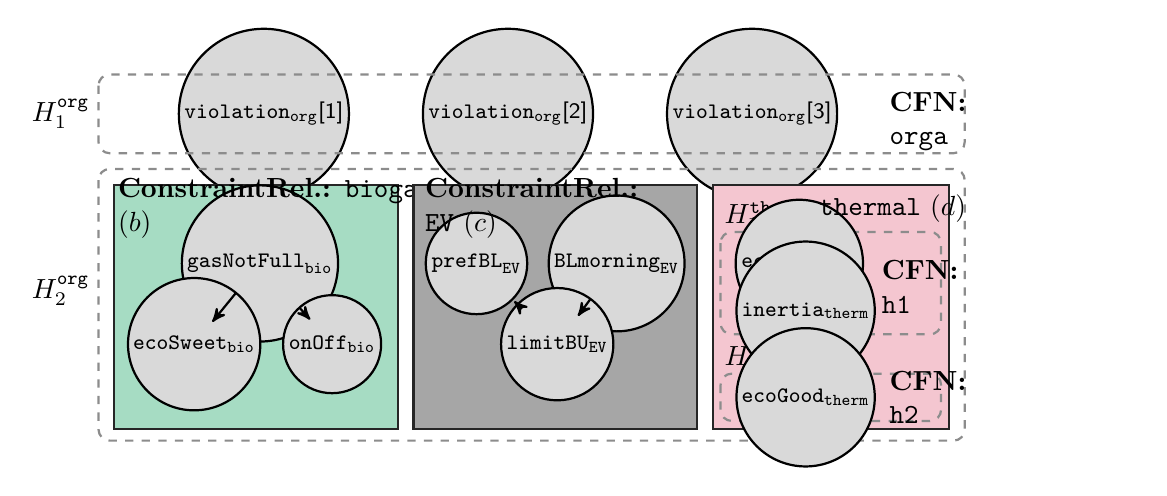
\begin{tikzpicture}[->,>=stealth',shorten >=1pt,auto,node distance=1.45cm,inner sep=1.5pt,outer sep = 0.0pt, thick] 
%\tikzstyle{every node}=[font=\tiny]
\begin{scope}[xshift=-6.0cm,yshift=-4.0cm]
\node[main node, style={font=\sffamily\footnotesize}] at (0.1,1.5) {\minMaxViolation[1]};
\node[main node, style={font=\sffamily\footnotesize}] at (3.2,1.5) {\minMaxViolation[2]};
\node[main node, style={font=\sffamily\footnotesize}] at (6.3,1.5) {\minMaxViolation[3]};

\draw [rounded corners,dashed,black!45] (-2,2) rectangle (9.0,1);
\node[text width=3cm, anchor=west, right] at (-2.9, 1.5) { \hLevelOrg{1} };
\draw [rounded corners,dashed,black!45] (-2,0.8) rectangle (9.0,-2.65);
\node[text width=4cm, anchor=west, right] at (-2.9, -0.75) { \hLevelOrg{2} };

% bio
\draw [black!85,fill=forestgreen!35] (-1.8,0.6) rectangle (1.8,-2.5);
\node[main node, style={font=\sffamily\footnotesize}] (5) at (0.05,-0.4) {\gasFull};
\node[main node, style={font=\sffamily\footnotesize}] (6) [below left of=5,xshift=5.4] {\ecoSweet};
\node[main node, style={font=\sffamily\footnotesize}] (7) [below right of=5,xshift=-3.1] {\onOff};
%\node[main node, style={font=\sffamily\footnotesize},double] (hardConstraint) [below left of=7,xshift=-3.1,yshift=7] {$\mathsf{maxProd}$};
\node[text width=4cm, anchor=west, left] at (2.3, 0.3) { \textbf{ConstraintRel.:}  $\mathtt{\biogas}$ $(b)$ };
%\node[text width=2cm, anchor=west, left] at (0.4, 0.3) { CR \textsc{TPD} };

% EV
\draw [black!85,fill=black!35] (2.0,0.6) rectangle (5.6,-2.5);
\node[main node, style={font=\sffamily\footnotesize}] (3) at (2.80,-0.4) {\prefBatteryLevel};
\node[main node, style={font=\sffamily\footnotesize}] (4) at (4.58,-0.4)  {\earlyBird};
\node[main node, style={font=\sffamily\footnotesize}] (8) [below right of=3] {\limitBatteryUsage};
\node[text width=3cm, anchor=west, left] at (5.2, 0.3) { \textbf{ConstraintRel.:}  $\mathtt{\ev}$ $(c)$ };
%\node[text width=2cm, anchor=west, left] at (4.3, 0.3) { CR };
%\node[text width=1cm, anchor=east, left] at (5.3, -2.3) { \textsc{SPD} };

% thermal
\draw [black!85,fill=thermicred!25] (5.8,0.6) rectangle (8.8,-2.5);
\draw [rounded corners,dashed,black!45] (5.9,0) rectangle (8.7,-1.3);
\node[text width=4cm, anchor=west, right] at (5.9, 0.2) { \hLevelThermal{1} };
\draw [rounded corners,dashed,black!45] (5.9,-1.8) rectangle (8.7,-2.4);
\node[text width=4cm, anchor=west, right] at (5.9, -1.6) { \hLevelThermal{2} };
\node[main node, style={font=\ttfamily\footnotesize}] (10) at (6.9,-0.4) {\ecoOpt};
\node[main node, node distance=0.85cm, style={font=\sffamily\footnotesize}] (11) at (6.98,-1.0) {\inertia};
\node[main node, node distance=0.85cm, style={font=\sffamily\footnotesize}] (12) at (6.98,-2.1) {\ecoGood};
\node[text width=4cm, anchor=west, right] at (7.1, 0.3) { $\mathtt{\thermal}$ $(d)$ };

\node[text width=2cm, anchor=west, left] at (10, -0.7) { \textbf{CFN:} \\ $\mathtt{h1}$ };

\node[text width=2cm, anchor=west, left] at (10.1, -2.1) { \textbf{CFN:} \\ $\mathtt{h2}$ };

\node[text width=2cm, anchor=west, left] at (10.1, 1.4) { \textbf{CFN:} \\ $\mathtt{orga}$ };

\path[every node/.style={font=\sffamily\tiny}]
  (8) edge node [right] {} (3)
  (8) edge node [right] {} (4)
  (6) edge node [right] {} (5)
  (7) edge node [right] {} (5)
;
\end{scope}

% \begin{scope}[xshift=-0.2cm,yshift=-0.9cm]
% \node[text width=9cm,left] at (0.0, 0.0) {%
% \begin{itemize}[itemsep=2pt]
%   \item something interesting
% \end{itemize}
% };
% \end{scope}

\end{tikzpicture}
%\caption{Case study depicting individual and organizational preference specifications in context.}
\label{fig:preferencesCaseStudy}
\end{figure}
  



%%% Local Variables:
%%% mode: LaTeX
%%% mode: TeX-PDF
%%% mode: TeX-source-correlate
%%% TeX-master: "../quality-quantity-soft-constraints.tex"
%%% End:


\onslide<2->{
Die Bewertungsstruktur dieses Problems:
\vspace*{2ex}

\qquad $
  P_{\mathtt{org}_1} \ltimes (P_{\prosumer{\biogas}} \times P_{\prosumer{\ev}} \times (P_{\prosumer{\thermal}}^1 \ltimes P_{\prosumer{\thermal}}^2))
$
}
%
%\begin{textblock*}{7.5cm}[1,1](\textwidth+3.8cm,\textheight-0.13cm)
%\begin{itemize}
%%\item[] \textsc{SPD} \ldots Single-Pred.-Dom.
%%\item[] \textsc{TPD} \ldots Single-Pred.-Dom.
%\item[] \textsc{SUM} \ldots Sum of Errors
%\item[] \textsc{WC} \ldots Worst-Case Error
%
%
%\end{itemize}
% \end{textblock*}
\end{frame}


\begin{frame}{Was müssen wir mindestens tun?}
\newcolumntype{C}[1]{>{\centering\let\newline\\\arraybackslash\hspace{0pt}}m{#1}}
\begin{tikzpicture}[->,>=stealth',shorten >=1pt,
  thick,main node/.style={circle,inner sep=1.5pt,fill=black!15,draw,font=\sffamily}, scale=1.15,
   pvs/.style={shape=rectangle, rounded corners,draw=issegrey!50,align=center}]
%%%%%%%%%%%%%%%%%% Orderings and embeddings

\node (t) at (4.3,6.5) {{$\top$}};
\node [text width=2.4cm](labelR) at ($(t)+(1,.7)$) {$\mathsf{P}$};

\node (r2) at ($(t)-(0.5,1)$) {{$\RN{2}$}};
\node (a2) at ($(t)-(-0.5,1)$) {{$2$}};

\node (r1) at ($(r2)-(0,1)$) {{$\RN{1}$}};
\node (a1) at ($(a2)-(0,1)$) {{$1$}};


\path[-,thin]
(r1) edge (r2)
     edge (a2)
(a1) edge (r2)
     edge (a2)
(a2) edge (t)
(r2) edge (t)
;      

  
   

%%%%%%%%%%%%%%%%%% SCSP problem
  \node[main node,minimum size = 12pt,text depth=.25ex,anchor=west,label=west:] (x) at (0,3) {$x$} ;
  \node[main node,minimum size = 12pt,text depth=.25ex,label=west:] (y) at ($(x)+(4.5,0)$) {$y$};  
  \node[main node,minimum size = 12pt,text depth=.25ex,label=east:] (z) at ($(x)+(9,0)$) {$z$};  
  \node[anchor=north west] (scsplabel) at ($(x)+(-.5,.7)$) {\color{issegrey} $SCSP$};

\node[pvs,dotted,text width=11.85cm,anchor=north west, text height=3.4cm] at ($(scsplabel.north west)+(-.3,0)$) {};
  \path[-,thin]
    (x) edge (y)
    (y) edge (z)
  ;
  \draw [thin,densely dashed,-] (x.south) -- ( $ (x.south) + (0,-.45)$); 
  \draw [thin,densely dashed,-] (y.south) -- ( $ (y.south) + (0,-.45)$);
  \draw [thin,densely dashed,-] (z.south) -- ( $ (z.south) + (0,-.45)$);   
  
  \node[anchor=north] (mux) at ($(x)+(0,-.5)$) {
\begin{tabular}{|c|c|}
  \hline 
  $x$ & $\mu_x$ \\ 
  \hline 
  0 & 1 \\ 
  1 & 2 \\ 
  \hline 
  \end{tabular}   
  };  
  
  \node[anchor=north] (muy) at ($(y)+(0,-.5)$) {
\begin{tabular}{|c|c|}
  \hline 
  $y$ & $\mu_y$ \\ 
  \hline 
  0 & 1 \\ 
  1 & 2 \\ 
  \hline 
  \end{tabular}   
  };  
  
    \node[anchor=north] (muz) at ($(z)+(0,-.5)$) {
\begin{tabular}{|c|c|}
  \hline 
  $z$ & $\mu_z$ \\ 
  \hline 
  0 & $\RN{2}$ \\ 
  1 & 1 \\ 
  \hline 
  \end{tabular}   
  };  
  
    \node[anchor=north] (muyx) at ($(x)+(2.25,-.5)$) {
\begin{tabular}{|c|c|c|}
  \hline 
  $x$ & $y$ & $\mu_{xy}$ \\ 
  \hline 
  0 & 0 & $\top$\\ 
  0 & 1 & $\RN{2}$\\ 
  1 & 0 & 2\\ 
  1 & 1 & 1\\  
  \hline 
  \end{tabular}   
  };  

    \node[anchor=north] (muyz) at ($(y)+(2.25,-.5)$) {
\begin{tabular}{|c|c|c|}
   \hline 
  $y$ & $z$ & $\mu_{yz}$ \\ 
  \hline 
  0 & 0 & $\RN{2}$\\ 
  0 & 1 & $\RN{1}$\\ 
  1 & 0 & $2$\\ 
  1 & 1 & 1\\ 
  \hline 
  \end{tabular}   
  };    
  
  \draw [thin,densely dashed,-] ($(muyx.north)+(0,.5)$) -- ($(muyx.north)+(0,-0.1)$);  
  
  \draw [thin,densely dashed,-] ($(muyz.north)+(0,.5)$) -- ($(muyz.north)+(0,-0.1)$);  
%\node[anchor=west] at (-.7, -3.5) { \textbf{Elimination order}:$\langle x, y, z \rangle$};

% |x| = \twopartdef { x } {x \geq 0} {-x} {x < 0}
%\node[anchor=west] at (-.7, -3.8) {\textbf{Embedding } into $\cSRngfree{\mathsf{R}}$: };

\end{tikzpicture}

\end{frame}

\begin{frame}{Von POs zu PVS: Skizze}

{
\Large
\begin{itemize}
\item Angenommen $(P, \leq_P)$ \pause 
\item Wir suchen eine PVS $(M, \cdot_M, \varepsilon_M, \leq_M)$ \pause
\item Wie \alert{Multiplikation} konstruieren?
\begin{itemize}
\item[-] Repräsentiere $p \in P$ durch ``sich selbst'': $p \in M$ $\checkmark$ \pause 
\item[-] Füge neue Elemente ``$p \cdot_M q$'' für alle Elemente $p,q \in M$ aus $\checkmark$ \pause
\item[-] Stelle sicher dass Kommutativität und Assoziativität gelten, nicht aber \emph{Idempotenz}: $(p \cdot_M q) \cdot_M r  = q \cdot_M (r \cdot_M p)$   \pause
\item[-] $\rightarrow$ Wähle \emph{Multimengen} über $P$ als Repräsentant der Produkte aus (Mengen \emph{wären} idempotent: $p \cdot_M p \neq p$ soll aber gelten. \pause
\item[-] Neutrales Element $\lbag \rbag$ für Multiplikation ``geschenkt''
\end{itemize}
\vspace*{2ex}
\pause
\item Welche Ordnungsbeziehungen \emph{müssen} gelten? \pause
\begin{itemize}
\item[-] Wenn $p \leq_P q$ dann $\lbag p \rbag \smytheq{P} \lbag q \rbag$ 
\item[-] $X \smytheq{P} \lbag  \rbag$, weil $\varepsilon_M$ das Maximum in $\leq_M$ sein soll
\item[-] Genannt: \alert{Smyth-Ordnung}
\end{itemize}
\item Beispiel: $\lbag 1, \RN{1}, 2 \rbag \smytheq{P} \lbag 2, \RN{2} \rbag$
\end{itemize}
}
\end{frame}

\begin{frame}{Was müssen wir mindestens tun?}

\begin{center} 
\newcolumntype{C}[1]{>{\centering\let\newline\\\arraybackslash\hspace{0pt}}m{#1}}
\begin{tikzpicture}[->,>=stealth',shorten >=1pt,
  thick,main node/.style={circle,inner sep=1.5pt,fill=black!15,draw,font=\sffamily}, scale=1.15,
   pvs/.style={shape=rectangle, rounded corners,draw=issegrey!50,align=center}]
%%%%%%%%%%%%%%%%%% Orderings and embeddings

\node (t) at (0.3,6.5) {{$\top$}};
\node [text width=2.4cm](labelR) at ($(t)+(1,.7)$) {$\mathsf{R}$};

\node (r2) at ($(t)-(0.5,1)$) {{$\RN{2}$}};
\node (a2) at ($(t)-(-0.5,1)$) {{$2$}};

\node (r1) at ($(r2)-(0,1)$) {{$\RN{1}$}};
\node (a1) at ($(a2)-(0,1)$) {{$1$}};


\path[-,thin]
(r1) edge (r2)
     edge (a2)
(a1) edge (r2)
     edge (a2)
(a2) edge (t)
(r2) edge (t)
;      

\draw [thin,dashed,-] ($(t)+(1.2,.5)$) -- ($(t)+(1.2,-5.5)$);
  
 % PVS<R>

\node [anchor=west,text width=5cm](labelPV) at ($(t)+(2.7,0.7)$) {$\PVSfree{\mathsf{R}}$};

\node (peps) at ($(t)+(3.25,0)$) {\color{isseorange} $\lbag \rbag$};
\node (pt) at ($(peps)-(0,1)$) {{$\lbag \top \rbag$}};
\node (pr2) at ($(pt)-(0.5,1)$) {{$\lbag \RN{2} \rbag$}};
\node (pa2) at ($(pt)-(-0.5,1)$) {{$\lbag 2 \rbag$}};

\node (pr1) at ($(pr2)-(0,1)$) {{$\lbag \RN{1} \rbag$}};
\node (pa1) at ($(pa2)-(0,1)$) {{$\lbag 1 \rbag$}};

\node (pr11) at ($(pr1)-(0,1)$) {\color{isseorange} $\lbag 1, \RN{1} \rbag$};
\node (pa11) at ($(pa1)-(0,1)$) {\color{isseorange} $\lbag 1, \RN{2} \rbag$};

\node (leftdots) at ($(pr1)-(1,1)$) {{\ldots}};
\node (rightdots) at ($(pa1)-(-1,1)$) {{\ldots}};

\node (downdots1) at ($(pr11)-(0,.75)$) {{\ldots}};
\node (downdots2) at ($(pa11)-(0,.75)$) {{\ldots}};

\path[-,thin]
(pr1) edge (pr2)
     edge (pa2)
(pa1) edge (pr2)
     edge (pa2)
(pa2) edge (pt)
(pr2) edge (pt)
(pt) edge (peps)
(pa11) edge (pa1)
(pr11) edge (pa1)
(pr11) edge (pr1)
(leftdots) edge (pr1)
(rightdots) edge (pa1)
(downdots1) edge (pr11)
(downdots2) edge (pa11)
;    
   
\end{tikzpicture}

\end{center}
\end{frame}



\begin{frame}{Looking for freedom \ldots} \small

\begin{center}
\begin{tikzpicture}[auto,->,
                    >=stealth',shorten >=1pt,thick,
                    node distance=.7cm,inner sep=2pt,
                    constraint/.style={circle,fill=black!15,draw,font=\sffamily\small},
                    bg/.style={shape=rectangle, rounded corners,
    draw, align=center,
    top color=white, bottom color=issegrey!15},
                    pvs/.style={shape=rectangle, rounded corners,
    draw=isseorange!50,fill=white, align=center}]
\node [anchor=west] at (0, .5) {$\mathrm{Cat}: \mathrm{POSet}$};
\node [anchor=west] at (0, -.5) {$\mathrm{Cat}: \mathrm{PVS}$};

\draw [dashed,-] (0,0) -- (11,0);

 \node[bg,text width=2.7cm, text height=1.5cm] at (5,1.6) {};
 \node[anchor=west] at (3.6,2.1) {$P$};
 
\node[constraint] (1) at (5, 2)                   {$\mathrm{c}_1$};
\node[constraint] (2) at ($ (1) + (-0.8, -0.8) $) {$\mathrm{c}_2$};  
\node[constraint] (3) at ($ (1) + ( 0.8, -0.8) $) {$\mathrm{c}_3$};  
%  
\path[every node/.style={font=\sffamily\tiny}]
  (2) edge (1)
  (3) edge (1)
  ;
 
\onslide<2-> { 
\node[pvs,text width=3.5cm,anchor=north west, text height=2.8cm] at (0.5,-1) {};
 \node[anchor=west] at (0.5,-1.3) {$\mathit{Weighted}(P)$};
  \node[anchor=west] at (0.5,-3.6) {$\langle \mathbb{N}, +, \geq, 0 \rangle$};
  
\node[constraint,label=west:2] (w1) at (2, -2)                   {$\mathrm{c}_1$};
\node[constraint,label=west:1] (w2) at ($ (w1) + (-0.8, -0.8) $) {$\mathrm{c}_2$};  
\node[constraint,label=west:1] (w3) at ($ (w1) + ( 0.8, -0.8) $) {$\mathrm{c}_3$};  
\node at (3.5, -2.3) {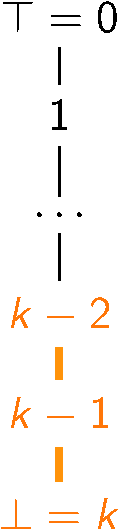
\includegraphics[width=.45cm]{img/search-space-weighted.pdf} }; 

%  
\path[every node/.style={font=\sffamily\tiny}]
  (w2) edge (w1)
  (w3) edge (w1)
  ;
}

\onslide<3->{
\draw [CornflowerBlue] (5,0.7) -- (2,-1);
\node [CornflowerBlue] at (4.2,-0.5) {$\mu(c) = \SPDw{}(c)$};
}  
 
\onslide<4->{
\node[pvs,text width=4.5cm,anchor=north west, text height=2.8cm] at (5.7,-1) {};
\node[anchor=west] at (5.7,-1.3) {$\mathit{PVS}\langle P \rangle $};
\node[anchor=west] at (5.7,-3.6) {$\langle \mathcal{M}^{\mathrm{fin}} (P), \mcup, \smytheq{P}, \lbag \rbag \rangle$};

\node[constraint,label=west:$\lbag \mathrm{c}_1 \rbag$] (p1) at (7, -2)                   {$\mathrm{c}_1$};
\node[constraint,label=east:$\lbag \mathrm{c}_2 \rbag$] (p2) at ($ (p1) + (-0.8, -0.8) $) {$\mathrm{c}_2$};  
\node[constraint,label=north:$\lbag \mathrm{c}_3 \rbag$] (p3) at ($ (p1) + ( 0.8, -0.8) $) {$\mathrm{c}_3$};  
\node at (9.2, -2.3) {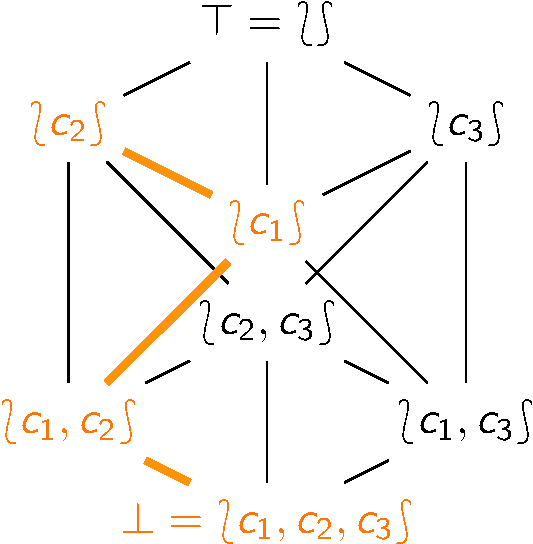
\includegraphics[width=2cm]{img/search-space.pdf} }; 
%  
\path[every node/.style={font=\sffamily\tiny}]
  (p2) edge (p1)
  (p3) edge (p1)
  ;
}
 
\onslide<5->{ 

\draw [isseorange] (5,0.7) -- (8,-1);
\node [isseorange] at (8.7,-0.5) {$\eta(c) = \lbag c \rbag$};
}

\onslide<6->{
\draw [issegrey] (5.7,-2) to [bend right] (4.2,-2);  
\node [issegrey] at (5,-1.5) {$(\SPDw{})^\#$};
}

\onslide<7->{
\draw [issegrey]  (4.2,-2.5) to [bend right] (5.7,-2.5);   
\node [issegrey] at (5,-3) {?};
}
\end{tikzpicture}
\end{center}

\end{frame}

\begin{frame}{Looking for freedom \ldots}
%\begin{itemize}
%\item (Konkrete) Kategorie $\mathsf{POSet}$: 
%\begin{itemize}
%\item[-] Objekte $\rightarrow$ partiell geordnete Mengen
%\item[-] Morphismen $\rightarrow$ monotone Funktionen
%\end{itemize}  
%\end{itemize}
\begin{lemma}[PVS-Freiheit \cite{knapp-schiendorfer2014}]
$\mathit{PVS}\langle P \rangle$ is the free partial valuation structure over the partial order $P$.
\end{lemma}


\begin{center}
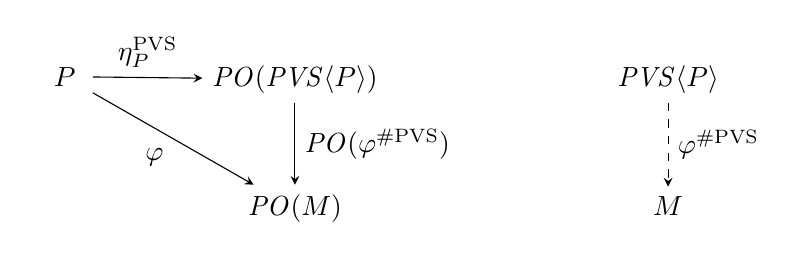
\begin{tikzpicture}
  \matrix (m) [matrix of math nodes,row sep=3em,column sep=4em,minimum width=2em,ampersand replacement=\&]
  {
     P \& \mathit{PO}(\mathit{PVS}\langle P \rangle) \& \& \mathit{PVS}\langle P \rangle \\
      \& \mathit{PO}(M) \& \& M \\};
  \path[-stealth]
    (m-1-1) edge node [above] {$\eta_P^{\mathrm{PVS}}$} (m-1-2)
            edge node [below left] {$\varphi$} (m-2-2)
    (m-1-2) edge node [right] {$\mathit{PO}( \varphi^{\# \mathrm{PVS} })$} (m-2-2)
    (m-1-4) edge [dashed] node [right] {$\varphi^{\# \mathrm{PVS} }$} (m-2-4)
;
\end{tikzpicture}
\end{center}

\cemph{Freie Konstruktionen}

\begin{itemize}
\item no junk
\item no confusion
\end{itemize}
\end{frame}

\begin{frame}[fragile]{In MiniBrass}
\begin{lstlisting}
type FreePVS = PVSType<mset[maxOccurrences] of 1..maxP> = 
  params { 
    array[int, 1..2] of 1..nScs: orderRelation;
    int: maxP;
    int: maxPerSc;
    int: maxOccurrences :: default('mbr.nScs * mbr.maxPerSc');
  } in 
  instantiates with "../mbr_types/free-pvs-type.mzn" {
    times -> multiset_union;
    is_worse -> isSmythWorse;
    top -> {};
  };
\end{lstlisting}

\begin{lstlisting}
PVS: fp = new FreePVS("fp") {
   soft-constraint c1: 'embed(x == 4, 3, 3)';
   soft-constraint c2: 'embed(x in {1,3,4}, 2, 3)';
   soft-constraint c3: 'embed(x <= 3, 1, 3)';
   
   orderRelation : '[| 2, 1 | 3, 1 |]';
   maxP: '3' ;
   maxPerSc : '2';
}; 

solve fp;
\end{lstlisting}
\end{frame}

\begin{frame}{Smyth in MiniBrass}
Die Smyth-Ordnung haben wir induktiv definiert: 
\begin{align*}
& p <_P q \Rightarrow T \mcup \lbag p \rbag \smyth{P} T \mcup \lbag q \rbag \\
& T \supmset U \Rightarrow T \smyth{P} U 
\end{align*}


Wie können wir sie nun für einen Constraint-Solver codieren?

\pause 

\begin{lemma}[Witness für $\smytheq{P}$ \cite{schiendorfer2017}] \label{lem:inj-upper}
$T \smytheq{P} U$ gilt genau dann wenn es eine injektive
Abbildung $h : S(U) \to S(T)$ (genannt \emph{Witness}-Funktion) mit $p \leq_P q$ wenn
$h(j, q) = (k, p)$ für alle $(j, q) \in S(U)$ gibt. 
\end{lemma}

\vspace*{3ex}
\begin{center}

\begin{tikzpicture}
\begin{scope}[node distance = 0.8cm] 
\node (lbrac) at (0,0) {$\lbag$};
\node [fill=CornflowerBlue!30,circle,draw,right of = lbrac] (a) {$1$}; 
\node [fill=CornflowerBlue!30,circle,draw,right of = a] (b) {$\RN{1}$};
\node [fill=CornflowerBlue!30,circle,draw,right of = b] (c) {$2$};
\node [right of = c] (rbrac)  {$\rbag$};
\end{scope}

\node  [right of = rbrac]  (smyth)  {$\smytheq{P}$};

\begin{scope}[node distance = 0.8cm] 

\node [right of = smyth](rlbrac) {$\lbag$};
\node [fill=ForestGreen!20,circle,draw,right of = rlbrac] (ra) {$2$}; 
\node [fill=ForestGreen!20,circle,draw,right of = ra] (rb) {$\RN{2}$};
\node [right of = rb] (rrbrac)  {$\rbag$};

\path (ra) edge[thick,isseorange,bend left,->] (a)
  (rb) edge[thick,isseorange,bend right,->] (b)
  ;
  
\end{scope}

\end{tikzpicture}
\end{center}

\end{frame}


\begin{frame}{Case Studies}
MiniBrass wird für verschiedene Anwendungen eingesetzt:

\vspace*{2ex}

\begin{itemize}
\item \alert<2->{Energiefallstudie}
\item \alert<2->{Studenten-Mentoren-Matching}
\item \alert<2->{Prüfungsterminfindung}
\item \alert<2->{Multi-User-Multi-Display}
\item Rekonfigurierbare Roboterteams
\item Potentiell: Rollenallokation im ODP
\end{itemize}
\end{frame}

\begin{frame}[fragile]{Mentor Matching}

\textbf{Ziel}: Teile Mentees (z.B. Studenten) Mentoren zu (z.B. Firmen), sodass
\begin{itemize}
\item Studenten sind sehr zufrieden mit ihren Mentoren
\item Firmen sind mit ihren Mentees ebenfalls zufrieden
\item Zweiseitige Präferenzen
\end{itemize}

\vspace*{2ex}

Zusätzliche Constraints sind vorhanden:

\begin{itemize}
\item[-] Jede Firme betreut zumindest $l$, höchstens aber $u$ Studenten
\item[-] Die Anzahl betreuter Studenten \emph{sollten} ungefähr gleich sein pro Firma (Fairness)
\item[-] Studenten, die eine Firma ``verachten'', sollen nicht gezwungen werden (\emph{harter Ausschluss} von Lösungen)
\end{itemize}
\end{frame}


\begin{frame}[fragile]{Studenten-Mentoren-Matching: Modell}
\begin{center}

\begin{tikzpicture}[>=stealth',shorten >=1pt,anchor=north west] 

%% FIRST OVERALL LAYER 

\draw[CornflowerBlue,thick,fill=white] (-0.4,0.7) rectangle (9,-6.7);
\node[CornflowerBlue] at (0, 0.6) {$\ltimes \quad \mathtt{lex}$};
\draw[CornflowerBlue,thick] (-0.4,-3.2) -- (9,-3.2);

% the logo

\begin{scope}
\node[pvsNode,minimum width=8.5cm,minimum height=3cm] (outer) at (0,0) {};


\begin{scope}[node distance=.6cm]

\draw [shading=axis,bottom color=black!10,top color=white,rounded corners] (0,0) -- (0,-1) -- (1.3,-1) -- (1.7,0) -- (0,0);
\draw(0,-1) -- ($ (outer.north east) + (0,-1) $);


% constraint relationship logo
\node[cpLogo] (upLogo) at (.55,-.2) {};
\node[cpLogo,below left of=upLogo] (leftLogo) {};
\node[cpLogo,below right of=upLogo] (rightLogo) {};  

\path[->]
  (leftLogo) edge node [right] {} (upLogo)
  (rightLogo) edge node [right] {} (upLogo)
;
\end{scope}

% spd parameter
\begin{scope}[node distance=0.7cm,xshift=3cm,scale=.5,transform shape]

% constraint relationship logo
\node[fill,circle,OliveGreen] (upLogo) at ($ (outer.north east) + (-1.3,-0.2) $) {};
\node[fill,circle,BrickRed,below of=upLogo] (centerLogo) {};
\node[fill,circle,gray,left of=centerLogo] (leftLogo) {};
\node[fill,circle,gray,right of=centerLogo] (rightLogo) {};  
\node[below of=centerLogo,yshift=.4em,font=\Large] {$\mathrm{SPD}$};
\path[->]
  (leftLogo) edge node [right] {} (upLogo)
  (centerLogo) edge node [right] {} (upLogo)
  (rightLogo) edge node [right] {} (upLogo)
;
\end{scope}

% EV
\begin{scope}[node distance=1.2cm]
\node[ anchor=center] at  ($ (outer.center) + (0.2,.9)$) {  $\mathtt{students}$ };


\node[main node, anchor=center,style={font=\sffamily\footnotesize}] (8) at ($ (outer.center) + (0,-0.2)$)   {$\mathtt{raubholzdelphi}$};

\node[main node, style={font=\sffamily\footnotesize},below right of=8,xshift=0.7cm] (4)  {$\mathtt{raubholzyouthlab}$};

\node[main node, style={font=\sffamily\footnotesize},below left of=8] (3) {$\mathtt{raubholzcupg}$};
\end{scope}
%\node[text width=2cm, anchor=west, left] at (4.3, 0.3) { CR };
%\node[text width=1cm, anchor=east, left] at (5.3, -2.3) { \textsc{SPD} };


\path[every node/.style={font=\sffamily\tiny},->]
  (3) edge node [right] {} (8)
  (4) edge node [right] {} (8)
;

\end{scope}


%% SECOND PVS 
%%%%%%%%%%%%%%%%%%%
\begin{scope}[yshift=-3.6cm]
\node[pvsNode,minimum width=8.5cm,minimum height=2.5cm] (outer) at (0,0) {};

% the logo

\begin{scope}[node distance=.6cm]

\draw [shading=axis,bottom color=black!10,top color=white,rounded corners] (0,0) -- (0,-1) -- (1.3,-1) -- (1.7,0) -- (0,0);
\draw(0,-1) -- ($ (outer.north east) + (0,-1) $);


% constraint relationship logo
\node[cpLogo] (upLogo) at (.55,-.2) {};
\node[cpLogo,below left of=upLogo] (leftLogo) {};
\node[cpLogo,below right of=upLogo] (rightLogo) {};  

\path[->]
  (leftLogo) edge node [right] {} (upLogo)
  (rightLogo) edge node [right] {} (upLogo)
;
\end{scope}

% spd parameter
\begin{scope}[node distance=.7cm,xshift=3cm,scale=.5,transform shape]

% constraint relationship logo
\node[fill,circle,OliveGreen] (upLogo) at ($ (outer.north east) + (-1.3,-0.2) $) {};
\node[fill,circle,BrickRed,below of=upLogo] (centerLogo) {};
\node[fill,circle,gray,left of=centerLogo] (leftLogo) {};
\node[fill,circle,gray,right of=centerLogo] (rightLogo) {};  
\node[below of=centerLogo,yshift=.4em,font=\Large] {$\mathrm{SPD}$};
\path[->]
  (leftLogo) edge node [right] {} (upLogo)
  (centerLogo) edge node [right] {} (upLogo)
  (rightLogo) edge node [right] {} (upLogo)
;

\end{scope}

% BIOGAS Plant 
\begin{scope}[node distance =0.8cm]
\node[main node, anchor=center, style={font=\sffamily\footnotesize}] (gf) at ($ (outer.center) + (0,0)$) {$\mathtt{delphirich}$};
\node[main node, style={font=\sffamily\footnotesize}] (ecs) [below  of=gf] {$\mathtt{delphikill}$};
\node[main node, style={font=\sffamily\footnotesize}] (ono) [right of=ecs,xshift=1.4cm] {$\mathtt{kasokyouth}$};
\end{scope}
%\node[main node, style={font=\sffamily\footnotesize},double] (hardConstraint) [below left of=7,xshift=-3.1,yshift=7] {$\mathsf{maxProd}$};
\node[ anchor=center] at  ($ (outer.center) + (0.2,.7)$) {  $\mathtt{companies}$ };


%\node[text width=2cm, anchor=west, left] at (4.3, 0.3) { CR };
%\node[text width=1cm, anchor=east, left] at (5.3, -2.3) { \textsc{SPD} };


\path[every node/.style={font=\sffamily\tiny},->]
  (ecs) edge node [right] {} (gf)
;

\end{scope}
\end{tikzpicture}
\end{center}
\end{frame}

\begin{frame}[fragile]{Studenten-Mentoren-Matching: Code}
\begin{lstlisting}
PVS: students = new ConstraintPreferences("students") {
   soft-constraint raubholzdelphi: 'worksAt[raubholz] = delphi';
   soft-constraint raubholzyouthlab: 'worksAt[raubholz] = youthlab';
   soft-constraint raubholzcupg: 'worksAt[raubholz] = cupgainini';
   
   crEdges : '[| mbr.raubholzyouthlab, mbr.raubholzdelphi | 
                 mbr.raubholzcupg, mbr.raubholzdelphi |]';
   useSPD: 'true' ;
}; 

PVS: companies = new ConstraintPreferences("companies") {
   soft-constraint delphi_kill: 'worksAt[kill] = delphi';
   soft-constraint delphi_rich: 'worksAt[rich] = delphi';
   soft-constraint kasokyouth: 'worksAt[kasok] = airtrain';
   
   crEdges : '[| mbr.delphi_kill, mbr.delphi_rich |]';
   useSPD: 'true' ;
}; 

solve students lex companies;
% solve companies lex students;
\end{lstlisting}
\end{frame}

\begin{frame}{Wann Constraint Preferences?}
\alert{Pro}:

\begin{itemize}
\item Wünschenswerte Bedingungen als boolesche Eigenschaften (``Constraints'')
\item Nicht alle erfüllbar
\item Nicht alle \textbf{vergleichbar}
\item \alert{Komparative} Bewertung möglich (``A ist mir wichtiger als B'')
\end{itemize}

\vspace*{2ex}
\hSecond{Contra}:

\begin{itemize}
\item Problem hat numerisches Ziel (Kosten, Verletzungen als Metrik)
\item Feingranulares Tuning für Gewichte von Constraints nötig
\item Ich will nur \emph{eine} Lösung am Ende.
\end{itemize}
\end{frame}

%% Weighted CSP and CFN 
\begin{frame}[fragile]{Prüfungstermine}

\textbf{Ziel}: Weise Prüfungstermine an Studenten zu, sodass
\begin{itemize}
\item Jeder Student stimmt seinem Termin zu 
\item Die Anzahl verschiedener Termine wird minimiert (um das Zeitinvestment der Dozenten zu schonen)
\end{itemize}

%\vspace*{2ex}
%\begin{parchment}
\begin{center}
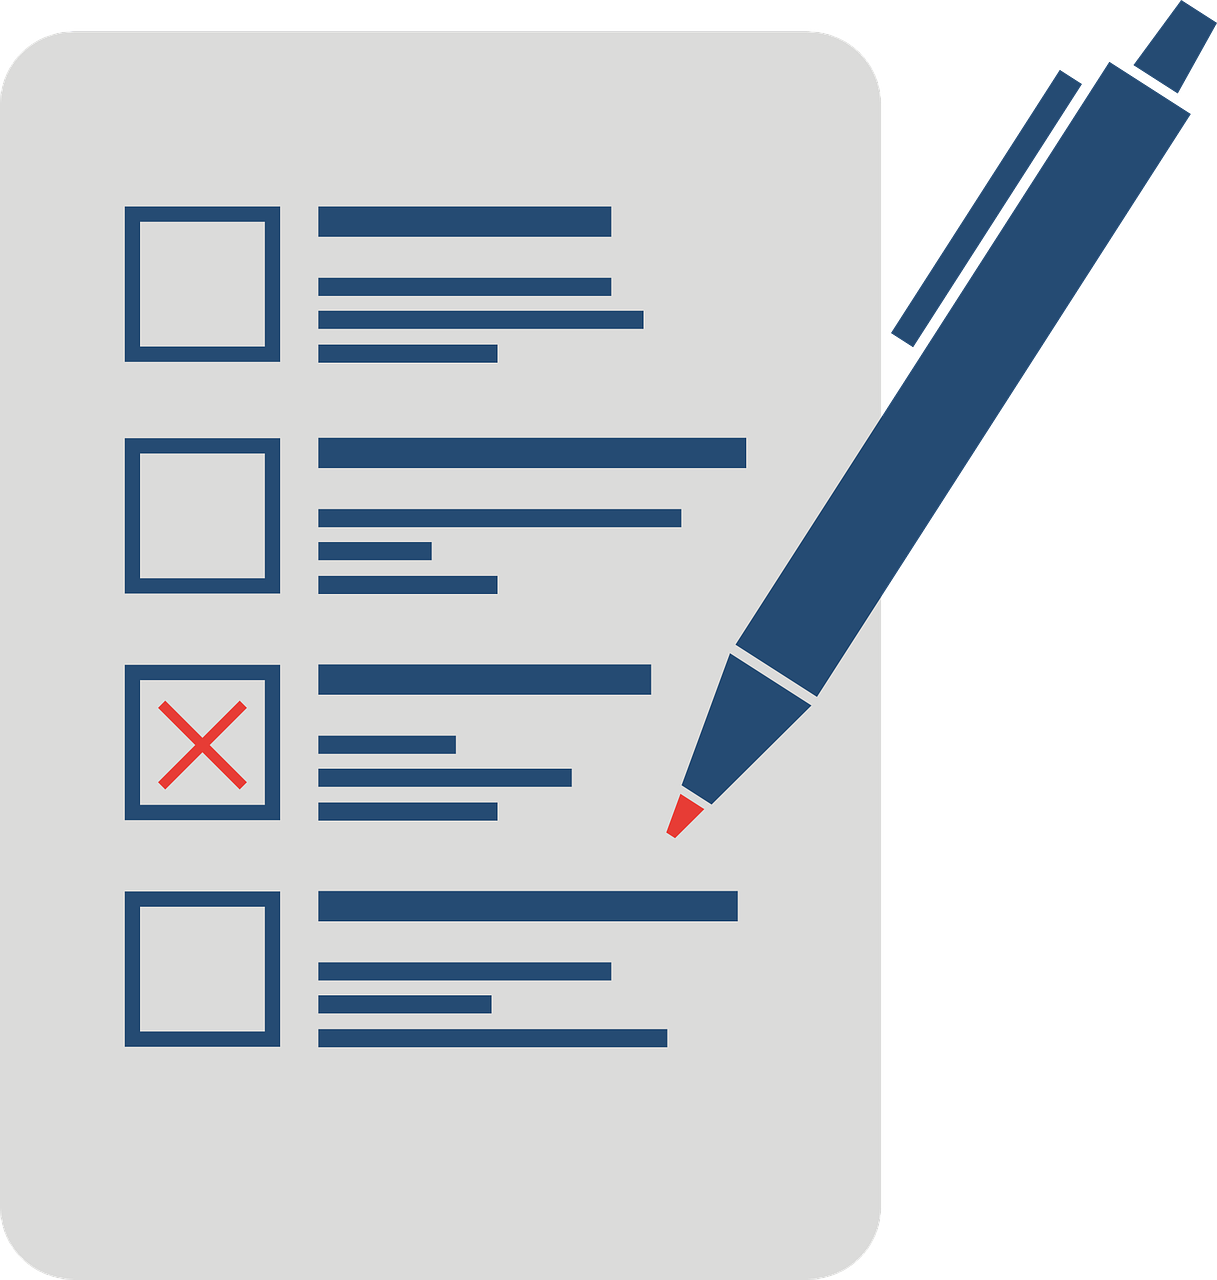
\includegraphics[width=.15\textwidth]{img/voting.png}
\hspace*{4ex}
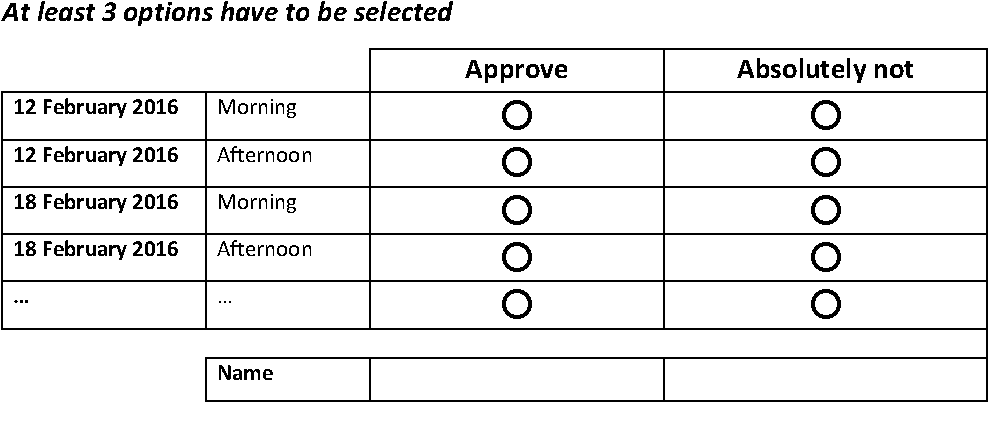
\includegraphics[width=.5\textwidth]{img/Voting.pdf}
\end{center}
%\end{parchment}

\begin{itemize}
\item Kein studentischer Wunsch sollte höher gewichtet werden
\item Prüfungsplan ist eine gemeinsame Entscheidung

\end{itemize}
\end{frame}

\begin{frame}[fragile]{Prüfungstermine: Modell}
\begin{center}
\begin{tikzpicture}[>=stealth',shorten >=1pt,anchor=north west] 

\draw[CornflowerBlue,thick,fill=white] (-0.4,0.7) rectangle (8,-6.7);
\node[CornflowerBlue] at (0, 0.6) {$\ltimes \quad \mathtt{lex}$};
\draw[CornflowerBlue,thick] (-0.4,-3.2) -- (8,-3.2);

\begin{scope}
\node[pvsNode,minimum width=7.5cm,minimum height=3cm] (outer) at (0,0) {};

% the logo

\begin{scope}[node distance=.6cm]

\draw [shading=axis,bottom color=black!10,top color=white,rounded corners] (0,0) -- (0,-1) -- (1.3,-1) -- (1.7,0) -- (0,0);
\draw(0,-1) -- ($ (outer.north east) + (0,-1) $);


% weighted constraints%s logo
\coordinate (beginLogo) at (0.4,0.0);
\node[cpLogo,anchor=south,scale=.8] (upLogo) at ($(beginLogo)+(0.3,-.45)$) {};

\draw [fill=black] ($(beginLogo)+(0,-.7)$) -- ($(beginLogo)+(0.1,-.4)$) -- ($(beginLogo)+(0.5,-.4)$) -- ($(beginLogo)+(0.6,-.7)$) -- ($(beginLogo)+(0,-.7)$);

\begin{scope}[scale=.6, transform shape]
\node[font=\Huge,anchor=east] at ($(outer.east) + (-1.1,1.8)$) {$100$};
\node[font=\Large,anchor=east] at ($(outer.east) + (-1.1,1.2)$) {$\mathrm{maxWeight}$};
\end{scope}
\end{scope}

\node[ anchor=center] at  ($ (outer.center) + (0.2,.7)$) {  $\mathtt{students}$ };

\node[weightNode,text=white,anchor=west,text width=1.5cm,text height=.17cm,align=right] (bg) at ($ (outer.center) + (-2,0.1)$)   {\hfill 1};
\node[main node,draw,anchor=west] (limitBu) at ($ (outer.center) + (-2,0.1)$)   {$\mathtt{meerfluss}$};

\node[weightNode,text=white,anchor=west,text width=1.3cm,text height=.17cm,align=right] (bg2) at ($(limitBu.west)+(0,-.5)$)   {\hfill 1};
\node[main node, anchor=west, style={font=\sffamily\footnotesize}] (earlyBird) at ($(limitBu.west)+(0,-.5)$)  {$\mathtt{ayman}$};

\node[weightNode,text=white,anchor=west,text width=1.3cm,text height=.19cm,align=right] (bg3) at ($(earlyBird.west)+(0,-.5)$)   {\hfill 1};
\node[main node, anchor=west, style={font=\sffamily\footnotesize}] (prefBatteryLevel) at ($(earlyBird.west)+(0,-.5)$)  {$\mathtt{kanye}$};

\node[weightNode,text=white,anchor=west,text width=1.4cm,text height=.17cm,align=right] (bg) at ($ (outer.center) + (1,0.1)$)   {\hfill 1};
\node[main node,draw,anchor=west] (limitBu) at ($ (outer.center) + (1,0.1)$)   {$\mathtt{raubholz}$};

\node[weightNode,text=white,anchor=west,text width=1.7cm,text height=.17cm,align=right] (bg2) at ($(limitBu.west)+(0,-.5)$)   {\hfill 1};
\node[main node, anchor=west, style={font=\sffamily\footnotesize}] (earlyBird) at ($(limitBu.west)+(0,-.5)$)  {$\mathtt{schraubale}$};

\node[weightNode,text=white,anchor=west,text width=2.3cm,text height=.19cm,align=right] (bg3) at ($(earlyBird.west)+(0,-.5)$)   {\hfill 101};
\node[main node, anchor=west, style={font=\sffamily\footnotesize}] (prefBatteryLevel) at ($(earlyBird.west)+(0,-.5)$)  {$\mathtt{kanye-urlaub}$};


\end{scope}

%% SECOND PVS 
%%%%%%%%%%%%%%%%%%%
\begin{scope}[yshift=-3.6cm]
\node[pvsNode,minimum width=7.5cm,minimum height=2.5cm] (outer) at (0,0) {};

% the logo

\begin{scope}[node distance=.6cm]

\draw [shading=axis,bottom color=black!10,top color=white,rounded corners] (0,0) -- (0,-1) -- (1.3,-1) -- (1.7,0) -- (0,0);
\draw(0,-1) -- ($ (outer.north east) + (0,-1) $);


\node at (.1,-.3) {\Huge \EUR};
\node at (.6,-0.1) {\Large $\mathbb{Z}$};


\end{scope}

% spd parameter
\begin{scope}[node distance=.7cm,xshift=3cm,scale=.5,transform shape]

% cfn logos
\draw[thick,->] ($(outer.east) + (-1.3,2)$) -- ($(outer.east) + (-1.3,1)$);
\node[font=\Large,anchor=east] at ($(outer.east) + (-0.5,0.9)$) {$\mathrm{Minimize}$};


\node[font=\Huge,anchor=east] at ($(outer.east) + (-2.7,1.5)$) {$\mathrm{\sum}$};
\node[font=\Large,anchor=east] at ($(outer.east) + (-2.7,0.9)$) {$\mathrm{Sum}$};

\end{scope}

% BIOGAS Plant 
\begin{scope}[node distance =0.8cm]
\node[main node, anchor=center, style={font=\sffamily\footnotesize}] (gf) at ($ (outer.center) + (0,-.5)$) {$\mathtt{scheduledDates}$};
\end{scope}
%\node[main node, style={font=\sffamily\footnotesize},double] (hardConstraint) [below left of=7,xshift=-3.1,yshift=7] {$\mathsf{maxProd}$};
\node[ anchor=center] at  ($ (outer.center) + (0.2,.7)$) {  $\mathtt{teachers}$ };
\end{scope}
\end{tikzpicture}
\end{center}

\end{frame}

\begin{frame}[fragile]{Prüfungstermine: Code}

\begin{lstlisting}
PVS: students = new WeightedCsp("students") {
   maxWeight: '100';
   soft-constraint raubholz:   'sd[raubholz] in {monday, tuesday}';   
   soft-constraint schraubale: 'sd[schraubale] in {tuesday, wednesday}';
   soft-constraint meerfluss:  'sd[meerfluss] in {tuesday}';
   soft-constraint ayman:   'sd[ayman] in {monday, tuesday}';
   soft-constraint kanye:     'sd[kanye] in {monday, wednesday}';
   % hard by weight (less than bottom)
   soft-constraint kanye-urlaub: 'sd[kanye] != tuesday'
                                :: weights('101'); 
}; 
PVS: teachers = new CostFunctionNetwork("teachers") {
   soft-constraint scheduledDates: 'scheduledDates';
}; 
solve students lex teachers;
\end{lstlisting}

\begin{Verbatim}[fontsize=\small]
Scheduled: [1, 2, 2, 1, 1], Distinct dates: 2
Valuations: mbr_overall_students = 0; mbr_overall_teachers = 2
\end{Verbatim}
\end{frame}

\begin{frame}{Wann Weighted CSP / Cost Function Networks?}
\alert{Pro}:

\begin{itemize}
\item Feintuning von Gewichten für Soft Constraints (evt. erlernt vom Benutzer)
\item Skalare Kostenfunktion ist offensichtlich (Produktionskosten, Spanne der Task-Zuweisung) 
\item Fehler können per Distanz angegeben und minimiert werden (50 KW Abweichung ist schlimmer als 10 KW Abweichung)
\item Lösungszeit ist kritisch -- keine Auswahlmöglichkeiten nötig
\end{itemize}

\vspace*{2ex}
\hSecond{Contra}:

\begin{itemize}
\item Es gibt tatsächlich unvergleichbare Kriterien.
\item Ich will mir für eine Ordnung keine Gewichtung ``ausdenken'' müssen -- besonders wenn sich Soft Constraints häufig ändern.
\item Viele Entscheidungsvarianten gewünscht (nicht nur ``skalares Optimum'') -- z.B. in Offline-Entscheidungssituationen
\end{itemize}
\end{frame}

\begin{frame}[fragile]{Probabilistic Constraints \cite{fargier1993uncertainty}}
\begin{figure}[t]
\centering
\begin{tikzpicture}[>=stealth',shorten >=1pt,anchor=north west] 


\begin{scope}
\node[pvsNode,minimum width=4cm,minimum height=3cm] (outer) at (0,0) {};

% the logo

\begin{scope}[node distance=.6cm]

\draw [shading=axis,bottom color=black!10,top color=white,rounded corners] (0,0) -- (0,-1) -- (1.3,-1) -- (1.7,0) -- (0,0);
\draw(0,-1) -- ($ (outer.north east) + (0,-1) $);

% probabilistic constraints%s logo

\node at (1,-0.1) {\Large $\mathbb{P}$};
\draw(0.7,-0.3) -- (0.7,-.9);
\draw(0.3,-0.7) -- (1.1,-.7);

\draw [thick] plot [smooth, tension=.6] coordinates {(0.3,-0.59) (0.55,-0.59) (0.7,-0.39)  (0.85,-0.59) (1.1,-0.59) };

\end{scope}

\node[main node,draw,anchor=west] (limitBu) at ($ (outer.center) + (-1,0.1)$)   {\texttt{beerSupp}};

\node[main node, anchor=west, style={font=\sffamily\footnotesize}] (prefBatteryLevel) at ($(limitBu.west)+(1.2,-.6)$)  {\texttt{beerDem}};


\end{scope}

\end{tikzpicture}
\end{figure}
\begin{lstlisting}
type ProbabilisticConstraints = PVSType<bool, 0.0 .. 1.0> = 
  params {
    array[1..nScs] of float: probs :: default('1.0');
  } in  
  instantiates with "soft_constraints/mbr_types/probabilistic_type.mzn" {
    times -> prod;
    is_worse -> is_worse_prob;
    top -> 1.0;
};   
[...]
soft-constraint beerDem: 'dem1 + dem2 >= 10' :: probs('0.7');
soft-constraint beerSupp: 'sup1 + sup2 <= 10' :: probs('0.2');
\end{lstlisting}
\end{frame}

\begin{frame}{Wann Probabilistic Constraints?}
\alert{Pro}:

\begin{itemize}
\item Wenn ich unsicher bin, ob ein Constraint wirklich vorhanden sein wird.
\item Wenn ich die Wahrscheinlichkeit wissen will, dass \emph{alle} (vl. noch nicht sicheren) Constraints erfüllt sind
\item Weighted Variante straightforward
\end{itemize}

\vspace*{2ex}
\hSecond{Contra}:

\begin{itemize}
\item Andere Verteilungen außer ``Münzwurf'' nicht behandelt (Constraint gilt oder nicht)
\item Bildet keine Szenarien ab
\item Eignet sich nicht für einen erwarteten Kostenwert
\end{itemize}
\end{frame}

\begin{frame}[fragile]{Fuzzy Constraints \cite{ruttkay1994fuzzy}}
\begin{figure}[t]
\centering
\begin{tikzpicture}[>=stealth',shorten >=1pt,anchor=north west] 


\begin{scope}
\node[pvsNode,minimum width=4cm,minimum height=3cm] (outer) at (0,0) {};

% the logo

\begin{scope}[node distance=.6cm]

\draw [shading=axis,bottom color=black!10,top color=white,rounded corners] (0,0) -- (0,-1) -- (1.3,-1) -- (1.7,0) -- (0,0);
\draw(0,-1) -- ($ (outer.north east) + (0,-1) $);

\node at (1,-0.1) {\Large $\mathrm{\mu}$};


\draw(0.4,-0.1) -- (0.4,-.8);
\draw(0.3,-0.7) -- (1.2,-.7);
\node[scale=0.5,transform shape,anchor=east] at (0.35,-0.6) {0};
\node[scale=0.5,transform shape,anchor=east] at (0.35,-0.25) {1};

\draw [thick] plot [smooth, tension=.2] coordinates { (0.4,-0.59) (0.6,-0.59) (0.85,-0.25)(1.05,-0.25)};

\end{scope}

\begin{scope}[node distance=.7cm,xshift=1.7cm,scale=.5,transform shape]

%\node[font=\Huge] at (2.7,-0.3) {$\mathrm{\Min}$};
%\node[font=\Large] at (2.6,-1.3) {$\mathrm{Minimum}$};

\end{scope}
\node[main node,draw,anchor=west] (limitBu) at ($ (outer.center) + (-1,0.1)$)   {\texttt{taste1}};

\node[main node, anchor=west, style={font=\sffamily\footnotesize}] (earlyBird) at ($(limitBu.west)+(1,-.8)$)  {\texttt{taste2}};



\end{scope}

\end{tikzpicture}
\end{figure}

\begin{lstlisting}
type FuzzyConstraints = PVSType<0.0 .. 1.0> = 
  instantiates with "soft_constraints/mbr_types/fuzzy_type.mzn" {
    times -> min;
    is_worse -> is_worse_fuzzy;
    top -> 1.0;
};
PVS: fz1 = new FuzzyConstraints("fz1") {
   soft-constraint taste1: 'fbinary_fuzzy([1.0, 0.8, 0.3, 0.7], main, wine)';
   soft-constraint taste2: 'fbinary_fuzzy([1.0, 0.8, 0.8, 1.0], main, dessert)';
}; 
solve fz1;
\end{lstlisting}
\end{frame}

\begin{frame}{Wann Fuzzy Constraints?}
\alert{Pro}:

\begin{itemize}
\item Wenn ich Kombinationen (z.B. Essen+Wein) als Zufriedenheitsprozentsatz ausdrücken will.
\item Wenn Soft Constraints relativ formuliert werden kann (als Verhältnis), z.B. \texttt{supply / Demand}  
\item Einfach zu interpretierender, einzelner Erfüllungsgradwert (0.7 bedeutet, der \emph{schlechteste} Soft Constraint bildet  auf 0.7 ab)
\end{itemize}

\vspace*{2ex}
\hSecond{Contra}:

\begin{itemize}
\item Sehr strenge Semantik bei Abbildung auf geringsten Wert 
\item Floating Point Unterstützung in Constraint Solvern dürftig (daher besser nach Weighted CSP mit Morphismus abbilden)
\end{itemize}
\end{frame}
%
\begin{frame}[fragile]{MiniBrass}

\begin{center}

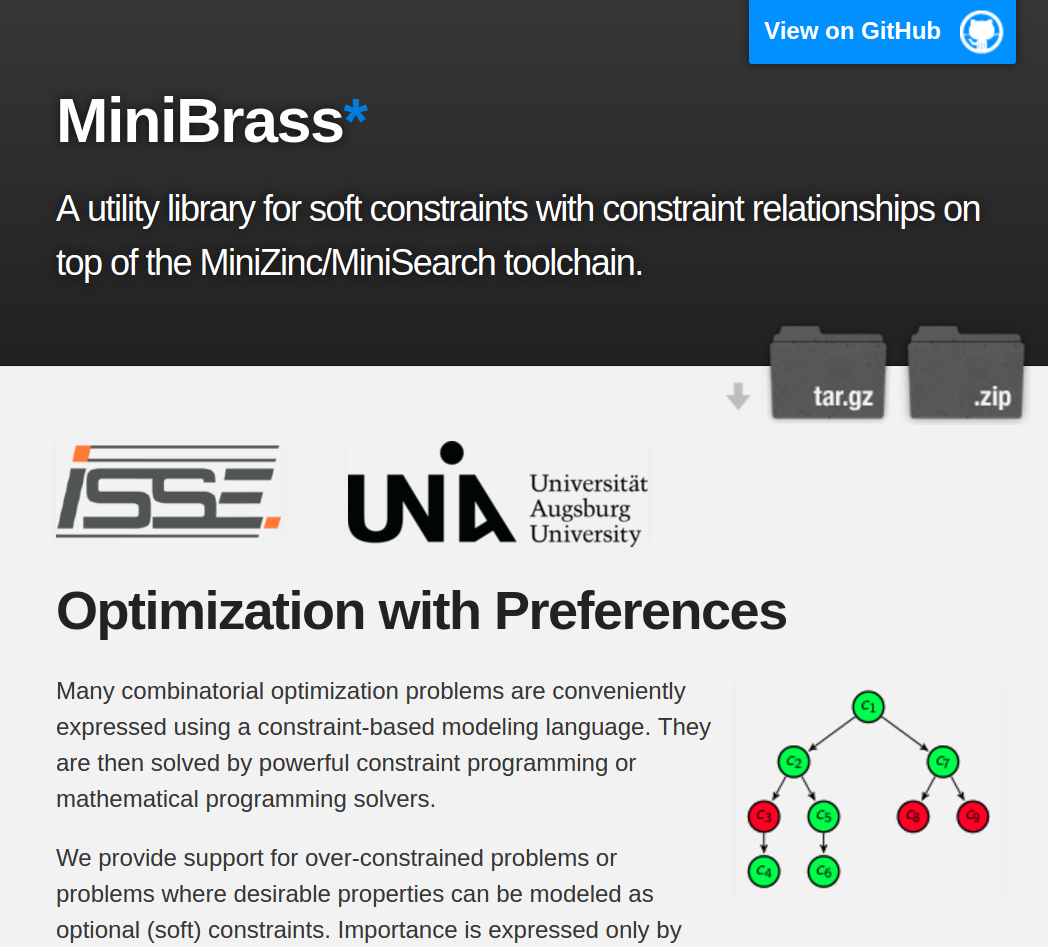
\includegraphics[width=.5\textwidth]{img/minibrass.png}

\vspace*{2ex}

\url{http://isse-augsburg.github.io/minibrass/}

\end{center}

\end{frame}

\begin{frame}[fragile]{MiniBrass: HelloWorld}
\begin{columns}[onlytextwidth,T]
    
    \begin{column}{.40\textwidth}
          
    \hSecond{Basismodell (MiniZinc)}
    \begin{lstlisting}
include "hello_o.mzn"; 
include "soft_constraints/
   pvs_gen_search.mzn"; 
% the basic, "classic" CSP 
set of int: DOM = 1..3;

var DOM: x; var DOM: y; 
var DOM: z;
% add. *hard* constraints
% e.g. constraint x < y;

solve search pvs_BAB();
\end{lstlisting}
    \end{column}
    
    \begin{column}{.55\textwidth}
  	\hFirst{Präferenzmodell (MiniBrass)} 
  	\begin{lstlisting}
PVS: cr1 = 
  new ConstraintRelationships("cr1") {
   soft-constraint c1: 'x + 1 = y';
   soft-constraint c2: 'z = y + 2';
   soft-constraint c3: 'x + y <= 3';
   
   crEdges : '[| mbr.c2, mbr.c1 | 
                  mbr.c3, mbr.c1 |]';
   useSPD: 'true' ;
}; 

solve cr1;
\end{lstlisting}

    \end{column}
  \end{columns}
  \pause
  \begin{verbatim}
Solution:  x = 1; y = 2; z = 1
Valuations:  mbr_overall_cr1 = {c2}
----------
==========
  \end{verbatim}
  \begin{textblock*}{3cm}[1,1](\textwidth+0.5cm,\textheight-0.3cm)
%\textblockcolour{issegrey!20}
\begin{center}
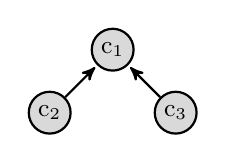
\begin{tikzpicture}[auto,
                    ->,>=stealth',shorten >=1pt,thick,
                    node distance=.7cm,inner sep=2pt,
                    constraint/.style={circle,fill=black!15,draw,font=\sffamily\small}]
\node[constraint node] (1) at (0, 0)                   {$\mathrm{c}_1$};
\node[constraint node] (2) at ($ (1) + (-0.8, -0.8) $) {$\mathrm{c}_2$};  
\node[constraint node] (3) at ($ (1) + ( 0.8, -0.8) $) {$\mathrm{c}_3$};  
%  
\path[every node/.style={font=\sffamily\tiny}]
  (2) edge (1)
  (3) edge (1)
  ;
  

\end{tikzpicture}
\end{center}
\end{textblock*}
\end{frame}


\begin{frame} \small
\frametitle{Single-Predecessor-Dominance (SPD) Lifting}

\cemph{isWorseThan}-Relation für Mengen verletzter Constraints~\cite{Schiendorfer13}
%
\bgroup\abovedisplayskip=4pt\belowdisplayskip=12pt
\begin{gather*}
  V \uplus \{ c \}  \supset_{\mathsf{SPD}}  V 
\\
  V \uplus \{ c_{\mathrm{gold}} \}  \supset_{\mathsf{SPD}}  V \uplus \{ c_{\mathrm{silber}} \}
\quad\text{wenn $c_{\mathrm{silber}}$ weniger wichtig als $c_{\mathrm{gold}}$}
\end{gather*}
\egroup

\begin{center}
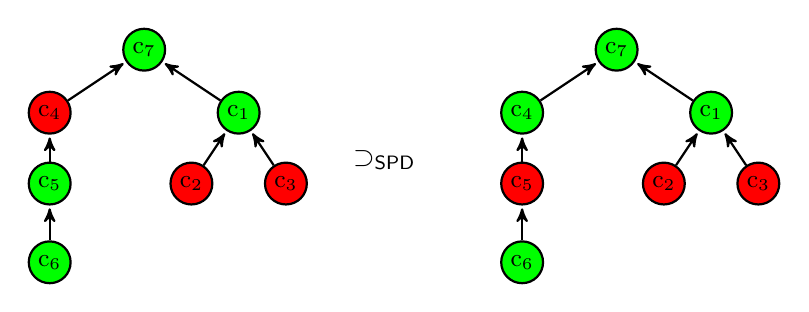
\begin{tikzpicture}[auto,
                    ->,>=stealth',shorten >=1pt,thick,
                    node distance=1cm,inner sep=2pt,
                    constraint/.style={circle,fill=black!15,draw,font=\sffamily\small}]
\begin{scope}
\node[constraint,fill=green] (1) at (0, 0)                   {$\mathrm{c}_7$};
\node[constraint,fill=red] (2) at ($ (1) + (-1.2, -0.8) $) {$\mathrm{c}_4$};  
\node[constraint,fill=green]   (3) at ($ (2) + (0.0, -0.9) $) {$\mathrm{c}_5$};  
\node[constraint,fill=green] (4) at ($ (3) + ( 0.0, -1.0) $) {$\mathrm{c}_6$};
\node[constraint,fill=green] (7) at ($ (1) + ( 1.2, -0.8) $) {$\mathrm{c}_1$};  
\node[constraint,fill=red]   (8) at ($ (7) + (-0.6, -0.9) $) {$\mathrm{c}_2$};  
\node[constraint,fill=red]   (9) at ($ (7) + ( 0.6, -0.9) $) {$\mathrm{c}_3$};  
%  
\path[every node/.style={font=\sffamily\tiny}]
  (2) edge (1)
  (7) edge (1)
  (3) edge (2)
  (4) edge (3)
  (8) edge (7)
  (9) edge (7)
  ;
\end{scope}
%
\begin{scope}[xshift=6cm]
\node[constraint,fill=green] (1) at (0, 0)                   {$\mathrm{c}_7$};
\node[constraint,fill=green]   (2) at ($ (1) + (-1.2, -0.8) $) {$\mathrm{c}_4$};  
\node[constraint,fill=red] (3) at ($ (2) + (0.0, -0.9) $) {$\mathrm{c}_5$};  
\node[constraint,fill=green] (4) at ($ (3) + ( 0.0, -1.0) $) {$\mathrm{c}_6$};  
\node[constraint,fill=green] (7) at ($ (1) + ( 1.2, -0.8) $) {$\mathrm{c}_1$};  
\node[constraint,fill=red]   (8) at ($ (7) + (-0.6, -0.9) $) {$\mathrm{c}_2$};  
\node[constraint,fill=red]   (9) at ($ (7) + ( 0.6, -0.9) $) {$\mathrm{c}_3$};  
%  
\path[every node/.style={font=\sffamily\tiny}]
  (2) edge (1)
  (7) edge (1)
  (3) edge (2)
  (4) edge (3)
  (8) edge (7)
  (9) edge (7)
  ;
\end{scope}
%
\node (R) at (3.05, -1.4) {$ \supset_{\mathsf{SPD}}$};
\end{tikzpicture}
\end{center}

\begin{itemize}
\item Bekannt als \emph{Smyth-Ordnung} (Powerdomains) \hfill \cite[Ch.~9]{amadio-curien:1998}
\item Entsteht aus \emph{freier Konstruktion} über Constraint-Relationship.\hfill \cite{knapp-schiendorfer2014ictai}
\end{itemize}

%
%\cemph{Ordnungs}relation über Zuweisungen 
%\bgroup\abovedisplayskip4pt
%\begin{equation*}
%  w \SPDord{R} v \iff \{ c \in C \mid v \not\models c \} \mathrel{({\SPDrel{R}})^{+}} \{ c \in C \mid w \not\models c \}
%\end{equation*}
%\egroup

\end{frame}

\tikzset{onslide/.code args={<#1>#2}{%
  \only<#1>{\pgfkeysalso{#2}}
}}
\tikzstyle{highlight}=[isseorange,ultra thick]
\tikzstyle{highlight2}=[CornflowerBlue,ultra thick]
\begin{frame}[fragile]{Constraint-Optimierung mit PVS}
Der partiell geordnete Bewertungsraum



\begin{figure}[!t]
\begin{center}
\begin{tikzpicture}[scale=0.77,auto]

% single PVS
\node (bot) at (0,0) {\alert{$\bot = \{c_1, c_2, c_3 \}$}};
\node (c1c2) at (-2,1) {\alert<2->{$\{c_1, c_2\}$}};
\node (c2c3) at (0,2) {$\{c_2, c_3\}$};
\node (c1c3) at (2,1) {$\{c_1, c_3\}$};

\node (c1) at (0,3) {\alert<3->{$\{c_1\}$}};
\node (c2) at (-2,4) {\alert<4->{$\{c_2\}$}};
\node (c3) at (2,4) {$\{c_3\}$};
%\node (a) at (-1,0.5) {$a$};
%\node (b) at (-1,1.5) {$b$};
%\node (c) at (1,1) {$c$};
\node (top) at (0,5) {$\top = \emptyset$};

\node[text width=2cm] (verb) at (4,0) {     };
\path[-]
(bot) edge[onslide={<2->{highlight}}] (c1c2)
      edge (c2c3)
      edge (c1c3)
(c1c2) edge (c2c3)
(c1c3) edge (c2c3)
(c1c3) edge (c1)
(c1c3) edge (c3)
(c2c3) edge (c2)
(c2c3) edge (c3)
(c1c2) edge[onslide={<3->{highlight}}] (c1)
(c1c2) edge (c2)
(c1) edge[onslide={<4->{highlight}}] (c2)
(c1) edge (c3)
(c2) edge (top)
(c1) edge (top)
(c3) edge (top)
      ;
%(a) edge (b)
%(b) edge (top)
%(bot) edge (c)
%(c) edge (top)
;

\end{tikzpicture}
\end{center}
\label{fig:nosuprema}
\end{figure}
\begin{lstlisting}
function ann: pvs_BAB() =
       repeat(
           if next() then 
                 print("Intermediate solution:") /\ print() /\
                 commit() /\ postGetBetter()
           else break endif       );
\end{lstlisting}
\begin{textblock*}{2.5cm}[1,1](\textwidth-8.8cm,\textheight-4.03cm)
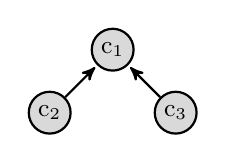
\begin{tikzpicture}[auto,
                    ->,>=stealth',shorten >=1pt,thick,
                    node distance=.7cm,inner sep=2pt,
                    constraint/.style={circle,fill=black!15,draw,font=\sffamily\small}]
\node[constraint node] (1) at (0, 0)                   {$\mathrm{c}_1$};
\node[constraint node] (2) at ($ (1) + (-0.8, -0.8) $) {$\mathrm{c}_2$};  
\node[constraint node] (3) at ($ (1) + ( 0.8, -0.8) $) {$\mathrm{c}_3$};  
%  
\path[every node/.style={font=\sffamily\tiny}]
  (2) edge (1)
  (3) edge (1)
  ;
  

\end{tikzpicture}
\begin{Verbatim}[fontsize=\small]
c1: 'x + 1 = y';
c2: 'z = y + 2';
c3: 'x + y <= 3';   
\end{Verbatim}
\end{textblock*}

\begin{textblock*}{4cm}[1,1](\textwidth+0.5cm,\textheight-3.03cm)

\onslide<2->{

{ \tt  \small
x = 1; y = 1; z = 1 \newline
Valuation = \{c1,c2\}
}
}

\onslide<3->{
{ \tt  \small
----------

x = 1; y = 1; z = 3 \newline
Valuation = \{c1\}
}
}


\onslide<4->{
{ \tt  \small
----------

x = 1; y = 2; z = 1 \newline
Valuations = \{c2\}

----------

==========

}
}
\end{textblock*}
\end{frame}

\tikzset{
    process/.style={rectangle,rounded corners,draw=black, top color=isseorange!5, bottom color=isseorange!30},
    file/.style={rectangle,draw=black}
}
\begin{frame}{MiniBrass: Workflow} \small

\vspace*{-2ex}
\alert{Architektur}

\begin{center}
\vspace*{-10ex}
\begin{tikzpicture}[>=stealth,auto,every node/.style={
anchor=base,
text depth=.5ex,
text height=2ex,
minimum height=2ex,
align=center,
circle,
minimum width=1em}]
\matrix (magic) [nodes in empty cells, ampersand replacement=\&,row sep=0.5cm,column sep=0.5cm]
{
\node{}; \&\node[draw, file,isseorange,thick](mbrlibs){\texttt{mbrlibs.mzn}}; \& \& \node[draw, file,isseorange,thick](types){\texttt{types.mbr}}; \\
\node {};\& \node[draw, file,CornflowerBlue,thick](mbr){\texttt{prefs.mbr}};   \& \& \node[draw, isseorange,thick,process](mbr2mzn){\texttt{mbr2mzn}}; \\
\node {};\& \& \& \node[draw, file,isseorange,thick](compiledMzn){\emph{prefs\_o.mzn}}; \\
%    \&  \&  \node(inv){}; \&  \\
\node {};\& \node[draw, file,CornflowerBlue!80](f1){\texttt{model.mzn}}; \& \& \node[draw, process](mzn2fzn){\texttt{mzn2fzn}}; \& \& \node[draw, file](output){\emph{output}};  \\
%    \&  \&  \node(inv){}; \&  \\
\node {};\& \node[draw, file,CornflowerBlue!80](mod){\texttt{data.dzn}}; \& \&  \\
\node {};\& \node[draw, file](mznlibs){\texttt{mznlibs.mzn}};\& \& \node[draw, file](fzn){\texttt{compiled.fzn}}; \& \& \node[draw, process](solve){\texttt{solve}};  \\
\node {};\& \& \\
};

\draw[dashed,->] (f1) -- (mzn2fzn);
\draw[dashed,->] (mbr) -- (mbr2mzn);
\draw[dashed,->] (mod) -- (mzn2fzn);
\draw[dashed,-] (types) -- (mbrlibs);
\draw[dashed,-] (types) -- (mbr);
%\draw[dashed,->] (mbrlibs) -- (mzn2fzn);
%\draw[dashed] (mbrlibs) -- (mbr);
\draw[dashed,->] (compiledMzn) -- (mzn2fzn);
\draw[dashed,->] (mznlibs) -- (mzn2fzn);
\draw[dashed,->] (fzn) -- (solve);
\draw[->] (mbr2mzn) -- (compiledMzn);

\draw[->] (mzn2fzn) -- (fzn);
\draw[->] (solve) -- (output);
%\draw[dashed] (globals) -- (inv);

%\onslide<4->{  
%\node[overlay,align=left,rectangle callout,%
%      callout absolute pointer=(mbrlibs.west),fill=CornflowerBlue!50] at (-4.5,5) {PVS-Prädikate};}

\onslide<4->{  
\node[overlay,align=left,rectangle callout,%
      callout absolute pointer=(mbrlibs.north),fill=isseorange!50] at (-3,7.5) {Implementierte Funktionen und Prädikate};}
            
\onslide<3->{  
\node[overlay,align=left,rectangle callout,%
      callout absolute pointer=(types.north),fill=isseorange!50] at (2,7.5) {PVS-Typdefinitionen};} 
     
\onslide<3->{  
\node[overlay,align=left,rectangle callout,%
      callout absolute pointer=(mbr.west),fill=CornflowerBlue!50] at (-3.7,4.5) {PVS-Instanzen, Kombinationen};} 
     
\end{tikzpicture}
\end{center}
\vspace*{-25ex}

\end{frame}


\begin{frame}[fragile]{PVS-Typdefinitionen}
\begin{lstlisting}
type ConstraintRelationships = PVSType<bool, set of 1..nScs> = 
  params { 
    array[int, 1..2] of 1..nScs: crEdges; % adjacency matrix
    bool: useSPD;
  } in 
  instantiates with "../mbr_types/cr_type.mzn" {
    times -> link_invert_booleans;
    is_worse -> is_worse_cr;
    top -> {};
  };
\end{lstlisting}
\begin{itemize}
\item \texttt{PVSType<S,E>} Unterscheidet zur einfacheren Verwendung zwischen 
\begin{itemize}
\item[] Spezifikationstyp $S$ 
\item[] Elementtyp $E$
\end{itemize} 
\item Kombinationsoperation: $\mathtt{times} : S^n \to E$
\item Ordnungsrelation: $\mathtt{isWorse} \subseteq E \times E$
\end{itemize}
\end{frame}

%\begin{frame}[fragile]{PVS-Definitionen}
%Innerhalb von \texttt{../mbr\_types/cr\_type.mzn}:
%\begin{lstlisting}
%function var set of int: 
%  link_invert_booleans(array[int] of var bool: b...
%
%% gives us access to constraint relationship predicates 
%include "soft_constraints/spd_worse.mzn";
%include "soft_constraints/tpd_worse.mzn";
%
%predicate is_worse_cr(var set of int: violated1, 
%                      var set of int: violated2,
%                      par int: nScs, array[int, 1..2] of par int: crEdges, 
%                      par bool: useSPD) =
%let {  par set of int: softConstraints = 1..nScs; } in (                    
%    if useSPD then
%      spd_worse(violated1, violated2, softConstraints, crEdges)
%    else
%      tpd_worse(violated1, violated2, softConstraints, crEdges)
%    endif);
%
%\end{lstlisting}
%\end{frame}

\begin{frame}[fragile]{PVS-Instanziierung (Revisited)}
\begin{lstlisting}
PVS: cr1 = new ConstraintRelationships("cr1") {
   soft-constraint c1: 'x + 1 = y';
   soft-constraint c2: 'z = y + 2';
   soft-constraint c3: 'x + y <= 3';
   
   crEdges : '[| mbr.c2, mbr.c1 | mbr.c3, mbr.c1 |]';
   useSPD: 'false' ;
}; 
\end{lstlisting}
\begin{itemize}
\item Jeder Soft-Constraint ein $S$-Ausdruck (hier z.B. $\mathtt{bool}$)
\item Mittels der Funktion $\mathtt{times}$ auf einen $E$-Wert abgebildet
\item Ausdrücke in einfachen Anführungszeichen: \alert{MiniZinc}-Code (nicht geparst, bis auf \texttt{mbr.}-Präfixe)
\item Parameter aus \texttt{PVSType} müssen Wert erhalten
\end{itemize}
\end{frame}

\begin{frame}[fragile]{Weitere PVS-Typen}
\begin{lstlisting}
type WeightedCsp = PVSType<bool, int> = 
  params {
    int: k; 
    array[1..nScs] of 1..k: weights :: default('1');
  } in  
  instantiates with "../mbr_types/weighted_type.mzn" {
    times -> weighted_sum;
    is_worse -> is_worse_weighted;
    top -> 0;
  };
  
type CostFunctionNetwork = PVSType<0..k> = 
  params {
    int: k :: default('1000'); 
  } in  instantiates with "../mbr_types/cfn_type.mzn" {
    times -> sum;
    is_worse -> is_worse_weighted; 
    top -> 0;
 };
\end{lstlisting}
\end{frame}

\begin{frame}[fragile]{PVS-Instanziierung Weighted}
\begin{lstlisting}
PVS: cr1 = new WeightedCsp("cr1") {
   soft-constraint c1: 'x + 1 = y' :: weights('2');
   soft-constraint c2: 'z = y + 2' :: weights('1');
   soft-constraint c3: 'x + y <= 3' :: weights('1');
   
   k : '20';
}; 
\end{lstlisting}
\begin{itemize}
\item Gewichte können direkt an Soft Constraints annotiert werden
\item Oder direkt als Feld übergeben werden (\texttt{[2,1,1]}) %\item Aber können wir sie nicht auch berechnen? Aus Constraint Relationships? \pause 
\end{itemize}
\end{frame}

\begin{frame}{Übergang zwischen PVS-Typen}\small

\begin{itemize}
\item Unter Umständen wollen wir zwischen PVS-Typen \emph{übersetzen} können 
%
\begin{itemize}
\item[-] Ordnung soll bewusst totalisiert werden (z.B. sonst unübersichtlich)
\item[-] Datentyp $xy$ (z.B. Mengen) wird von Solver/Algorithmus nicht unterstützt (häufig in math. Prog.)
\item[-] $\rightarrow$ Benutzer interessiert \alert{nicht} konkrete Datenstruktur sondern nur die Erhaltung der gewünschten Ordnung
\item[-] Beispiel: Gewichte aus Constraint Relationships für CPLEX
\end{itemize}
%
\vspace*{2ex}
\item Daher suchen wir nach \emph{strukturerhaltenden} Abbildungen \pause
\item PVS-Homomorphismus $\varphi : \mathsf{PVS}_{\mathrm{cr}} \to  \mathsf{PVS}_{\mathrm{weighted}}$ \pause 
\item $\mathsf{PVS}_{\mathrm{cr}} = \mathit{PVS}\langle P \rangle = \langle \mathcal{M}^{\mathrm{fin}} (P), \mcup, \supseteq_{\mathsf{SPD}}, \lbag \rbag \rangle$
\begin{itemize}
\item[-] $\varphi(\top_{\mathrm{cr}}) = \top_{\mathrm{weighted}}$ \pause 
\item[-] $\varphi(m \cdot_{\mathrm{cr}} n) = \varphi(m) \cdot_{\mathrm{weighted}} \varphi(n)$ \pause 
\item[-] $m \leq_{\mathrm{cr}} n \rightarrow \varphi(m) \leq_{\mathrm{weighted}} \varphi(n)$ \pause 
\end{itemize}

\end{itemize}
%\begin{center}
%\begin{tikzpicture}
%  \matrix (m) [matrix of math nodes,row sep=3em,column sep=4em,minimum width=2em,ampersand replacement=\&]
%  {
%     \mathit{PVS}\langle P \rangle  \&  \mathit{Weighted}(P) \&  \\
%  };
%      
%  \path[-stealth]
%    (m-1-1) edge node [above] {$\SPDw{}$} (m-1-2)
%;
%
%\end{tikzpicture}
%\end{center}
\begin{textblock*}{3cm}[1,1](\textwidth+.5cm,\textheight-1.3cm)
%\textblockcolour{issegrey!20}
\begin{center}
\begin{tikzpicture}[auto,
                    ->,>=stealth',shorten >=1pt,thick,
                    node distance=.7cm,inner sep=2pt,
                    constraint/.style={circle,fill=black!15,draw,font=\sffamily\small}]
\node[overlay,rectangle callout,callout absolute pointer = {(-3,0.8)},
     draw=isseorange!50,fill=white] at (0,.5) {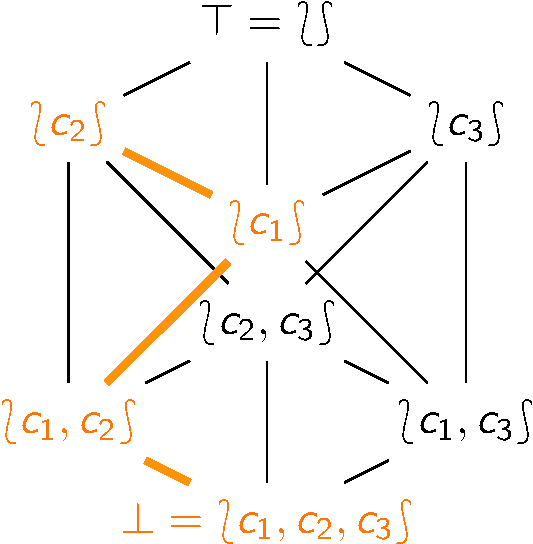
\includegraphics[width=2cm]{img/search-space.pdf}};  
\end{tikzpicture}

\end{center}
\end{textblock*}
\end{frame}

\begin{frame}{Bsp.: Gewichte für Constraint Relationships}
\begin{figure}
\centering
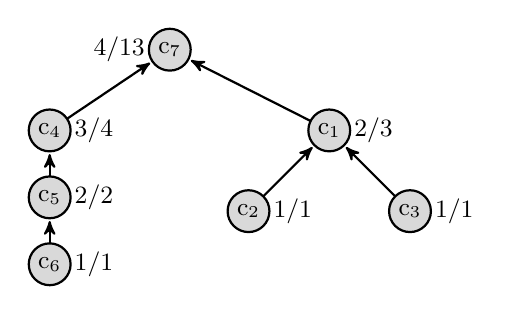
\begin{tikzpicture}[->,>=stealth',shorten >=1pt,auto,node distance=1.45cm,inner sep=1.5pt,outer sep = 0.0pt, thick] 

\tikzstyle{every node}=[font=\small]

\begin{scope}[xshift=-12cm,yshift=0.0cm]
\node[constraint node, xshift=0.6cm, label=west:{\small 4/13}] (1) {$\mathrm{c_7}$};
\node[constraint node, xshift=1cm, label=east:{\small 2/3}] (3)  [below right of=1] {$\mathrm{c_1}$};
\node[constraint node, label=0:{\small 1/1}] (4) [below left of=3] {$\mathrm{c_2}$};
\node[constraint node, label=0:{\small 1/1}] (8) [below right of=3] {$\mathrm{c_3}$};
\node[constraint node, label=0:{\small 3/4}] (5) [below left of=1, xshift=-.5cm] {$\mathrm{c_4}$};
\node[constraint node, node distance=0.85cm, label=0:{\small 2/2}] (6) [below of=5] {$\mathrm{c_5}$};  
\node[constraint node, node distance=0.85cm,label=0:{\small 1/1}] (7) [below of=6] {$\mathrm{c_6}$};  

\path[every node/.style={font=\sffamily\tiny}]
  (3) edge node [right] {} (1)
  (5) edge node [right] {} (1)
  (4) edge node [right] {} (3)
  (8) edge node [right] {} (3) 	
  (6) edge node [right] {} (5)
  (7) edge node [right] {} (6)    
  ;
        
%\draw [rounded corners, black!45,dashed] (-2.0,-0.5) rectangle (0.3,-3.8);
%\node[yshift=-.75cm] (ag1) at (7){ Agent 1};
    
%\draw [rounded corners, black!45,dashed] (0.6,-0.5) rectangle (4.5,-3.8);
%\node[yshift=-2.45cm] (ag2) at (3) { Agent 2};
\end{scope}

\end{tikzpicture}
\caption{Beispiel mit errechneten Gewichten (SPD/TPD)}
\label{fig:combRelGraph}
\end{figure}


%%% Local Variables:
%%% mode: LaTeX
%%% mode: TeX-PDF
%%% mode: TeX-source-correlate
%%% TeX-master: "../quality-quantity-soft-constraints.tex"
%%% End:


\bgroup\abovedisplayskip=-16pt\belowdisplayskip=4pt
\begin{align*}
  \SPDw{}(c) &\textstyle= 1 + \max_{c' \rightarrow^+ c} \SPDw{}(c') 
\\
  \TPDw{}(c) &\textstyle= 1 + \sum_{c' \rightarrow^+ c} \TPDw{}(c')  
\end{align*}
\egroup

\vspace*{1ex} \small \pause 
\begin{itemize}
\item Für Ordnung $P$ über Constraints: PVS $\mathrm{Weighted}(P) = \langle \mathbb{N}, +, \geq, 0 \rangle$
\item $\mathsf{PVS}_{\mathrm{cr}} = \mathit{PVS}\langle P \rangle = \langle \mathcal{M}^{\mathrm{fin}} (P), \mcup, \supseteq_{\mathsf{SPD}}, \lbag \rbag \rangle$
\item $\varphi(\lbag \rbag) = 0$, $\varphi(\lbag c\rbag \mcup C) = \SPDw{}(c) + \varphi(C)$
\end{itemize}



\hfill \cite{Schiendorfer13}
\begin{textblock*}{3cm}[1,1](\textwidth+1cm,\textheight-2.7cm)
%\textblockcolour{issegrey!20}
\begin{center}
\begin{tikzpicture}[auto,
                    ->,>=stealth',shorten >=1pt,thick,
                    node distance=.7cm,inner sep=5pt, 
                    constraint/.style={circle,fill=black!15,draw,font=\sffamily\small}]
\node[overlay,rectangle callout,callout absolute pointer = {(-2,-1)},
     draw=isseorange!50,fill=white] at (0,0) {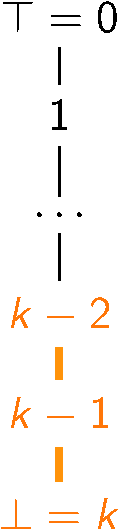
\includegraphics[width=.6cm]{img/search-space-weighted.pdf}};  
\end{tikzpicture}
\end{center}
\end{textblock*}
\end{frame}
%
%\begin{frame}{PVS und Morphismen} \small
%Etwas systematischer \ldots 
%\begin{itemize}
%\item $\mathsf{PVS}_{\mathrm{cr}} = \mathit{PVS}\langle P \rangle = \langle \mathcal{M}^{\mathrm{fin}} (P), \mcup, \supseteq_{\mathsf{SPD}}, \lbag \rbag \rangle$
%\item PVS-Homomorphismus $\varphi : \mathsf{PVS}_{\mathrm{cr}} \to  \mathsf{PVS}_{\mathrm{weighted}}$ \pause 
%\begin{itemize}
%\item[-] $\varphi(\top_{\mathrm{cr}}) = \top_{\mathrm{weighted}}$ \pause 
%\item[-] $\varphi(m \cdot_{\mathrm{cr}} n) = \varphi(m) \cdot_{\mathrm{weighted}} \varphi(n)$ \pause 
%\item[-] $m \leq_{\mathrm{cr}} n \rightarrow \varphi(m) \leq_{\mathrm{weighted}} \varphi(n)$ \pause 
%\end{itemize}
%
%\vspace*{2ex}
%
%\item Beispiel: $\varphi(\lbag \rbag) = 0$, $\varphi(\lbag c\rbag \mcup C) = \SPDw{}(c) + \varphi(C)$
%
%\vspace*{2ex}
%
%\pause 
%\item Warum überhaupt Morphismen?
%\begin{itemize}
%\item[-] Ordnung soll bewusst totalisiert werden
%\item[-] Datentyp $xy$ (z.B. Mengen) wird von Solver/Algorithmus nicht unterstützt
%\item[-] $\rightarrow$ Benutzer interessiert \alert{nicht} konkrete Datenstruktur sondern nur die Erhaltung der gewünschten Ordnung
%\end{itemize}
%\end{itemize}
%%\begin{center}
%%\begin{tikzpicture}
%%  \matrix (m) [matrix of math nodes,row sep=3em,column sep=4em,minimum width=2em,ampersand replacement=\&]
%%  {
%%     \mathit{PVS}\langle P \rangle  \&  \mathit{Weighted}(P) \&  \\
%%  };
%%      
%%  \path[-stealth]
%%    (m-1-1) edge node [above] {$\SPDw{}$} (m-1-2)
%%;
%%
%%\end{tikzpicture}
%%\end{center}
%\begin{textblock*}{3cm}[1,1](\textwidth+.5cm,\textheight-5.3cm)
%%\textblockcolour{issegrey!20}
%\begin{center}
%\begin{tikzpicture}[auto,
%                    ->,>=stealth',shorten >=1pt,thick,
%                    node distance=.7cm,inner sep=2pt,
%                    constraint/.style={circle,fill=black!15,draw,font=\sffamily\small}]
%\node[overlay,rectangle callout,callout absolute pointer = {(-3,0.8)},
%     draw=isseorange!50,fill=white] at (0,.5) {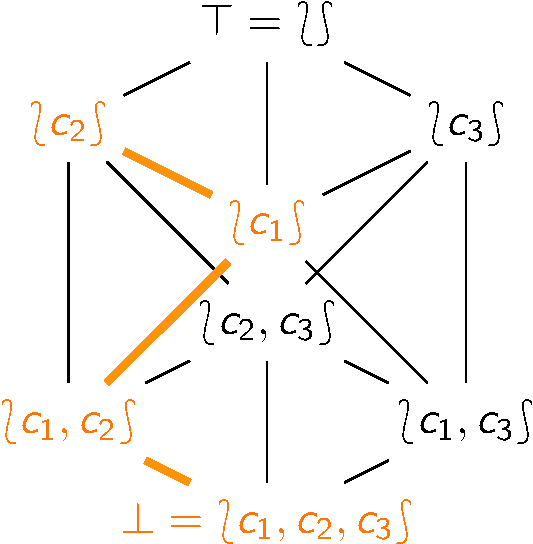
\includegraphics[width=2cm]{img/search-space.pdf}};  
%\end{tikzpicture}
%
%\end{center}
%\end{textblock*}
%\end{frame}


\begin{frame}{Looking for freedom \ldots} \small

\begin{center}
\begin{tikzpicture}[auto,->,
                    >=stealth',shorten >=1pt,thick,
                    node distance=.7cm,inner sep=2pt,
                    constraint/.style={circle,fill=black!15,draw,font=\sffamily\small},
                    bg/.style={shape=rectangle, rounded corners,
    draw, align=center,
    top color=white, bottom color=issegrey!15},
                    pvs/.style={shape=rectangle, rounded corners,
    draw=isseorange!50,fill=white, align=center}]
\node [anchor=west] at (0, .5) {$\mathrm{Cat}: \mathrm{POSet}$};
\node [anchor=west] at (0, -.5) {$\mathrm{Cat}: \mathrm{PVS}$};

\draw [dashed,-] (0,0) -- (11,0);

 \node[bg,text width=2.7cm, text height=1.5cm] at (5,1.6) {};
 \node[anchor=west] at (3.6,2.1) {$P$};
 
\node[constraint node] (1) at (5, 2)                   {$\mathrm{c}_1$};
\node[constraint node] (2) at ($ (1) + (-0.8, -0.8) $) {$\mathrm{c}_2$};  
\node[constraint node] (3) at ($ (1) + ( 0.8, -0.8) $) {$\mathrm{c}_3$};  
%  
\path[every node/.style={font=\sffamily\tiny}]
  (2) edge (1)
  (3) edge (1)
  ;
 
\onslide<2-> { 
\node[pvs,text width=3.5cm,anchor=north west, text height=2.8cm] at (0.5,-1) {};
 \node[anchor=west] at (0.5,-1.3) {$\mathit{Weighted}(P)$};
  \node[anchor=west] at (0.5,-3.6) {$\langle \mathbb{N}, +, \geq, 0 \rangle$};
  
\node[constraint node,label=west:2] (w1) at (2, -2)                   {$\mathrm{c}_1$};
\node[constraint node,label=west:1] (w2) at ($ (w1) + (-0.8, -0.8) $) {$\mathrm{c}_2$};  
\node[constraint node,label=west:1] (w3) at ($ (w1) + ( 0.8, -0.8) $) {$\mathrm{c}_3$};  
\node at (3.5, -2.3) {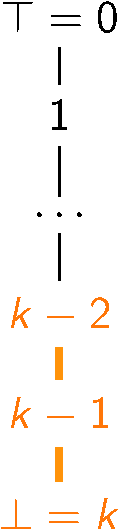
\includegraphics[width=.45cm]{img/search-space-weighted.pdf} }; 

%  
\path[every node/.style={font=\sffamily\tiny}]
  (w2) edge (w1)
  (w3) edge (w1)
  ;
}

\onslide<3->{
\draw [CornflowerBlue] (5,0.7) -- (2,-1);
\node [CornflowerBlue] at (4.2,-0.5) {$\mu(c) = \SPDw{}(c)$};
}  
 
\onslide<4->{
\node[pvs,text width=4.5cm,anchor=north west, text height=2.8cm] at (5.7,-1) {};
\node[anchor=west] at (5.7,-1.3) {$\mathit{PVS}\langle P \rangle $};
\node[anchor=west] at (5.7,-3.6) {$\langle \mathcal{M}^{\mathrm{fin}} (P), \mcup, \smytheq{P}, \lbag \rbag \rangle$};

\node[constraint node,label=west:$\lbag \mathrm{c}_1 \rbag$] (p1) at (7, -2)                   {$\mathrm{c}_1$};
\node[constraint node,label=east:$\lbag \mathrm{c}_2 \rbag$] (p2) at ($ (p1) + (-0.8, -0.8) $) {$\mathrm{c}_2$};  
\node[constraint node,label=north:$\lbag \mathrm{c}_3 \rbag$] (p3) at ($ (p1) + ( 0.8, -0.8) $) {$\mathrm{c}_3$};  
\node at (9.2, -2.3) {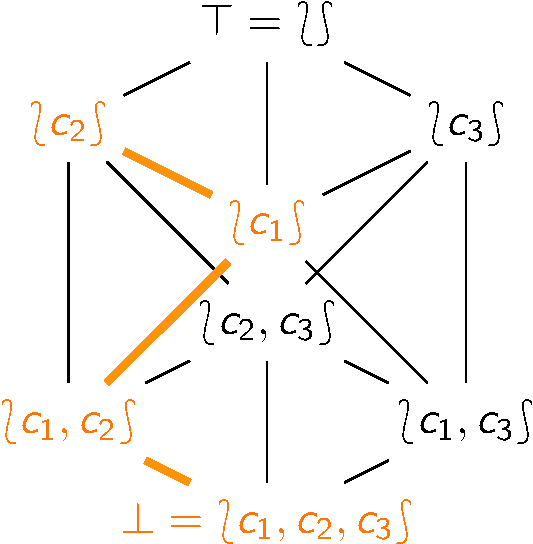
\includegraphics[width=2cm]{img/search-space.pdf} }; 
%  
\path[every node/.style={font=\sffamily\tiny}]
  (p2) edge (p1)
  (p3) edge (p1)
  ;
}
 
\onslide<5->{ 

\draw [isseorange] (5,0.7) -- (8,-1);
\node [isseorange] at (8.7,-0.5) {$\eta(c) = \lbag c \rbag$};
}

\onslide<6->{
\draw [issegrey] (5.7,-2) to [bend right] (4.2,-2);  
\node [issegrey] at (5,-1.5) {$(\SPDw{})^\#$};
}

\onslide<7->{
\draw [issegrey]  (4.2,-2.5) to [bend right] (5.7,-2.5);   
\node [issegrey] at (5,-3) {?};
}
\end{tikzpicture}
\end{center}

\end{frame}

\begin{frame}{Looking for freedom \ldots}
%\begin{itemize}
%\item (Konkrete) Kategorie $\mathsf{POSet}$: 
%\begin{itemize}
%\item[-] Objekte $\rightarrow$ partiell geordnete Mengen
%\item[-] Morphismen $\rightarrow$ monotone Funktionen
%\end{itemize}  
%\end{itemize}
\begin{lemma}[PVS-Freiheit \cite{knapp-schiendorfer2014}]
$\mathit{PVS}\langle P \rangle$ is the free partial valuation structure over the partial order $P$.
\end{lemma}


\begin{center}
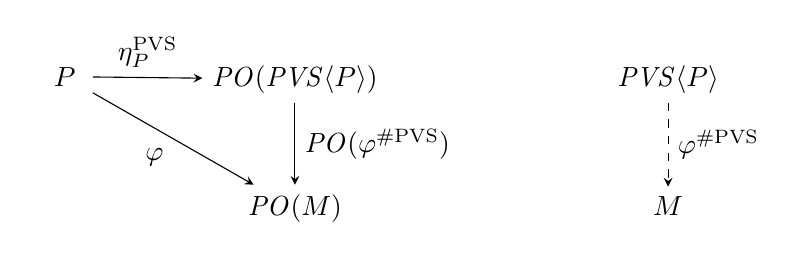
\begin{tikzpicture}
  \matrix (m) [matrix of math nodes,row sep=3em,column sep=4em,minimum width=2em,ampersand replacement=\&]
  {
     P \& \mathit{PO}(\mathit{PVS}\langle P \rangle) \& \& \mathit{PVS}\langle P \rangle \\
      \& \mathit{PO}(M) \& \& M \\};
  \path[-stealth]
    (m-1-1) edge node [above] {$\eta_P^{\mathrm{PVS}}$} (m-1-2)
            edge node [below left] {$\varphi$} (m-2-2)
    (m-1-2) edge node [right] {$\mathit{PO}( \varphi^{\# \mathrm{PVS} })$} (m-2-2)
    (m-1-4) edge [dashed] node [right] {$\varphi^{\# \mathrm{PVS} }$} (m-2-4)
;
\end{tikzpicture}
\end{center}

\cemph{Freie Konstruktionen}

\begin{itemize}
\item no junk
\item no confusion
\end{itemize}
\end{frame}

\begin{frame}[fragile]{Morphismen in MiniBrass}
\begin{lstlisting}
% aus Bibliothek
morph ConstraintRelationships -> WeightedCsp: ToWeighted = 
  params {
    k = 'mbr.nScs * max(i in 1..mbr.nScs) (mbr.weights[i]) ';
    weights = calculate_cr_weights;
  } in id; % "in" denotes the function applied to each soft constraint 
\end{lstlisting}
\begin{lstlisting}   
PVS: cr1 = new ConstraintRelationships("cr1") {
   soft-constraint c1: 'x + 1 = y';
   soft-constraint c2: 'z = y + 2';
   soft-constraint c3: 'x + y <= 3';
   
   crEdges : '[| mbr.c2, mbr.c1 | mbr.c3, mbr.c1 |]';
   useSPD: 'false' ;
}; 
solve ToWeighted(cr1);
\end{lstlisting}
\begin{Verbatim}[fontsize=\small]
Solution: x = 1; y = 2; z = 1
Valuations: overall = 1
\end{Verbatim}
\begin{textblock*}{3cm}[1,1](\textwidth+0.5cm,\textheight+0.3cm)
%\textblockcolour{issegrey!20}
\begin{center}
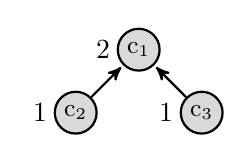
\begin{tikzpicture}[auto,
                    ->,>=stealth',shorten >=1pt,thick,
                    node distance=.7cm,inner sep=2pt,
                    constraint/.style={circle,fill=black!15,draw,font=\sffamily\small}]
\node[constraint node,label=west:2] (1) at (0, 0)                   {$\mathrm{c}_1$};
\node[constraint node,label=west:1] (2) at ($ (1) + (-0.8, -0.8) $) {$\mathrm{c}_2$};  
\node[constraint node,label=west:1] (3) at ($ (1) + ( 0.8, -0.8) $) {$\mathrm{c}_3$};  
%  
\path[every node/.style={font=\sffamily\tiny}]
  (2) edge (1)
  (3) edge (1)
  ;
  

\end{tikzpicture}
\begin{Verbatim}[fontsize=\small]
c1: 'x + 1 = y';
c2: 'z = y + 2';
c3: 'x + y <= 3';   
\end{Verbatim}

\end{center}
\end{textblock*}

\end{frame}

\begin{frame}[fragile]{PVS-Kombinationen: Pareto} \small
Mit PVSs $M$ und $N$ können wir das direkte Produkt $M \times N$ 
\[
(m, n) \leq_{M \times N} (m', n') \leftrightarrow m \leq_M m' \wedge n \leq_N n'
\]
bilden. Entspricht der \emph{Pareto}-Ordnung
\begin{lstlisting}
% in MZN-file: var 1..10: x; var 1..10: y;
PVS: cfn1 = new CostFunctionNetwork("cfn1") {
   soft-constraint c1: 'y' ;
   k : '20';
}; 

PVS: cfn2 = new CostFunctionNetwork("cfn2") {
   soft-constraint c1: 'x' ;
   k : '20';
}; 

solve cfn1 pareto cfn2; % returns x = 1, y = 1
\end{lstlisting}
\end{frame}

\begin{frame}[fragile]{PVS-Kombinationen: Lex}
Außerdem das \alert{lexikographische} Produkt $M \ltimes N$ 
\[
(m, n) \leq_{M \ltimes N} (m', n') \leftrightarrow (m <_M m') \vee (m = m' \wedge n \leq_N n')
\]
Ermöglicht strikte Hierarchien
\begin{lstlisting}
% in MZN-file: var 1..3: x; var 1..3: y;
PVS: cfn1 = new CostFunctionNetwork("cfn1") {
   soft-constraint c1: 'x' ;
   soft-constraint c2: '3 - y' ;
   k : '20';
}; 
PVS: cfn2 = new CostFunctionNetwork("cfn2") {
   soft-constraint c1: 'y' ;
   soft-constraint c2: '3 - x' ;
   k : '20';
};
solve cfn1 lex cfn2; % returns x = 1, y = 3
% dually cfn2 lex cfn1 yields x = 3, y = 1 
\end{lstlisting}
\end{frame}


%

\begin{frame}[fragile]{Mentor Matching}

\textbf{Ziel}: Teile Mentees (z.B. Studenten) Mentoren zu (z.B. Firmen), sodass
\begin{itemize}
\item Studenten sind sehr zufrieden mit ihren Mentoren
\item Firmen sind mit ihren Mentees ebenfalls zufrieden
\item Zweiseitige Präferenzen
\end{itemize}

\vspace*{2ex}

Bisher klingt das wie ein typisches \emph{Stable Matching}-Problem, aber:

\begin{itemize}
\item Es gibt keine 1:1 Abbildung (Firmen betreuen mehrere Studenten)
\item Zusätzliche Constraints sind vorhanden:
\begin{itemize}
\item[-] Jede Firme betreut zumindest $l$, höchstens aber $u$ Studenten
\item[-] Die Anzahl betreuter Studenten \emph{sollten} ungefähr gleich sein pro Firma (Fairness)
\item[-] Studenten, die eine Firma ``verachten'', sollen nicht gezwungen werden (\emph{harter Ausschluss} von Lösungen)
\end{itemize}
\end{itemize}
\end{frame}


\begin{frame}[fragile]{Mentor Matching: Beispiel}
\begin{center}
\tikzset{onslide/.code args={<#1>#2}{%
  \only<#1>{\pgfkeysalso{#2}}
}}

\tikzstyle{highlight}=[isseorange,ultra thick]
\tikzstyle{highlight2}=[CornflowerBlue,ultra thick,rounded corners]
\tikzstyle{defaultStyle}=[white,ultra thick,rounded corners]

\tikzstyle{impo}=[dashed]
\begin{tikzpicture}[every node/.style={
anchor=base,
%text depth=.5ex,
%text height=2ex,
%minimum height=2ex,
align=center,
rectangle,
text width=2em
}]
\matrix (magic) [nodes in empty cells, ampersand replacement=\&,row sep=0.4cm,column sep=1.5cm]
{
\node[draw,defaultStyle, onslide={<3->{highlight2}}](s1){
\includegraphics[width=\textwidth]{img/businessman.png}}; \& \& \& \node[text width=4em, defaultStyle, draw, onslide={<3->{highlight2}}](c1) {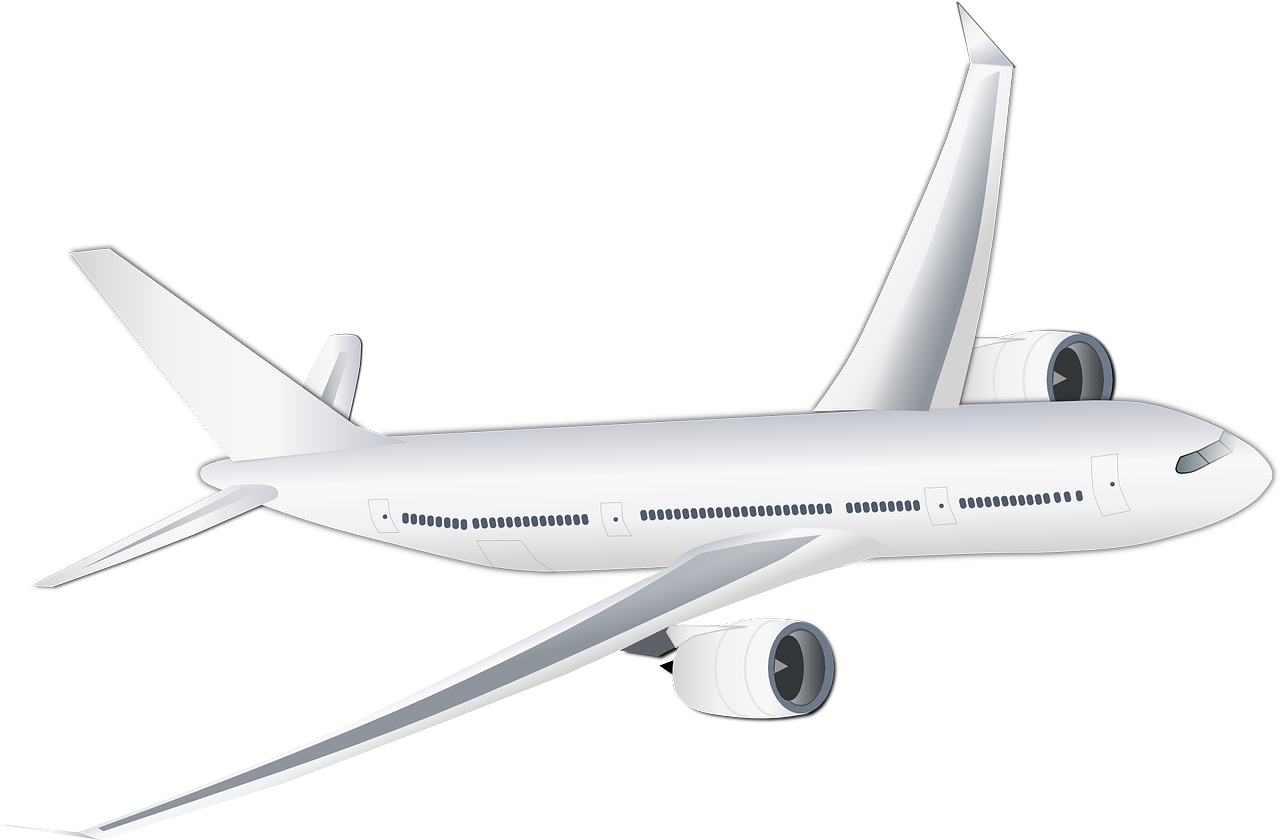
\includegraphics[width=\textwidth]{img/airplane.png}}; \\
\node(s2){
\includegraphics[width=\textwidth]{img/woman.png}};       \& \& \& \node(c2) {
\includegraphics[width=2\textwidth]{img/logistics.png}}; \\
\node(s3){
\includegraphics[width=\textwidth]{img/man.png}};         \& \& \& \node(c3) {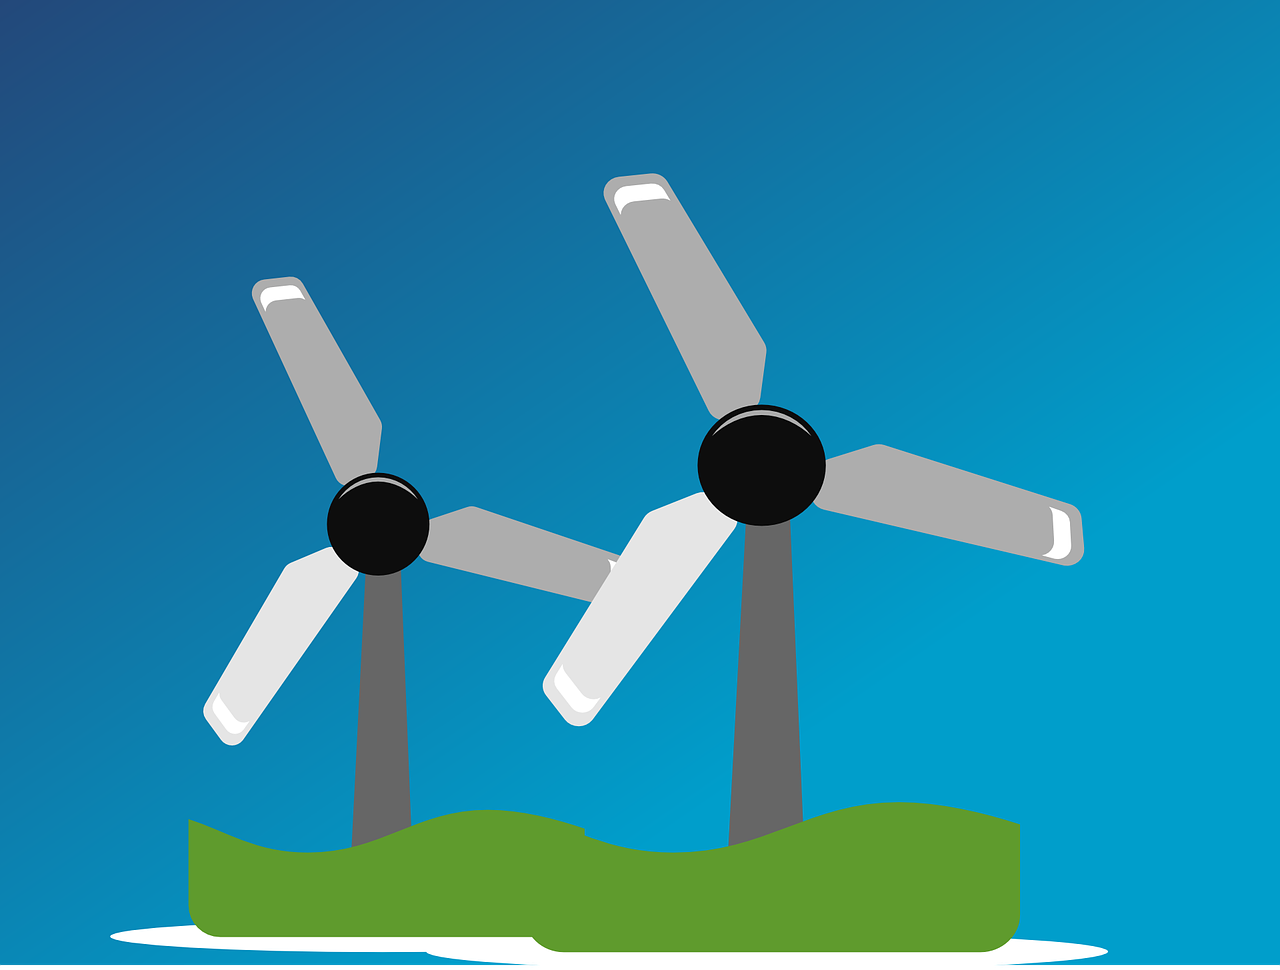
\includegraphics[width=2\textwidth]{img/enrgy.png}}; \\
\node[defaultStyle, draw, onslide={<3->{highlight2}}](s4){
\includegraphics[width=\textwidth]{img/woman2.png}};      \& \\
};

\draw[onslide={<2->{highlight}}] (s1) -- (c1);
\draw[] (s1) -- (c2);

\draw[onslide={<2->{highlight}}] (s2) -- (c1);
\draw[] (s2) -- (c3);

\draw[onslide={<2->{highlight}}] (s3) -- (c2);

\draw[onslide={<2->{highlight}}] (s4) -- (c3);
\draw[] (s4) -- (c2);
%
%\draw[onslide={<1-2>{highlight}}] (z) -- (3);
%\draw[onslide={<3>{highlight}}] (z) -- (2);
%
%\draw[onslide={<1-2>{highlight}}] (t) -- (2);
%\draw[] (t) -- (1);
%\draw[onslide={<3>{highlight}}] (t) -- (5);
%\draw[] (t) -- (3);
%\draw[] (t) -- (4);
%\draw[onslide={<1>{highlight}}] (u) -- (4);
%\draw[] (u) -- (3);
%\draw[] (u) -- (5);
%\draw[] (u) -- (6);
\end{tikzpicture}
\end{center}
\onslide<2->{Diese \alert{Zuweisung} respektiert die studentischen Präferenzen  (Kanten) \onslide<3->{ignoriert aber die  {\color{CornflowerBlue} Firmenpräferenzen}.}}
\onslide<4->{\tiny OK, es ist nicht wirklich ein \emph{Matching} da Firmen mehr als einen Studenten betreuen \ldots }
\end{frame}

\begin{frame}[fragile]{Mentor Matching: Constraint-Modell}
\begin{lstlisting}
int: n; set of int: STUDENT = 1..n;
int: m; set of int: COMPANY = 1..m;

% assign students to companies
array[STUDENT] of var COMPANY: worksAt;


int: minPerCompany = 1; int: maxPerCompany = 3;
constraint global_cardinality_low_up ( 
           worksAt, [c | c in COMPANY], 
           [minPerCompany | c in COMPANY], 
           [maxPerCompany | c in COMPANY]); 
           
solve 
search pvs_BAB();
\end{lstlisting}
\end{frame}

\begin{frame}[fragile]{Mentor Matching: FMSOFT Instanz}
\begin{lstlisting}
% fmsoft2016.mzn

n = 5; % students
m = 3; % companies

% student names for better readability 
int: raubholz = 1;
int: schraubale = 2;
int: meerfluss = 3; 
int: gleich = 4; 
int: lustig = 5; 

% company names 
int: delphi = 1;
int: cupgainini = 2;
int: youthlab = 3;

\end{lstlisting}

\end{frame}

\begin{frame}[fragile]{Mentor Matching: Präferenzen}
\begin{lstlisting}
PVS: students = new ConstraintRelationships("students") {
   soft-constraint raubholzdelphi: 'worksAt[raubholz] = delphi';
   soft-constraint raubholzyouthlab: 'worksAt[raubholz] = youthlab';
   soft-constraint gleichcupg: 'worksAt[gleich] = cupgainini';
   
   crEdges : '[| mbr.raubholzyouthlab, mbr.raubholzdelphi | 
                 mbr.gleichcupg, mbr.raubholzdelphi |]';
   useSPD: 'true' ;
}; 

PVS: companies = new ConstraintRelationships("companies") {
   soft-constraint delphi_meer: 'worksAt[meerfluss] = delphi';
   soft-constraint delphi_gleich: 'worksAt[gleich] = delphi';
   soft-constraint youthlab: 'worksAt[lustig] = youthlab';
   
   crEdges : '[| mbr.delphi_meer, mbr.delphi_gleich |]';
   useSPD: 'true' ;
}; 

\end{lstlisting}
\end{frame}

\begin{frame}[fragile]{Mentor Matching: Verhalten I}
\begin{lstlisting}
solve ToWeighted(students) lex ToWeighted(companies);
\end{lstlisting}
\begin{Verbatim}[fontsize=\small]
Intermediate solution:worksAt = [3, 2, 1, 1, 1]
Valuations: pen_companies = 1; pen_students = 3
----------
Intermediate solution:worksAt = [1, 2, 3, 1, 1]
Valuations: pen_companies = 2; pen_students = 2
----------
Intermediate solution:worksAt = [1, 3, 1, 2, 1]
Valuations: pen_companies = 3; pen_students = 1
----------
Intermediate solution:worksAt = [1, 1, 1, 2, 3]
Valuations: pen_companies = 2; pen_students = 1
----------
==========
\end{Verbatim}

\end{frame}

\begin{frame}[fragile]{Mentor Matching: Verhalten II}
\begin{lstlisting}
solve ToWeighted(companies) lex ToWeighted(students);
\end{lstlisting}
\begin{Verbatim}[fontsize=\small]
Intermediate solution:worksAt = [3, 2, 1, 1, 1]
Valuations: pen_companies = 1; pen_students = 3
----------
Intermediate solution:worksAt = [2, 1, 1, 1, 3]
Valuations: pen_companies = 0; pen_students = 4
----------
Intermediate solution:worksAt = [1, 2, 1, 1, 3]
Valuations: pen_companies = 0; pen_students = 2
----------
==========
\end{Verbatim}

\end{frame}


\begin{frame}[fragile]{Mentor Matching: WS 15/16}
\begin{itemize}
\item Präferenzen aus E-Mails vom WS 15/16 gesammelt

\begin{parchment}
\begin{verbatim}
"the favorites":
1. JuneDied-Lynx- HumanIT
2. Cupgainini
 
"I could live with that":
3. Seamless-German
4. gsm systems
5. Yiehlke
 
"I think, we won't be happy":
6. APS
7. Delphi Databases
\end{verbatim} 
\end{parchment}
\end{itemize}
\end{frame}

\begin{frame}[fragile]{Mentor Matching: WS 15/16}
\begin{itemize}
\item Priorität zu \alert{Studenten}
\begin{itemize}
\item[-] Was sollen Firmen schon mit unzufriedenen Mentees anfangen?
\end{itemize}
\item Suchraum: 7 Firmen für 16 Studenten $\rightarrow 7^{16} = 3.3233 \cdot 10^{13}$
\vspace*{2ex}
\item Führte zu einem Constraint-Problem mit
\begin{itemize}
\item[-] 77 student. Präferenzen (Soft Constraints) von 16 Studenten
\item[-] insgesamt 114 Soft Constraints (37 Firmenpräferenzen) 
\end{itemize}

\vspace*{2ex}

\item \emph{Bewiesen} optimale Lösung
\begin{itemize}
\item[-] 6 Minuten Lösungszeit
\end{itemize}
\end{itemize}
\end{frame}



\begin{frame}[fragile]{Prüfungstermine}

\textbf{Ziel}: Weise Prüfungstermine an Studenten zu, sodass
\begin{itemize}
\item Jeder Student stimmt seinem Termin zu 
\item Die Anzahl verschiedener Termine wird minimiert (um das Zeitinvestment der Dozenten zu schonen)
\end{itemize}

%\vspace*{2ex}
%\begin{parchment}
\begin{center}
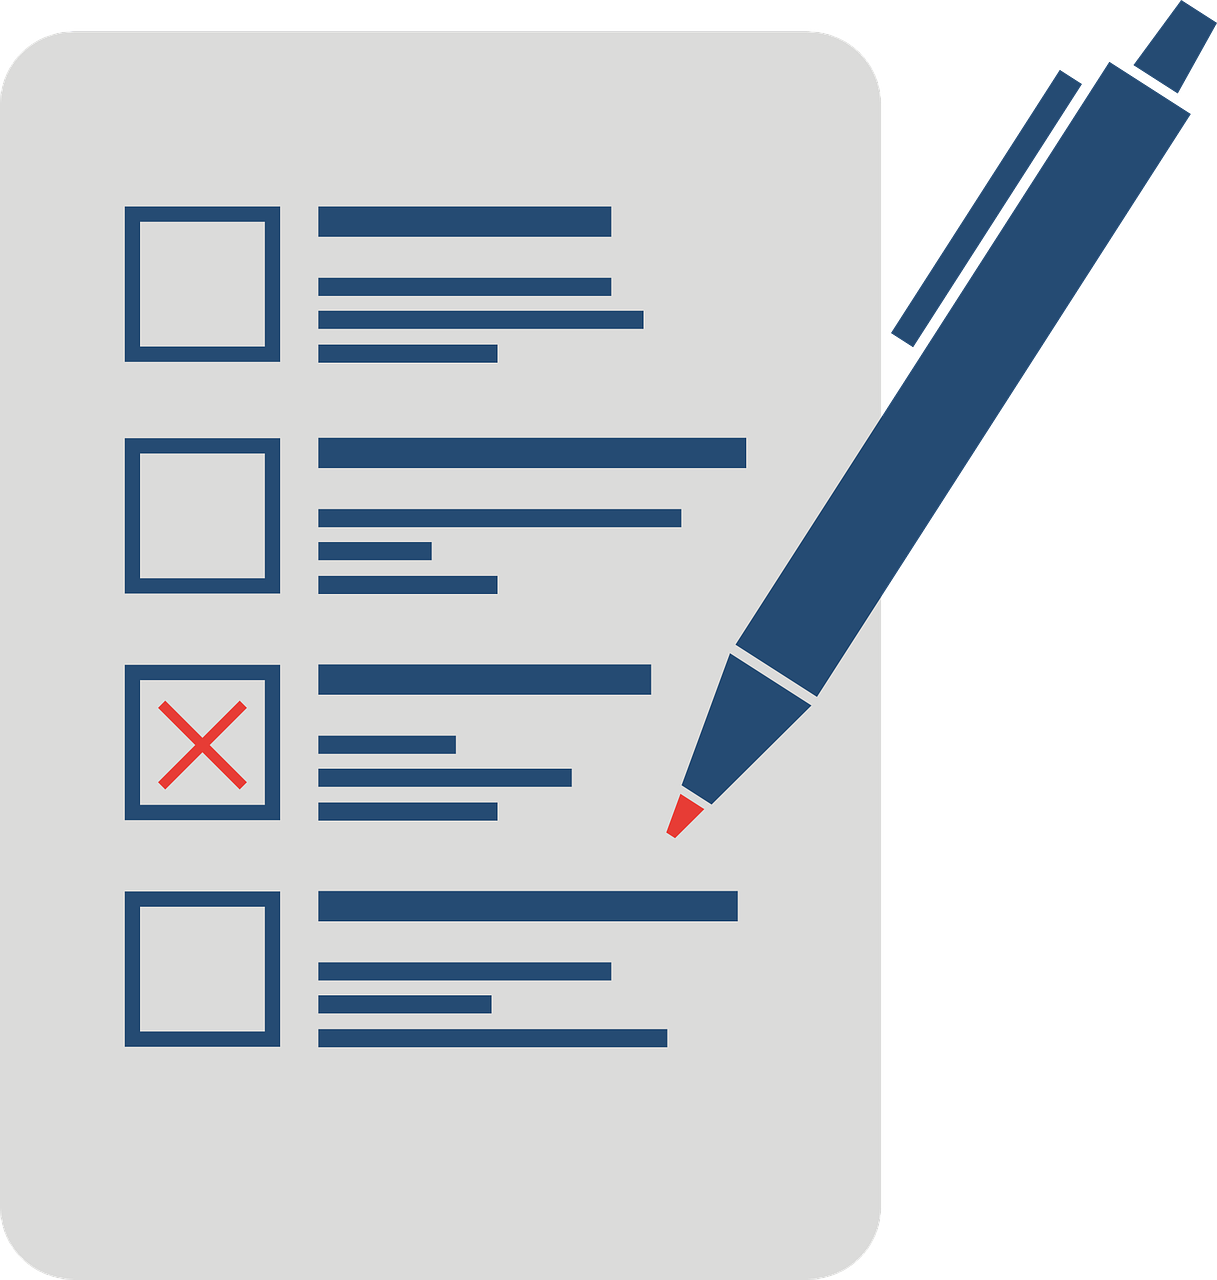
\includegraphics[width=.15\textwidth]{img/voting.png}
\hspace*{4ex}
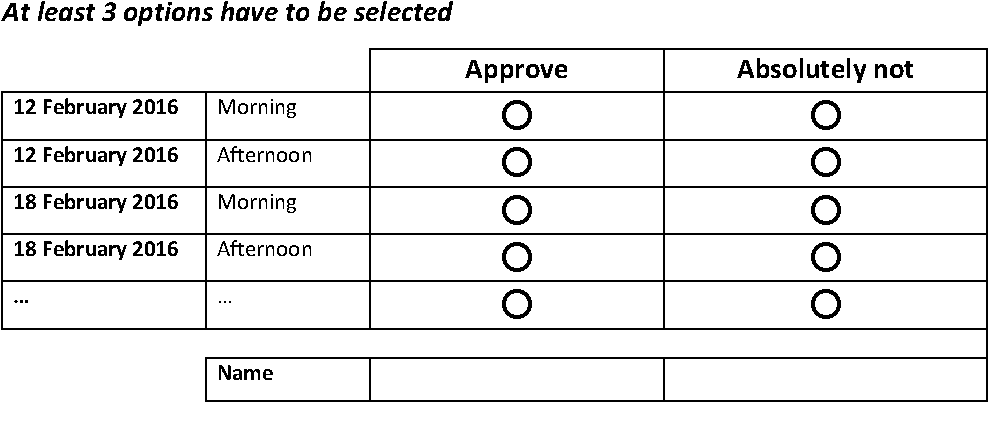
\includegraphics[width=.5\textwidth]{img/Voting.pdf}
\end{center}
%\end{parchment}

\begin{itemize}
\item Kein studentischer Wunsch sollte höher gewichtet werden
\item Prüfungsplan ist eine gemeinsame Entscheidung

\end{itemize}
\end{frame}

\begin{frame}[fragile]{Prüfungstermine: Constraint-Modell}
\begin{lstlisting}
% Exam scheduling example with just a set of 
% approved dates and *impossible* ones
include "globals.mzn";
include "soft_constraints/soft_constraints.mzn";

int: n; set of int: STUDENT = 1..n; 
int: m; set of int: DATE = 1..m;
array[STUDENT] of set of DATE: possibles;
array[STUDENT] of set of DATE: impossibles;

% the actual decisions
array[STUDENT] of var DATE: sd;

int: minPerSlot = 0; int: maxPerSlot = 4;
constraint global_cardinality_low_up(sd % minPerSlot, maxPerSlot
constraint forall(s in STUDENT) (not (sd[s] in impossibles[s])); 
 
\end{lstlisting}
\end{frame}

\begin{frame}[fragile]{Prüfungstermine: Präferenzen}

\begin{lstlisting}
include "../defs.mbr";
PVS: students = new WeightedCsp("students") {
   k: '100';
   soft-constraint raubholz:   'sd[raubholz] in {monday, tuesday}';   
   soft-constraint schraubale: 'sd[schraubale] in {tuesday, wednesday}';
   soft-constraint meerfluss:  'sd[meerfluss] in {tuesday}';
   soft-constraint gleich:   'sd[gleich] in {monday, tuesday}';
   soft-constraint lustig:     'sd[lustig] in {monday, wednesday}';
   % hard by weight (less than bottom)
   soft-constraint lustig-urlaub: 'sd[lustig] != tuesday'
                                :: weights('101'); 
}; 
PVS: teachers = new CostFunctionNetwork("teachers") {
   soft-constraint scheduledDates: 'scheduledDates';
}; 
solve students lex teachers;
\end{lstlisting}
\begin{Verbatim}[fontsize=\small]
Scheduled: [1, 2, 2, 1, 1], Distinct dates: 2
Valuations: mbr_overall_students = 0; mbr_overall_teachers = 2
\end{Verbatim}
\end{frame}


\begin{frame}[fragile]{Prüfungstermine: WS 15/16}

\begin{itemize}
\item Gesammelte Präferenzen von 33 Studenten
\item 12 mögliche Termine (6 Tage, Vormittag und Nachmittag)
\begin{itemize}
\item[-] \emph{Approval}-Menge 
\item[-] \emph{Impossible}-Menge
\end{itemize}

\vspace*{2ex}

\item Aggregiert via Wahl durch Zustimming (\alert{Approval voting}), hat ansprechende wahltheoretische Eigenschaften (Arrow)!
\item Höchstens 4 pro Termin

\item Sofort (61 msec) wurde eine optimale Lösung gefunden, die
\begin{itemize}
\item[-] von \emph{jedem} Student Zustimmung erhält
\item[-] Mit der Minimalanzahl von 9 Terminen auskommt
\end{itemize}
\item Verwendete Strategie (natürlich, \ldots):
\end{itemize}
\begin{lstlisting}
solve students lex teachers;% pro students
\end{lstlisting}
\end{frame}

\begin{frame}[fragile]{Energiefallstudie: Unit Commitment}

\textbf{Ziel}: Weise Kraftwerken Produktion zu, sodass
\begin{itemize}
\item Der Bedarf gedeckt wird
\item Steuerungsvorlieben (ökonomische Leistungsbereiche, \ldots) eingehalten werden
\end{itemize}
\fontsize{8pt}{7.2}\selectfont
\tikzset{
   main node/.style={rectangle,
                     rounded corners,
   					 fill=black!15,
   					 draw,
   					 minimum width=3.5em,
   					 text centered,
                     inner sep=2.5pt,	 
   					 font=\sffamily
   					},
   treestyle/.style={rectangle,fill=black!15,draw,font=\sffamily},
   constraint/.style={circle,fill=black!15,draw,font=\sffamily\small},
   constraint_satisfied/.style = {constraint, fill=white},
   constraint_violated/.style = {constraint, fill=black!25},
}

\begin{figure}[t]
\centering
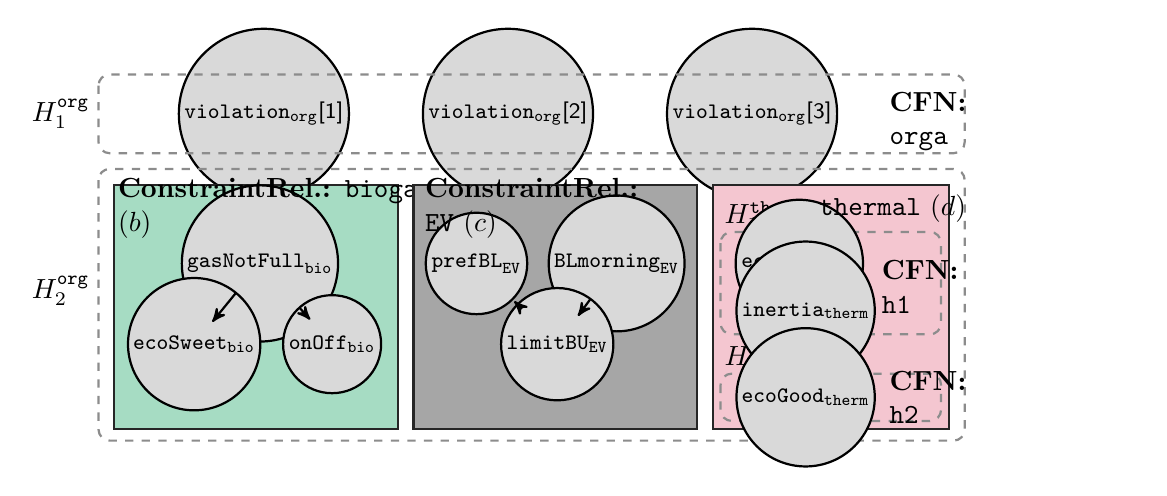
\begin{tikzpicture}[->,>=stealth',shorten >=1pt,auto,node distance=1.45cm,inner sep=1.5pt,outer sep = 0.0pt, thick] 
%\tikzstyle{every node}=[font=\tiny]
\begin{scope}[xshift=-6.0cm,yshift=-4.0cm]
\node[main node, style={font=\sffamily\footnotesize}] at (0.1,1.5) {\minMaxViolation[1]};
\node[main node, style={font=\sffamily\footnotesize}] at (3.2,1.5) {\minMaxViolation[2]};
\node[main node, style={font=\sffamily\footnotesize}] at (6.3,1.5) {\minMaxViolation[3]};

\draw [rounded corners,dashed,black!45] (-2,2) rectangle (9.0,1);
\node[text width=3cm, anchor=west, right] at (-2.9, 1.5) { \hLevelOrg{1} };
\draw [rounded corners,dashed,black!45] (-2,0.8) rectangle (9.0,-2.65);
\node[text width=4cm, anchor=west, right] at (-2.9, -0.75) { \hLevelOrg{2} };

% bio
\draw [black!85,fill=forestgreen!35] (-1.8,0.6) rectangle (1.8,-2.5);
\node[main node, style={font=\sffamily\footnotesize}] (5) at (0.05,-0.4) {\gasFull};
\node[main node, style={font=\sffamily\footnotesize}] (6) [below left of=5,xshift=5.4] {\ecoSweet};
\node[main node, style={font=\sffamily\footnotesize}] (7) [below right of=5,xshift=-3.1] {\onOff};
%\node[main node, style={font=\sffamily\footnotesize},double] (hardConstraint) [below left of=7,xshift=-3.1,yshift=7] {$\mathsf{maxProd}$};
\node[text width=4cm, anchor=west, left] at (2.3, 0.3) { \textbf{ConstraintRel.:}  $\mathtt{\biogas}$ $(b)$ };
%\node[text width=2cm, anchor=west, left] at (0.4, 0.3) { CR \textsc{TPD} };

% EV
\draw [black!85,fill=black!35] (2.0,0.6) rectangle (5.6,-2.5);
\node[main node, style={font=\sffamily\footnotesize}] (3) at (2.80,-0.4) {\prefBatteryLevel};
\node[main node, style={font=\sffamily\footnotesize}] (4) at (4.58,-0.4)  {\earlyBird};
\node[main node, style={font=\sffamily\footnotesize}] (8) [below right of=3] {\limitBatteryUsage};
\node[text width=3cm, anchor=west, left] at (5.2, 0.3) { \textbf{ConstraintRel.:}  $\mathtt{\ev}$ $(c)$ };
%\node[text width=2cm, anchor=west, left] at (4.3, 0.3) { CR };
%\node[text width=1cm, anchor=east, left] at (5.3, -2.3) { \textsc{SPD} };

% thermal
\draw [black!85,fill=thermicred!25] (5.8,0.6) rectangle (8.8,-2.5);
\draw [rounded corners,dashed,black!45] (5.9,0) rectangle (8.7,-1.3);
\node[text width=4cm, anchor=west, right] at (5.9, 0.2) { \hLevelThermal{1} };
\draw [rounded corners,dashed,black!45] (5.9,-1.8) rectangle (8.7,-2.4);
\node[text width=4cm, anchor=west, right] at (5.9, -1.6) { \hLevelThermal{2} };
\node[main node, style={font=\ttfamily\footnotesize}] (10) at (6.9,-0.4) {\ecoOpt};
\node[main node, node distance=0.85cm, style={font=\sffamily\footnotesize}] (11) at (6.98,-1.0) {\inertia};
\node[main node, node distance=0.85cm, style={font=\sffamily\footnotesize}] (12) at (6.98,-2.1) {\ecoGood};
\node[text width=4cm, anchor=west, right] at (7.1, 0.3) { $\mathtt{\thermal}$ $(d)$ };

\node[text width=2cm, anchor=west, left] at (10, -0.7) { \textbf{CFN:} \\ $\mathtt{h1}$ };

\node[text width=2cm, anchor=west, left] at (10.1, -2.1) { \textbf{CFN:} \\ $\mathtt{h2}$ };

\node[text width=2cm, anchor=west, left] at (10.1, 1.4) { \textbf{CFN:} \\ $\mathtt{orga}$ };

\path[every node/.style={font=\sffamily\tiny}]
  (8) edge node [right] {} (3)
  (8) edge node [right] {} (4)
  (6) edge node [right] {} (5)
  (7) edge node [right] {} (5)
;
\end{scope}

% \begin{scope}[xshift=-0.2cm,yshift=-0.9cm]
% \node[text width=9cm,left] at (0.0, 0.0) {%
% \begin{itemize}[itemsep=2pt]
%   \item something interesting
% \end{itemize}
% };
% \end{scope}

\end{tikzpicture}
%\caption{Case study depicting individual and organizational preference specifications in context.}
\label{fig:preferencesCaseStudy}
\end{figure}
  



%%% Local Variables:
%%% mode: LaTeX
%%% mode: TeX-PDF
%%% mode: TeX-source-correlate
%%% TeX-master: "../quality-quantity-soft-constraints.tex"
%%% End:


\end{frame}


\begin{frame}[fragile]{Unit Commitment: Constraint-Modell}
\begin{lstlisting}
int: T = 5; set of int: WINDOW = 1..T;
array[WINDOW] of int: demand = [20, 21, 25, 30, 29];

int: P = 3; set of int: PLANTS = 1..P;

array[PLANTS] of int: pMin  = [12, 5, 7];
array[PLANTS] of int: pMax  = [15, 11, 9];

array[WINDOW, PLANTS] of var 0..15: supply; 
constraint forall(p in PLANTS, w in WINDOW) 
     (supply[w,p] in pMin[p]..pMax[p]);

array[WINDOW] of var int: violation = 
    [ abs( sum(p in PLANTS) (supply[w, p]) - demand[w] ) | w in WINDOW];

solve search pvs_BAB();
\end{lstlisting}
\end{frame}

\begin{frame}[fragile]{Prüfungstermine: Präferenzen I}

\begin{lstlisting}
PVS: orga = new CostFunctionNetwork("Orga") {
    soft-constraint vio_1: 'violation[1]';
    soft-constraint vio_2: 'violation[2]';
    soft-constraint vio_3: 'violation[3]';
    isWorstCase: 'true';
};
PVS: biogas = new ConstraintRelationships("biogas") {
   soft-constraint gasFull: 
     'forall(w in WINDOW) (supply[w,biogas] >= 13)';
   soft-constraint ecoSweet: 
     'forall(w in WINDOW) (supply[w,biogas] >= 14)';
   soft-constraint onOff: 
     'forall(w in 1..T-1) ( 
        abs(supply[w,biogas] - supply[w+1,biogas]) <= 1)';
   
   crEdges : '[| mbr.ecoSweet, mbr.gasFull | mbr.onOff, mbr.gasFull |]';
   useSPD: 'true' ;
}; 
\end{lstlisting}
\end{frame}

\begin{frame}[fragile]{Prüfungstermine: Präferenzen II} \small

\begin{lstlisting}
PVS: ev = new ConstraintRelationships("ev") {...}; 

PVS: therm1 = new CostFunctionNetwork("therm1") {
  soft-constraint ecoOpt: 
    'sum(w in WINDOW) ( abs(supply[w,thermal] - 8) )';
  soft-constraint inertia: 
    'sum(w in 1..T-1) ( abs(supply[w,thermal] - supply[w+1,thermal]))';
};

PVS: therm2 = new CostFunctionNetwork("therm2") {
  soft-constraint ecoGood: 
    'sum(w in WINDOW) ( abs(supply[w,3] - 9) )';
};

solve orga lex ( biogas pareto ev pareto  (therm1 lex therm2) );
\end{lstlisting}
$P_{\mathtt{org}_1} \ltimes (P_{\prosumer{\biogas}} \times P_{\prosumer{\ev}} \times (P_{\prosumer{\thermal}}^1 \ltimes P_{\prosumer{\thermal}}^2))$
\end{frame}


\begin{frame}{Evaluation-Probleme}
Originalprobleme aus der \emph{MiniZinc-Benchmark-Library}; versehen um zusätzliche Soft Constraints als Constraint Preferences

\vspace*{1ex}

\begin{description}
\item[\textbf{Soft N-Queens}] N-Damen mit Zusatzbedingungen (z.B. 1 Dame in der Mitte)
\item[\textbf{Photo Placement}] Platziere Personen auf Foto neben gewünschten anderen (manche lieber als andere)
\item[\textbf{Talent Scheduling}] Plane Szenen und Drehtage; Szenen sollten nicht zu früh beginnen/spät enden; Manche Schauspiele gehen einander lieber aus dem Weg
\item[\textbf{On-call Rostering}] Belegungsplan für Bereitschaftsdienste unter arbeitsrechtlichen Bedingungen. Präferenzen für/gegen gewissen Daten bzw. Kooperation mit Kollegen
\item[\textbf{Multi-Skilled Project Scheduling}] Weise zeitgebundene Tasks an Agenten mit mehreren Capabilities zu (unter Einhaltung von Präzedenz) -- ähnlich zu ODP/COMBO
\end{description}

\end{frame}

\begin{frame}{Eckdaten}

\begin{table}
\centering
{
\label{tab:resultsSolverComparison}

\begin{tabular}{l|l}
\toprule
Konfigurationen &  16 \\
Probleme & 5 \\
Instanzen & 28 \\
Solver & 7 \\
\midrule
\textbf{Versuchte Probleme} & 1793 \\
\textbf{Gelöste Probleme} & 1289 (71.9\%) \\
\textbf{Optimal gelöste Probleme} & 1250 (69.7\%) \\
\bottomrule
\end{tabular}

}
\end{table}
\end{frame}

\begin{frame}{Kompatibilität}
\begin{table}
\centering
{
\small
\label{tab:resultsSolverComparison}

\begin{tabular*}{\textwidth}{@{\extracolsep{\fill} }lcccccc}
\toprule
 & Gecode & JaCoP & OR-Tools & Choco & G12 & Toulbar2* \\
\midrule
Free PVS & \checkfull & \checkfull & \checknot & \checknot & \checknot & \checknot \\ 
Constraint Preferences & \checkfull & \checkfull & \checknot & \checknot & \checknot & \checknot \\
Fuzzy CSP & \checkfull & \checkfull & \checkhalf & \checkhalf & \checkhalf & \checkhalf \\
Probabilistic CSP & \checkfull & \checkfull & \checkhalf & \checkhalf & \checkhalf & \checkhalf \\
Max CSP  & \checkfull & \checkfull & \checkfull & \checkfull & \checkfull & \checkfull \\
Weighted CSP  & \checkfull & \checkfull & \checkfull & \checkfull & \checkfull & \checkfull \\
Cost Function Networks  & \checkfull & \checkfull & \checkfull & \checkfull & \checkfull & \checkfull \\
\bottomrule
\end{tabular*}

}
\end{table}

\begin{itemize}
\item \checkfull \ldots voll unterstützt
\item \checkhalf \ldots teils unterstützt durch Morphismen
\item { \checknot \ldots nicht unterstützt }
\item \color{black} * \ldots Dedizierter Soft Constraint Solver
\end{itemize}
\end{frame}

\begin{frame}[fragile]{Solver-Vergleich auf Weighted CSP}
\vspace*{2ex}
\begin{columns}[onlytextwidth]
    \begin{column}{.45\textwidth}
    \centering \hFirst{Klassische Solver}

    \vspace*{1ex}

    
\includegraphics[width=.2\columnwidth]{img/gecode.png}    
    
\includegraphics[width=.2\columnwidth]{img/JACOP.png}
    
    
\includegraphics[width=.2\columnwidth]{img/choco.png}
    
\includegraphics[width=.2\columnwidth]{img/orLogo.png}

    
\includegraphics[width=.5\columnwidth]{img/nictaorg.png}
	
    \end{column}
    \begin{column}{.45\textwidth}
    \centering \hSecond{Soft Constraint Solver} (Toulbar2)

    \vspace*{1ex}
    
    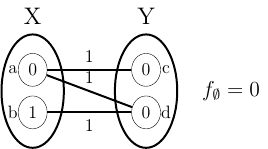
\includegraphics[scale=0.4]{img/toulbar2-0.png}
    \end{column}
\end{columns}
\begin{lstlisting}
solve ToWeighted(constraintPrefs1);
\end{lstlisting}
\begin{parchment}[Evaluationsfrage]
Wie schnell und effektiv (hinsichtlich des Findens von Optima) können Weighted-Instanzen durch klassische Constraint Solver gegenüber dedizierten Soft Constraint Solvern gelöst werden?
\end{parchment}
\end{frame}

\begin{frame}{Solver-Vergleich auf Weighted CSP I}
\vspace*{2ex}
\begin{table}
\centering
{
\scriptsize
\label{tab:resultsSolverComparison}

\begin{tabular*}{\textwidth}{@{\extracolsep{\fill} }ld{1.5}cd{1.5}d{1.1}d{1.1}}
\toprule
\multicolumn{1}{c}{Solver} & \multicolumn{1}{c}{Time (secs)} 
          & \multicolumn{1}{c}{\# Wins}
          & \multicolumn{1}{c}{Objective} 
          & \multicolumn{1}{c}{\% Solved} & \multicolumn{1}{c}{\% Optimal} \\
\midrule
\multicolumn{2}{l}{MSPSP (8 instances)  }   \\
\midrule
   Gecode & 0.32 \quad (1.00)& 8 & 2.50 \quad (0.00) & 100.00 & 100.00 \\
   G12 & 0.32 \quad (1.01)& 0 & 2.50 \quad (0.00) & 100.00 & 100.00 \\
   OR-Tools & 0.33 \quad (1.05)& 0 & 2.50 \quad (0.00) & 100.00 & 100.00 \\
   JaCoP & 0.52 \quad (1.73)& 0 & 2.50 \quad (0.00) & 100.00 & 100.00 \\
   Choco & 0.70 \quad (2.46)& 0 & 2.50 \quad (0.00) & 100.00 & 100.00 \\
   Toulbar2 & 312.56 \quad (1052.07)& 0 & 29.13 \quad (26.63) & 0.00 & 0.00 \\
\midrule
\multicolumn{2}{l}{On-Call Rostering (7 instances)  }   \\
\midrule
   Toulbar2 & 40.73 \quad (1.44)& 3 & 1.57 \quad (0.00) & 100.00 & 100.00 \\
   OR-Tools & 275.23 \quad (5.55)& 2 & 3.71 \quad (2.14) & 100.00 & 57.14 \\
   Gecode & 275.23 \quad (5.54)& 1 & 4.57 \quad (3.00) & 100.00 & 57.14 \\
   G12 & 276.36 \quad (5.63)& 1 & 5.57 \quad (4.00) & 100.00 & 57.14 \\
   JaCoP & 276.63 \quad (5.86)& 0 & 5.14 \quad (3.57) & 100.00 & 57.14 \\
   Choco & 276.72 \quad (6.26)& 0 & 5.14 \quad (3.57) & 100.00 & 57.14 \\
\midrule
\multicolumn{2}{l}{Photo Placement (3 instances)  }   \\
\midrule
   Toulbar2 & 0.80 \quad (1.11)& 0 & 13.33 \quad (0.00) & 100.00 & 100.00 \\
   Choco & 0.83 \quad (1.21)& 2 & 25.00 \quad (11.67) & 100.00 & 100.00 \\
   OR-Tools & 1.49 \quad (1.71)& 1 & 13.33 \quad (0.00) & 100.00 & 100.00 \\
   JaCoP & 3.18 \quad (3.61)& 0 & 13.33 \quad (0.00) & 100.00 & 100.00 \\
   Gecode & 22.24 \quad (21.62)& 0 & 13.33 \quad (0.00) & 100.00 & 100.00 \\
   G12 & 27.40 \quad (29.62)& 0 & 13.33 \quad (0.00) & 100.00 & 100.00 \\
\bottomrule
\end{tabular*}

}
\end{table}

\end{frame}

\begin{frame}{Solver-Vergleich auf Weighted CSP II}
\begin{table}
\centering
{
\scriptsize
\label{tab:resultsSolverComparison}

\begin{tabular*}{\textwidth}{@{\extracolsep{\fill} }ld{1.5}cd{1.5}d{1.1}d{1.1}}
\toprule
\multicolumn{1}{c}{Solver} & \multicolumn{1}{c}{Time (secs)} 
          & \multicolumn{1}{c}{\# Wins}
          & \multicolumn{1}{c}{Objective} 
          & \multicolumn{1}{c}{\% Solved} & \multicolumn{1}{c}{\% Optimal} \\
\midrule
\multicolumn{2}{l}{Soft N-Queens (3 instances)  }   \\
\midrule
   OR-Tools & 0.03 \quad (1.00)& 3 & 0.33 \quad (0.00) & 100.00 & 100.00 \\
   Toulbar2 & 0.30 \quad (10.43)& 0 & 0.33 \quad (0.00) & 100.00 & 100.00 \\
   Choco & 0.35 \quad (12.54)& 0 & 0.33 \quad (0.00) & 100.00 & 100.00 \\
   JaCoP & 57.22 \quad (1707.98)& 0 & 0.33 \quad (0.00) & 100.00 & 100.00 \\
   Gecode & 210.02 \quad (6266.00)& 0 & 1.67 \quad (1.33) & 100.00 & 66.67 \\
   G12 & 210.02 \quad (6266.14)& 0 & 1.67 \quad (1.33) & 100.00 & 66.67 \\
\midrule
\multicolumn{2}{l}{Talent Scheduling (7 instances)  }   \\
\midrule
   OR-Tools & 113.29 \quad (1.01)& 3 & 12.29 \quad (0.00) & 100.00 & 85.71 \\
   JaCoP & 117.71 \quad (1.84)& 0 & 12.29 \quad (0.00) & 100.00 & 85.71 \\
   Choco & 129.12 \quad (3.27)& 1 & 12.29 \quad (0.00) & 100.00 & 85.71 \\
   Toulbar2 & 158.27 \quad (60.70)& 0 & 28.43 \quad (16.14) & 28.57 & 28.57 \\
   Gecode & 183.29 \quad (4.70)& 3 & 12.29 \quad (0.00) & 100.00 & 85.71 \\
   G12 & 194.91 \quad (2.87)& 0 & 12.29 \quad (0.00) & 100.00 & 85.71 \\
\bottomrule
\end{tabular*}

}
\end{table}
\end{frame}

\begin{frame}[fragile]{Vergleich Constraint Preferences vs Weighted}
\vspace*{6ex}

\begin{columns}[onlytextwidth]
    \begin{column}{.45\textwidth}
    \centering \hFirst{Constraint Preferences}
    
    \vspace*{2ex}
    
\begin{tikzpicture}[auto,->,
                    >=stealth',shorten >=1pt,thick,
                    node distance=.7cm,inner sep=2pt,
                    constraint/.style={circle,fill=black!15,draw,font=\sffamily\small},
                    bg/.style={shape=rectangle, rounded corners,
    draw, align=center,
    top color=white, bottom color=issegrey!15},
                    pvs/.style={shape=rectangle, rounded corners,
    draw=isseorange!50,fill=white, align=center}]
 
\node[pvs,text width=4.8cm,anchor=north west, text height=2.8cm] at (5.7,-1) {};
\node at (9.4, -2.4) {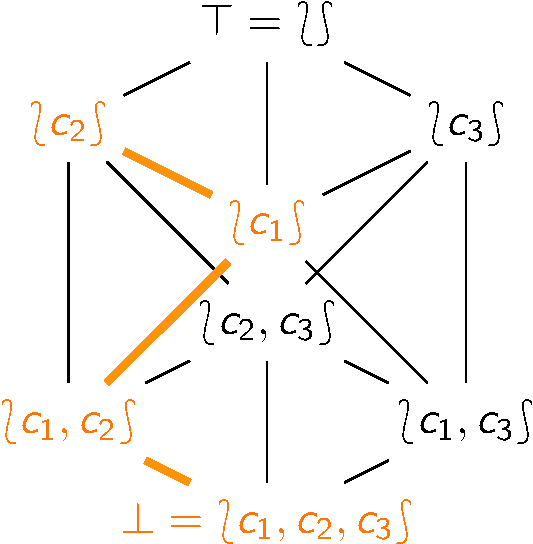
\includegraphics[width=2.3cm]{img/search-space.pdf} }; 

\node[anchor=west,font=\small] at (5.7,-1.3) {$\mathit{PVS}\langle P \rangle $};
\node[anchor=west,font=\normalsize] at (5.7,-3.6) {$\langle \finmsets(P), \mcup, \smytheq{P}, \lbag \rbag \rangle$};

\node[constraint,label=west:$\lbag \mathrm{c}_1 \rbag$] (p1) at (7, -2)                   {$\mathrm{c}_1$};
\node[constraint,label=east:$\lbag \mathrm{c}_2 \rbag$] (p2) at ($ (p1) + (-0.8, -0.8) $) {$\mathrm{c}_2$};  
\node[constraint,label=north:$\lbag \mathrm{c}_3 \rbag$] (p3) at ($ (p1) + ( 0.8, -0.8) $) {$\mathrm{c}_3$};  
%  
\path[every node/.style={font=\sffamily\tiny}]
  (p2) edge (p1)
  (p3) edge (p1)
  ;

\end{tikzpicture}

\begin{lstlisting}
solve constraintPrefs1;
\end{lstlisting}
    \end{column}
    \begin{column}{.45\textwidth}
    \centering \hSecond{Weighted}
    
    \vspace*{2ex}
    
    \begin{tikzpicture}[auto,->,
                    >=stealth',shorten >=1pt,thick,
                    node distance=.7cm,inner sep=2pt,
                    constraint/.style={circle,fill=black!15,draw,font=\sffamily\small},
                    bg/.style={shape=rectangle, rounded corners,
    draw, align=center,
    top color=white, bottom color=issegrey!15},
                    pvs/.style={shape=rectangle, rounded corners,
    draw=isseorange!50,fill=white, align=center}]

\node[pvs,draw=CornflowerBlue,text width=3.5cm,anchor=north west, text height=2.8cm] at (0.5,-1) {};
 \node[anchor=west,font=\small] at (0.5,-1.3) {$\mathit{Weighted}(P)$};
  \node[anchor=west,font=\normalsize] at (0.5,-3.6) {$\langle \mathbb{N}, +, \geq, 0 \rangle$};
  
\node[constraint,label=west:2] (w1) at (2, -2)                   {$\mathrm{c}_1$};
\node[constraint,label=west:1] (w2) at ($ (w1) + (-0.8, -0.8) $) {$\mathrm{c}_2$};  
\node[constraint,label=west:1] (w3) at ($ (w1) + ( 0.8, -0.8) $) {$\mathrm{c}_3$};  
\node at (3.6, -2.4) {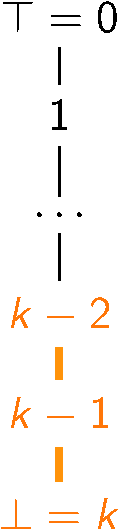
\includegraphics[width=.55cm]{img/search-space-weighted.pdf} }; 

%  
\path[every node/.style={font=\sffamily\tiny}]
  (w2) edge (w1)
  (w3) edge (w1)
  ;
 

\end{tikzpicture}
\begin{lstlisting}
solve ToWeighted(constraintPrefs1);
\end{lstlisting}
    \end{column}
  \end{columns}  
  
\begin{parchment}[Evaluationsfrage]
Ist es wesentlich teurer nach Smyth zu optimieren, anstatt ein gewichtetes Problem zu verwenden?

\end{parchment}
\end{frame}

\begin{frame}{Vergleich Weighted vs Constraint Preferences}
\vspace*{4ex}

\begin{table}
\centering
{
\scriptsize
\begin{tabular*}{\textwidth}{@{\extracolsep{\fill} }ld{1.1}d{1.1}d{1.1}d{1.1}d{1.1}}
\toprule
\multicolumn{1}{c}{Solver} & \multicolumn{1}{c}{Time Smyth} 
          & \multicolumn{1}{c}{Time Weighted} 
          & \multicolumn{1}{c}{Time Toulbar2}
          & \multicolumn{1}{c}{Obj. Weights} & \multicolumn{1}{c}{Obj. Smyth}   \\
\midrule
\multicolumn{2}{l}{MSPSP (6 instances)  }   \\
\midrule
   Gecode & 12.74 & \textbf{0}.\textbf{34} & - & 2.67 & 5.50 \\
   Native Gecode & 7.82 & \textbf{0}.\textbf{26} & - & 2.80 & 5.80 \\
   JaCoP & 4.18 & \textbf{0}.\textbf{45} & - & 2.00 & 6.00 \\
\midrule
\multicolumn{2}{l}{On-Call Rostering (5 instances)  }   \\
\midrule
   Gecode & 220.46 & \textbf{133}.\textbf{32} & (14.52) & 3.20 & 7.20 \\
   Native Gecode & 192.50 & \textbf{133}.\textbf{32} & (14.52) & 3.20 & 25.20 \\
   JaCoP & 194.06 & \textbf{135}.\textbf{28} & (14.52) & 3.20 & 26.80 \\
\midrule
\multicolumn{2}{l}{Photo Placement (3 instances)  }   \\
\midrule
   Gecode & 6.69 & \textbf{1}.\textbf{03} & (0.68) & 13.00 & 13.00 \\
   Native Gecode & \textbf{9}.\textbf{96} & 22.22 & (0.80) & 13.33 & 13.33 \\
   JaCoP & 15.73 & \textbf{3}.\textbf{18} & (0.80) & 13.33 & 13.33 \\
\midrule
\multicolumn{2}{l}{Soft N-Queens (3 instances)  }   \\
\midrule
   Gecode & \textbf{3}.\textbf{45} & 210.02 & (0.30) & 1.67 & 2.00 \\
   Native Gecode & \textbf{3}.\textbf{49} & 210.02 & (0.30) & 1.67 & 1.33 \\
   JaCoP & \textbf{3}.\textbf{94} & 57.22 & (0.30) & 0.33 & 1.00 \\
\midrule
\multicolumn{2}{l}{Talent Scheduling (6 instances)  }   \\
\midrule
   Gecode & \textbf{7}.\textbf{78} & 158.94 & - & 12.50 & 14.25 \\
   Native Gecode & \textbf{13}.\textbf{50} & 141.09 & - & 12.33 & 14.67 \\
   JaCoP & \textbf{15}.\textbf{63} & 120.42 & - & 12.33 & 14.17 \\
\bottomrule
\end{tabular*}

}
\end{table}
\end{frame}
\tikzstyle{highlight}=[isseorange,ultra thick]
\tikzstyle{highlight2}=[CornflowerBlue,ultra thick]

\begin{frame}[fragile]{Nicht-Dominiert versus Strikte Verbesserung}
\vspace*{6ex}

\begin{columns}[onlytextwidth]
    \begin{column}{.45\textwidth}
    \centering \hSecond{Nicht-Dominiert}
    
    \vspace*{2ex}
    
\begin{tikzpicture}[scale=0.5,transform shape,auto]

% single PVS
\node [highlight2] (bot) at (0,0) {$\bot = \{c_1, c_2, c_3 \}$};
\node [highlight2] (c1c2) at (-2,1) {$\{c_1, c_2\}$};
\node[highlight2] (c2c3) at (0,2) {$\{c_2, c_3\}$};
\node (c1c3) at (2,1) {$\{c_1, c_3\}$};

\node (c1) at (0,3) {$\{c_1\}$};
\node [highlight2] (c2) at (-2,4) {$\{c_2\}$};
\node [highlight2](c3) at (2,4) {$\{c_3\}$};
%\node (a) at (-1,0.5) {$a$};
%\node (b) at (-1,1.5) {$b$};
%\node (c) at (1,1) {$c$};
\node (top) at (0,5) {$\top = \emptyset$};


\path[-]
(bot) edge[highlight2](c1c2)
      edge (c2c3)
      edge (c1c3)
(c1c2) edge[highlight2] (c2c3)
(c1c3) edge (c2c3)
(c1c3) edge (c1)
(c1c3) edge (c3)
(c2c3) edge[highlight2] (c2)
(c2c3) edge[highlight2] (c3)
(c1c2) edge (c1)
(c1c2) edge (c2)
(c1) edge (c2)
(c1) edge (c3)
(c2) edge (top)
(c1) edge (top)
(c3) edge (top)
      ;

\end{tikzpicture}

\begin{lstlisting}
solve 
search pvs_BAB_NonDom();  
\end{lstlisting}
    \end{column}
    \begin{column}{.45\textwidth}
    \centering \hFirst{Strikte Verbesserung}
    
    \vspace*{2ex}
    
\begin{tikzpicture}[scale=0.5,transform shape,auto]

% single PVS
\node (bot) at (0,0) {\alert{$\bot = \{c_1, c_2, c_3 \}$}};
\node (c1c2) at (-2,1) {\alert{$\{c_1, c_2\}$}};
\node (c2c3) at (0,2) {\alert{$\{c_2, c_3\}$}};
\node (c1c3) at (2,1) {$\{c_1, c_3\}$};

\node (c1) at (0,3) {$\{c_1\}$};
\node (c2) at (-2,4) {\alert{$\{c_2\}$}};
\node (c3) at (2,4) {$\{c_3\}$};
%\node (a) at (-1,0.5) {$a$};
%\node (b) at (-1,1.5) {$b$};
%\node (c) at (1,1) {$c$};
\node (top) at (0,5) {$\top = \emptyset$};


\path[-]
(bot) edge[highlight] (c1c2)
      edge (c2c3)
      edge (c1c3)
(c1c2) edge[highlight]  (c2c3)
(c1c3) edge (c2c3)
(c1c3) edge (c1)
(c1c3) edge (c3)
(c2c3) edge[highlight]  (c2)
(c2c3) edge (c3)
(c1c2) edge (c1)
(c1c2) edge (c2)
(c1) edge (c2)
(c1) edge (c3)
(c2) edge (top)
(c1) edge (top)
(c3) edge (top)
      ;

\end{tikzpicture}

\begin{lstlisting}
solve 
search pvs_BAB();  
\end{lstlisting}
    \end{column}
  \end{columns}  
  
\begin{parchment}[Evaluationsfrage]
Wieviel Overhead erzeugt das Suchen aller (unvergleichbar) optimalen Lösungen gegenüber dem Suchein \emph{einer} optimalen Lösung?
\end{parchment}
\end{frame}


\begin{frame}[fragile]{Nicht-Dominiert versus Strikte Verbesserung}
\begin{columns}[onlytextwidth]
    \begin{column}{.45\textwidth}
    \centering \hSecond{Nicht-Dominiert}
    
    \vspace*{2ex}
    
\begin{tikzpicture}[scale=0.5,transform shape,auto]

% single PVS
\node [highlight2] (bot) at (0,0) {$\bot = \{c_1, c_2, c_3 \}$};
\node [highlight2] (c1c2) at (-2,1) {$\{c_1, c_2\}$};
\node[highlight2] (c2c3) at (0,2) {$\{c_2, c_3\}$};
\node (c1c3) at (2,1) {$\{c_1, c_3\}$};

\node (c1) at (0,3) {$\{c_1\}$};
\node [highlight2] (c2) at (-2,4) {$\{c_2\}$};
\node [highlight2](c3) at (2,4) {$\{c_3\}$};
%\node (a) at (-1,0.5) {$a$};
%\node (b) at (-1,1.5) {$b$};
%\node (c) at (1,1) {$c$};
\node (top) at (0,5) {$\top = \emptyset$};


\path[-]
(bot) edge[highlight2](c1c2)
      edge (c2c3)
      edge (c1c3)
(c1c2) edge[highlight2] (c2c3)
(c1c3) edge (c2c3)
(c1c3) edge (c1)
(c1c3) edge (c3)
(c2c3) edge[highlight2] (c2)
(c2c3) edge[highlight2] (c3)
(c1c2) edge (c1)
(c1c2) edge (c2)
(c1) edge (c2)
(c1) edge (c3)
(c2) edge (top)
(c1) edge (top)
(c3) edge (top)
      ;

\end{tikzpicture}

    \end{column}
    \begin{column}{.45\textwidth}
    \centering \hFirst{Strikte Verbesserung}
    
    \vspace*{2ex}
    
\begin{tikzpicture}[scale=0.5,transform shape,auto]

% single PVS
\node (bot) at (0,0) {\alert{$\bot = \{c_1, c_2, c_3 \}$}};
\node (c1c2) at (-2,1) {\alert{$\{c_1, c_2\}$}};
\node (c2c3) at (0,2) {\alert{$\{c_2, c_3\}$}};
\node (c1c3) at (2,1) {$\{c_1, c_3\}$};

\node (c1) at (0,3) {$\{c_1\}$};
\node (c2) at (-2,4) {\alert{$\{c_2\}$}};
\node (c3) at (2,4) {$\{c_3\}$};
%\node (a) at (-1,0.5) {$a$};
%\node (b) at (-1,1.5) {$b$};
%\node (c) at (1,1) {$c$};
\node (top) at (0,5) {$\top = \emptyset$};


\path[-]
(bot) edge[highlight] (c1c2)
      edge (c2c3)
      edge (c1c3)
(c1c2) edge[highlight]  (c2c3)
(c1c3) edge (c2c3)
(c1c3) edge (c1)
(c1c3) edge (c3)
(c2c3) edge[highlight]  (c2)
(c2c3) edge (c3)
(c1c2) edge (c1)
(c1c2) edge (c2)
(c1) edge (c2)
(c1) edge (c3)
(c2) edge (top)
(c1) edge (top)
(c3) edge (top)
      ;

\end{tikzpicture}

    \end{column}
  \end{columns}  
\begin{table}
\centering
{
\scriptsize

\label{tab:compDomNonDom}


\begin{tabular*}{\textwidth}{@{\extracolsep{\fill} }ld{1.1}d{1.1}d{1.1}d{1.1}}
\toprule
\multicolumn{1}{c}{Problem} & \multicolumn{1}{c}{Time Non-Dominated BaB} 
          & \multicolumn{1}{c}{Time Strict BaB} 
          & \multicolumn{1}{c}{Absolute Overhead}
          & \multicolumn{1}{c}{Relative Overhead}   \\
\midrule
   MSPSP & \textbf{7}.\textbf{31} & 8.89 & -1.58 & 1.50 \\
   On-Call Rostering & 329.44 & \textbf{199}.\textbf{21} & 130.23 & 1.82 \\
   Photo Placement & 55.09 & \textbf{7}.\textbf{51} & 47.58 & 9.72 \\
   Soft N-Queens & \textbf{2}.\textbf{24} & 3.65 & -1.41 & 1.91 \\
   Talent Scheduling & 33.44 & \textbf{12}.\textbf{24} & 21.21 & 2.30 \\
\midrule
\emph{Overall} & 102.00 & \textbf{57}.\textbf{20} & 44.80 & 2.97 \\
\bottomrule
\end{tabular*}
}
\end{table}

\end{frame}

\begin{frame}[fragile]{Vergleich MIF vs. Standard}
\vspace*{2ex}

\begin{lstlisting}
type WeightedCsp = PVSType<bool, int> = 
  params {[..]  } in  
  instantiates with "soft_constraints/mbr_types/weighted_type.mzn" { [...] }
 offers {
    heuristics -> getSearchHeuristicWeighted;
 };
 \end{lstlisting}

\begin{columns}[onlytextwidth]
    \begin{column}{.45\textwidth}
    \centering \hFirst{Most-Important First}

    \vspace*{1ex}

\begin{lstlisting}
solve 
:: pvsSearchHeuristic
search pvs_BAB();
\end{lstlisting}
    \end{column}
    \begin{column}{.45\textwidth}
    \centering \hSecond{Standard-Suche}

    \vspace*{1ex}
    \begin{lstlisting}
solve 
search pvs_BAB();
\end{lstlisting}
    \end{column}
\end{columns}
\begin{parchment}[Evaluationsfrage]
Kann die generische MIF-Suchheuristik die Suche nach Optima beschleunigen?
\end{parchment}
\end{frame}

\begin{frame}{Vergleich MIF vs. Standard I}
\begin{table}
\centering
{
\scriptsize

\label{tab:compDiffsMif}


\subcaption*{Gruppiert nach Solvern.}
\begin{tabular*}{\textwidth}{@{\extracolsep{\fill} }ld{1.1}d{1.1}d{1.1}d{1.1}d{1.1}d{1.1}d{1.1}}
\toprule
 &  \multicolumn{1}{c}{Choco} & \multicolumn{1}{c}{G12} & \multicolumn{1}{c}{Gecode} & \multicolumn{1}{c}{JaCoP} & \multicolumn{1}{c}{Toulbar2} & \multicolumn{1}{c}{OR-Tools} \\
\midrule
Instances &  28 & 28 & 28 & 28 & 28 & 28 \\
Runtime difference &  -73.14 & -17.57 & -18.42 & 16.15 & 36.63 & 19.05 \\
Ratio MIF wins &  0.64 & 0.32 & 0.29 & 0.46 & 0.57 & 0.32 \\
\bottomrule
\end{tabular*}

\bigskip
\subcaption*{Gruppiert nach Problemen.}

\begin{tabular*}{\textwidth}{@{\extracolsep{\fill} }ld{1.1}d{1.1}d{1.1}d{1.1}d{1.1}d{1.1}}
\toprule
 &  \multicolumn{1}{c}{MSPSP} & \multicolumn{1}{c}{On-Call Rostering} & \multicolumn{1}{c}{Photo Placement} & \multicolumn{1}{c}{Soft N-Queens} & \multicolumn{1}{c}{Talent Scheduling} \\
\midrule
Instances &  48 & 42 & 18 & 18 & 42 \\
Runtime difference &  -0.80 & -31.04 & 141.17 & -79.51 & -19.34 \\
Ratio MIF wins &  0.42 & 0.55 & 0.06 & 0.56 & 0.45 \\
\bottomrule
\end{tabular*}
}
\end{table}
\end{frame}

\begin{frame}{Vergleich MIF vs. Standard II}
\begin{figure}
	\centering
	\begin{subfigure}[b]{.48\textwidth}
		\centering
		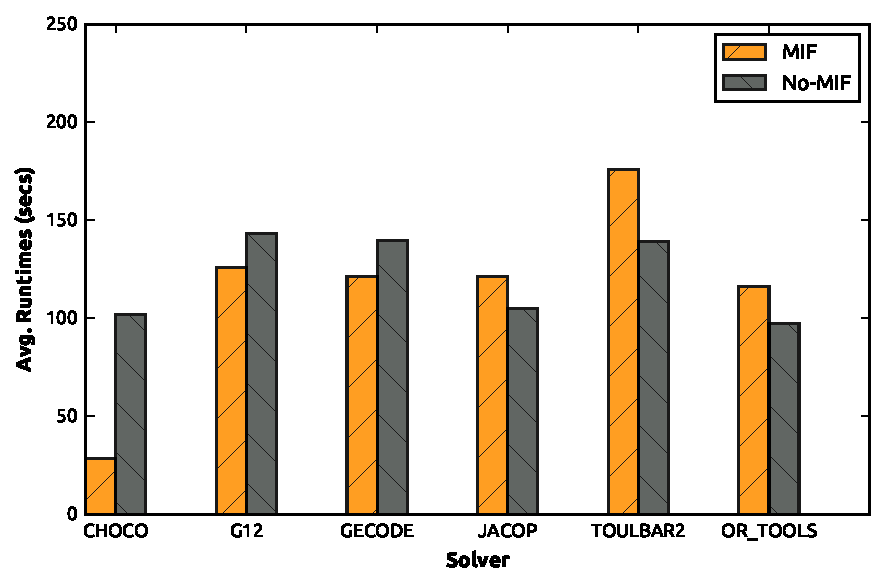
\includegraphics[width=\textwidth]{img/runtime-mif-solver.pdf} %TODO: check: how were the 8 points sampled? Not uniformly...
         \caption{Runtimes grouped by solver for MIF on/off.}
		\label{fig:runtimesMIFSolvers}
	\end{subfigure}%
	~ \quad%add desired spacing between images, e. g. ~, \quad, \qquad, \hfill etc.
	%(or a blank line to force the subfigure onto a new line)
	\begin{subfigure}[b]{.48\textwidth}
		\centering
		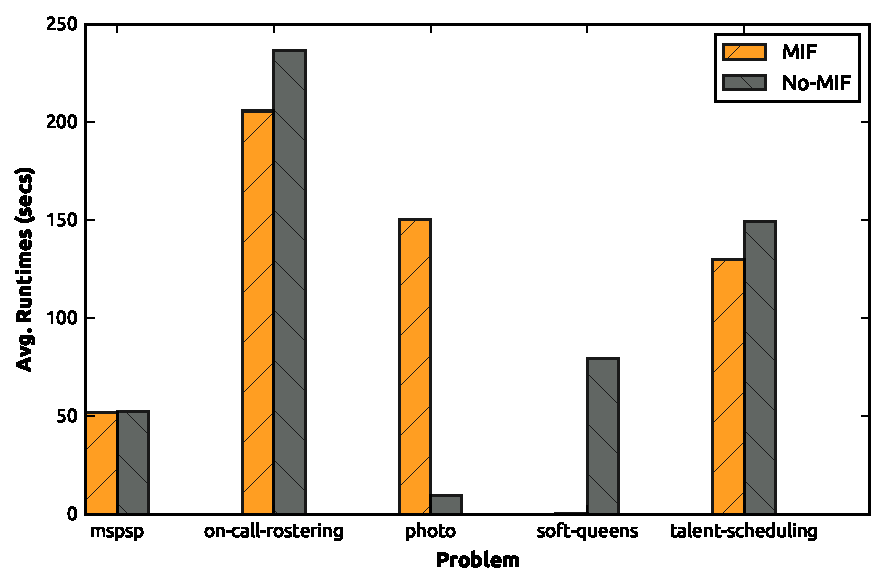
\includegraphics[width=\textwidth]{img/runtime-mif-problem.pdf}
		\caption{Runtimes grouped by problem for MIF on/off.}
		\label{fig:runtimesMIFProblems}
	\end{subfigure}

	\label{fig:runtimesMIF}
\end{figure}
\end{frame}

\begin{frame}{Zusammenfassung}

\begin{enumerate}
\item Weitgehende algebraische Konzepte zur Modellierung von Präferenzstrukturen in der Literatur
\item Free PVS, Constraint Preferences, PVS-Produkte für Hierarchien $\checkmark$ \pause 
\vspace*{1ex}
\item Es gibt genau einen dedizierten Soft-Constraint-Solver, \texttt{toulbar2} für weighted CSP; wir können abstraktere Typen behandeln
\vspace*{1ex} \pause 
\item Modellierungssprache für Präferenzen weiterentwickelt $\checkmark$
\begin{itemize}
\item[-] Graphische Schnittstelle (benutzer-orientiert) $\checkmark$
\item[-] Unsere gängigen Fallstudien lassen sich abbilden $\checkmark$
\item[-] Erweiterbarkeit gegeben $\checkmark$
\end{itemize}
\vspace*{1ex}
\pause 
\item Ausführliche Evaluierung auf \alert{Benchmark}-Problemen demonstriert Vorteile durch Solver-Unabhängigkeit: Für z.B. Scheduling-Probleme sind Reduktionen schneller als dedizierte Soft-Constraint-Solver
\item Optimierung nach abstrakten Ordnungen problemlos möglich; Übergang zwischen PVS-Modellen leicht
\end{enumerate}
\end{frame}






\begin{frame}[allowframebreaks]
        \frametitle{References}
        \bibliographystyle{apalike}
        \bibliography{../common}
\end{frame}


\end{document}

